% Plantilla para un Trabajo Fin de Grado de la Universidad de Granada,
% adaptada para el Doble Grado en Ingeniería Informática y Matemáticas.
%
%  Autor: Miguel Ángel Cantarero.
%  Licencia: GNU GPLv2.
%
% Esta plantilla es una adaptación al castellano de la plantilla
% classicthesis de André Miede, que puede obtenerse en:
%  https://ctan.org/tex-archive/macros/latex/contrib/classicthesis?lang=en
% La plantilla original se licencia en GNU GPLv2.
%
% Esta plantilla usa símbolos de la Universidad de Granada sujetos a la normativa
% de identidad visual corporativa, que puede encontrarse en:
% http://secretariageneral.ugr.es/pages/ivc/normativa
%
% La compilación se realiza con las siguientes instrucciones:
%   pdflatex --shell-escape main.tex
%   bibtex main
%   pdflatex --shell-escape main.tex

% Opciones del tipo de documento
\documentclass[oneside,openright,titlepage,numbers=noenddot,openany,headinclude,footinclude=true,
cleardoublepage=empty,abstractoff,BCOR=5mm,paper=a4,fontsize=12pt,main=spanish]{scrreprt}

% Paquetes de latex que se cargan al inicio. Cubren la entrada de
% texto, gráficos, código fuente y símbolos.
\usepackage[table]{xcolor}
\usepackage[hyphens]{url}
\usepackage[utf8]{inputenc}
\usepackage[T1]{fontenc}
\usepackage{fixltx2e}
\usepackage{subfig}
\usepackage{graphicx} % Inclusión de imágenes.
\usepackage{grffile}  % Distintos formatos para imágenes.
\usepackage{longtable} % Tablas multipágina.
\usepackage{wrapfig} % Coloca texto alrededor de una figura.
\usepackage{rotating}
\usepackage[normalem]{ulem}
\usepackage{amsmath}
\usepackage{textcomp}
\usepackage{amssymb}
\usepackage{capt-of}
\usepackage[colorlinks=true]{hyperref}
\usepackage{tikz} % Diagramas conmutativos.
\usepackage{minted} % Código fuente.
\usepackage[T1]{fontenc}
\usepackage{natbib}
\usepackage{tikz}
\usepackage[spanish,es-tabla]{babel}

% Plantilla classicthesis
\usepackage[beramono,eulerchapternumbers,linedheaders,parts,a5paper,dottedtoc,
manychapters,pdfspacing]{classicthesis}

% Geometría y espaciado de párrafos.
\setcounter{secnumdepth}{0}
\usepackage{enumitem}
\setitemize{noitemsep,topsep=0pt,parsep=0pt,partopsep=0pt}
\setlist[enumerate]{topsep=0pt,itemsep=-1ex,partopsep=1ex,parsep=1ex}
\usepackage[top=1in, bottom=1.5in, left=1in, right=1in]{geometry}
\setlength\itemsep{0em}
\setlength{\parindent}{0pt}
\usepackage{parskip}
\usepackage{textcomp}
% Profundidad de la tabla de contenidos.
\setcounter{secnumdepth}{3}

% Usa el paquete minted para mostrar trozos de código.
% Pueden seleccionarse el lenguaje apropiado y el estilo del código.
\usepackage{minted}
\usemintedstyle{colorful}
\setminted{fontsize=\small}
\setminted[python]{linenos=false,fontsize=\small}
\renewcommand{\theFancyVerbLine}{\sffamily\textcolor[rgb]{0.5,0.5,1.0}{\oldstylenums{\arabic{FancyVerbLine}}}}

% Archivos de configuración.
%------------------------
% Bibliotecas para matemáticas de latex
%------------------------
\usepackage{amsthm}
\usepackage{amsmath}
\usepackage[ruled, spanish, onelanguage, linesnumbered]{algorithm2e}
\usepackage{tikz}
\usepackage{tikz-cd}
\usetikzlibrary{shapes,fit}
\usepackage{bussproofs}
\EnableBpAbbreviations{}
\usepackage{mathtools}
\usepackage{scalerel}
\usepackage{stmaryrd}

%------------------------
% Estilos para los teoremas
%------------------------
\theoremstyle{plain}
\newtheorem{theorem}{Teorema}
\newtheorem{proposition}{Proposición}
\newtheorem{lemma}{Lema}
\newtheorem{corollary}{Corolario}
\theoremstyle{definition}
\newtheorem{definition}{Definición}
\newtheorem{proofs}{Demostración}
\theoremstyle{remark}
\newtheorem{remark}{Comentario}
\newtheorem{exampleth}{Ejemplo}

\begingroup\makeatletter\@for\theoremstyle:=definition,remark,plain\do{\expandafter\g@addto@macro\csname th@\theoremstyle\endcsname{\addtolength\thm@preskip\parskip}}\endgroup

%------------------------
% Macros
% ------------------------

% Aquí pueden añadirse abreviaturas para comandos de latex
% frequentemente usados.
\newcommand*\diff{\mathop{}\!\mathrm{d}}
% Fracción grande: \ddfrac{}{}
\newcommand\ddfrac[2]{\frac{\displaystyle #1}{\displaystyle #2}}
% Valor absoluto: \abs{}
\providecommand{\abs}[1]{\lvert#1\rvert}   
% Licencia
\usepackage[
    type={CC},
    modifier={by-sa},
    version={4.0},
]{doclicense}

\newcommand{\R}{\mathbb{R}}
\newcommand{\M}{\mathcal{M}}
\newcommand{\I}{\mathcal{I}}

\renewcommand\L{\mathcal{L}}
\newcommand{\G}{\mathcal{G}}
\newcommand\m[1]{\mathcal{#1}}
  % En macros.tex se almacenan las opciones y comandos para escribir matemáticas.
\graphicspath{ {./images/} }
% ****************************************************************************************************
% classicthesis-config.tex 
% formerly known as loadpackages.sty, classicthesis-ldpkg.sty, and classicthesis-preamble.sty 
% Use it at the beginning of your ClassicThesis.tex, or as a LaTeX Preamble 
% in your ClassicThesis.{tex,lyx} with % ****************************************************************************************************
% classicthesis-config.tex 
% formerly known as loadpackages.sty, classicthesis-ldpkg.sty, and classicthesis-preamble.sty 
% Use it at the beginning of your ClassicThesis.tex, or as a LaTeX Preamble 
% in your ClassicThesis.{tex,lyx} with % ****************************************************************************************************
% classicthesis-config.tex 
% formerly known as loadpackages.sty, classicthesis-ldpkg.sty, and classicthesis-preamble.sty 
% Use it at the beginning of your ClassicThesis.tex, or as a LaTeX Preamble 
% in your ClassicThesis.{tex,lyx} with \input{classicthesis-config}
% ****************************************************************************************************  
% If you like the classicthesis, then I would appreciate a postcard. 
% My address can be found in the file ClassicThesis.pdf. A collection 
% of the postcards I received so far is available online at 
% http://postcards.miede.de
% ****************************************************************************************************


% ****************************************************************************************************
% 0. Set the encoding of your files. UTF-8 is the only sensible encoding nowadays. If you can't read
% äöüßáéçèê∂åëæƒÏ€ then change the encoding setting in your editor, not the line below. If your editor
% does not support utf8 use another editor!
% ****************************************************************************************************
\PassOptionsToPackage{utf8x}{inputenc}
	\usepackage{inputenc}

% ****************************************************************************************************
% 1. Configure classicthesis for your needs here, e.g., remove "drafting" below 
% in order to deactivate the time-stamp on the pages
% ****************************************************************************************************
\PassOptionsToPackage{eulerchapternumbers,listings,drafting,%
		pdfspacing,%floatperchapter,%linedheaders,%
                subfig,beramono,eulermath,parts,dottedtoc}{classicthesis}                                        
% ********************************************************************
% Available options for classicthesis.sty 
% (see ClassicThesis.pdf for more information):
% drafting
% parts nochapters linedheaders
% eulerchapternumbers beramono eulermath pdfspacing minionprospacing
% tocaligned dottedtoc manychapters
% listings floatperchapter subfig
% ********************************************************************

% ****************************************************************************************************
% 2. Personal data and user ad-hoc commands
% ****************************************************************************************************
\newcommand{\myTitle}{TFG-FCA-MiguelCantarero\xspace}
\newcommand{\mySubtitle}{Estudio Experimental Algoritmos FCA\xspace}
\newcommand{\myDegree}{Doble Grado en Ingeniería Informática y Matemáticas\xspace}
\newcommand{\myName}{Miguel Cantarero\xspace}
\newcommand{\myProf}{Nicolás Marín\xspace}
\newcommand{\myOtherProf}{Daniel Sánchez\xspace}
\newcommand{\mySupervisor}{Put name here\xspace}
\newcommand{\myFaculty}{Universidad de Granada\xspace}
\newcommand{\myDepartment}{Put data here\xspace}
\newcommand{\myUni}{Put data here\xspace}
\newcommand{\myLocation}{Saarbrücken\xspace}
\newcommand{\myTime}{September 2015\xspace}
%\newcommand{\myVersion}{version 4.2\xspace}

% ********************************************************************
% Setup, finetuning, and useful commands
% ********************************************************************
\newcounter{dummy} % necessary for correct hyperlinks (to index, bib, etc.)
\newlength{\abcd} % for ab..z string length calculation
\providecommand{\mLyX}{L\kern-.1667em\lower.25em\hbox{Y}\kern-.125emX\@}
\newcommand{\ie}{i.\,e.}
\newcommand{\Ie}{I.\,e.}
\newcommand{\eg}{e.\,g.}
\newcommand{\Eg}{E.\,g.} 
% ****************************************************************************************************


% ****************************************************************************************************
% 3. Loading some handy packages
% ****************************************************************************************************
% ******************************************************************** 
% Packages with options that might require adjustments
% ******************************************************************** 
%\PassOptionsToPackage{ngerman,american}{babel}   % change this to your language(s)
% Spanish languages need extra options in order to work with this template
% \PassOptionsToPackage{es-lcroman,spanish}{babel}
\usepackage[spanish,es-tabla]{babel}



%\usepackage{csquotes}
% \PassOptionsToPackage{%
%     %backend=biber, %instead of bibtex
% 	backend=bibtex8,bibencoding=ascii,%
% 	language=auto,%
% 	style=alpha,%
%     %style=authoryear-comp, % Author 1999, 2010
%     %bibstyle=authoryear,dashed=false, % dashed: substitute rep. author with ---
%     sorting=nyt, % name, year, title
%     maxbibnames=10, % default: 3, et al.
%     %backref=true,%
%     natbib=true % natbib compatibility mode (\citep and \citet still work)
% }{biblatex}
%     \usepackage{biblatex}

% \PassOptionsToPackage{fleqn}{amsmath}       % math environments and more by the AMS 
%     \usepackage{amsmath}

% ******************************************************************** 
% General useful packages
% ******************************************************************** 
\PassOptionsToPackage{T1}{fontenc} % T2A for cyrillics
    \usepackage{fontenc}     
\usepackage{textcomp} % fix warning with missing font shapes
\usepackage{scrhack} % fix warnings when using KOMA with listings package          
\usepackage{xspace} % to get the spacing after macros right  
\usepackage{mparhack} % get marginpar right
\usepackage{fixltx2e} % fixes some LaTeX stuff --> since 2015 in the LaTeX kernel (see below)
%\usepackage[latest]{latexrelease} % will be used once available in more distributions (ISSUE #107)
\PassOptionsToPackage{printonlyused,smaller}{acronym} 
    \usepackage{acronym} % nice macros for handling all acronyms in the thesis
    %\renewcommand{\bflabel}[1]{{#1}\hfill} % fix the list of acronyms --> no longer working
    %\renewcommand*{\acsfont}[1]{\textsc{#1}} 
    \renewcommand*{\aclabelfont}[1]{\acsfont{#1}}
% ****************************************************************************************************


% ****************************************************************************************************
% 4. Setup floats: tables, (sub)figures, and captions
% ****************************************************************************************************
\usepackage{tabularx} % better tables
    \setlength{\extrarowheight}{3pt} % increase table row height
\newcommand{\tableheadline}[1]{\multicolumn{1}{c}{\spacedlowsmallcaps{#1}}}
\newcommand{\myfloatalign}{\centering} % to be used with each float for alignment
\usepackage{caption}
% Thanks to cgnieder and Claus Lahiri
% http://tex.stackexchange.com/questions/69349/spacedlowsmallcaps-in-caption-label
% [REMOVED DUE TO OTHER PROBLEMS, SEE ISSUE #82]    
%\DeclareCaptionLabelFormat{smallcaps}{\bothIfFirst{#1}{~}\MakeTextLowercase{\textsc{#2}}}
%\captionsetup{font=small,labelformat=smallcaps} % format=hang,
\captionsetup{font=small} % format=hang,
\usepackage{subfig}  
% ****************************************************************************************************


% ****************************************************************************************************
% 5. Setup code listings
% ****************************************************************************************************
% \usepackage{listings} 
% %\lstset{emph={trueIndex,root},emphstyle=\color{BlueViolet}}%\underbar} % for special keywords
% \lstset{language={Haskell},morekeywords={PassOptionsToPackage,selectlanguage},keywordstyle=\color{RoyalBlue},basicstyle=\small\ttfamily,commentstyle=\color{Green}\ttfamily,stringstyle=\rmfamily,numbers=none,numberstyle=\scriptsize,stepnumber=5,numbersep=8pt,showstringspaces=false,breaklines=true,belowcaptionskip=.75\baselineskip} 
% ****************************************************************************************************             


% ****************************************************************************************************
% 6. PDFLaTeX, hyperreferences and citation backreferences
% ****************************************************************************************************
% ********************************************************************
% Using PDFLaTeX
% ********************************************************************
\PassOptionsToPackage{pdftex,hyperfootnotes=false,pdfpagelabels}{hyperref}
    \usepackage{hyperref}  % backref linktocpage pagebackref
\pdfcompresslevel=9
\pdfadjustspacing=1 
\PassOptionsToPackage{pdftex}{graphicx}
    \usepackage{graphicx} 
 

% ********************************************************************
% Hyperreferences
% ********************************************************************
\hypersetup{%
    %draft, % = no hyperlinking at all (useful in b/w printouts)
    colorlinks=true, linktocpage=true, pdfstartpage=3, pdfstartview=FitV,%
    % uncomment the following line if you want to have black links (e.g., for printing)
    %colorlinks=false, linktocpage=false, pdfstartpage=3, pdfstartview=FitV, pdfborder={0 0 0},%
    breaklinks=true, pdfpagemode=UseNone, pageanchor=true, pdfpagemode=UseOutlines,%
    plainpages=false, bookmarksnumbered, bookmarksopen=true, bookmarksopenlevel=1,%
    hypertexnames=true, pdfhighlight=/O,%nesting=true,%frenchlinks,%
    urlcolor=webbrown, linkcolor=RoyalBlue, citecolor=webgreen, %pagecolor=RoyalBlue,%
    %urlcolor=Black, linkcolor=Black, citecolor=Black, %pagecolor=Black,%
    pdftitle={\myTitle},%
    pdfauthor={\textcopyright\ \myName, \myUni, \myFaculty},%
    pdfsubject={},%
    pdfkeywords={},%
    pdfcreator={pdfLaTeX},%
    pdfproducer={LaTeX with hyperref and classicthesis}%
}   

% ********************************************************************
% Setup autoreferences
% ********************************************************************
% There are some issues regarding autorefnames
% http://www.ureader.de/msg/136221647.aspx
% http://www.tex.ac.uk/cgi-bin/texfaq2html?label=latexwords
% you have to redefine the makros for the 
% language you use, e.g., american, ngerman
% (as chosen when loading babel/AtBeginDocument)
% ********************************************************************
\makeatletter
\@ifpackageloaded{babel}%
    {%
       \addto\extrasamerican{%
			\renewcommand*{\figureautorefname}{Figure}%
			\renewcommand*{\tableautorefname}{Table}%
			\renewcommand*{\partautorefname}{Part}%
			\renewcommand*{\chapterautorefname}{Chapter}%
			\renewcommand*{\sectionautorefname}{Section}%
			\renewcommand*{\subsectionautorefname}{Section}%
			\renewcommand*{\subsubsectionautorefname}{Section}%     
                }%
       \addto\extrasngerman{% 
			\renewcommand*{\paragraphautorefname}{Absatz}%
			\renewcommand*{\subparagraphautorefname}{Unterabsatz}%
			\renewcommand*{\footnoteautorefname}{Fu\"snote}%
			\renewcommand*{\FancyVerbLineautorefname}{Zeile}%
			\renewcommand*{\theoremautorefname}{Theorem}%
			\renewcommand*{\appendixautorefname}{Anhang}%
			\renewcommand*{\equationautorefname}{Gleichung}%        
			\renewcommand*{\itemautorefname}{Punkt}%
                }%  
            % Fix to getting autorefs for subfigures right (thanks to Belinda Vogt for changing the definition)
            \providecommand{\subfigureautorefname}{\figureautorefname}%             
    }{\relax}
\makeatother


% ****************************************************************************************************
% 7. Last calls before the bar closes
% ****************************************************************************************************
% ********************************************************************
% Development Stuff
% ********************************************************************
\listfiles
%\PassOptionsToPackage{l2tabu,orthodox,abort}{nag}
%   \usepackage{nag}
%\PassOptionsToPackage{warning, all}{onlyamsmath}
%   \usepackage{onlyamsmath}

% ********************************************************************
% Last, but not least...
% ********************************************************************
\usepackage{classicthesis} 
% ****************************************************************************************************


% ****************************************************************************************************
% 8. Further adjustments (experimental)
% ****************************************************************************************************
% ********************************************************************
% Changing the text area
% ********************************************************************
%\linespread{1.05} % a bit more for Palatino
%\areaset[current]{312pt}{761pt} % 686 (factor 2.2) + 33 head + 42 head \the\footskip
%\setlength{\marginparwidth}{7em}%
%\setlength{\marginparsep}{2em}%

% ********************************************************************
% Using different fonts
% ********************************************************************
%\usepackage[oldstylenums]{kpfonts} % oldstyle notextcomp
%\usepackage[osf]{libertine}
%\usepackage[light,condensed,math]{iwona}
%\renewcommand{\sfdefault}{iwona}
%\usepackage{lmodern} % <-- no osf support :-(
%\usepackage{cfr-lm} % 
%\usepackage[urw-garamond]{mathdesign} <-- no osf support :-(
%\usepackage[default,osfigures]{opensans} % scale=0.95 
%\usepackage[sfdefault]{FiraSans}
% ****************************************************************************************************

% ****************************************************************************************************  
% If you like the classicthesis, then I would appreciate a postcard. 
% My address can be found in the file ClassicThesis.pdf. A collection 
% of the postcards I received so far is available online at 
% http://postcards.miede.de
% ****************************************************************************************************


% ****************************************************************************************************
% 0. Set the encoding of your files. UTF-8 is the only sensible encoding nowadays. If you can't read
% äöüßáéçèê∂åëæƒÏ€ then change the encoding setting in your editor, not the line below. If your editor
% does not support utf8 use another editor!
% ****************************************************************************************************
\PassOptionsToPackage{utf8x}{inputenc}
	\usepackage{inputenc}

% ****************************************************************************************************
% 1. Configure classicthesis for your needs here, e.g., remove "drafting" below 
% in order to deactivate the time-stamp on the pages
% ****************************************************************************************************
\PassOptionsToPackage{eulerchapternumbers,listings,drafting,%
		pdfspacing,%floatperchapter,%linedheaders,%
                subfig,beramono,eulermath,parts,dottedtoc}{classicthesis}                                        
% ********************************************************************
% Available options for classicthesis.sty 
% (see ClassicThesis.pdf for more information):
% drafting
% parts nochapters linedheaders
% eulerchapternumbers beramono eulermath pdfspacing minionprospacing
% tocaligned dottedtoc manychapters
% listings floatperchapter subfig
% ********************************************************************

% ****************************************************************************************************
% 2. Personal data and user ad-hoc commands
% ****************************************************************************************************
\newcommand{\myTitle}{TFG-FCA-MiguelCantarero\xspace}
\newcommand{\mySubtitle}{Estudio Experimental Algoritmos FCA\xspace}
\newcommand{\myDegree}{Doble Grado en Ingeniería Informática y Matemáticas\xspace}
\newcommand{\myName}{Miguel Cantarero\xspace}
\newcommand{\myProf}{Nicolás Marín\xspace}
\newcommand{\myOtherProf}{Daniel Sánchez\xspace}
\newcommand{\mySupervisor}{Put name here\xspace}
\newcommand{\myFaculty}{Universidad de Granada\xspace}
\newcommand{\myDepartment}{Put data here\xspace}
\newcommand{\myUni}{Put data here\xspace}
\newcommand{\myLocation}{Saarbrücken\xspace}
\newcommand{\myTime}{September 2015\xspace}
%\newcommand{\myVersion}{version 4.2\xspace}

% ********************************************************************
% Setup, finetuning, and useful commands
% ********************************************************************
\newcounter{dummy} % necessary for correct hyperlinks (to index, bib, etc.)
\newlength{\abcd} % for ab..z string length calculation
\providecommand{\mLyX}{L\kern-.1667em\lower.25em\hbox{Y}\kern-.125emX\@}
\newcommand{\ie}{i.\,e.}
\newcommand{\Ie}{I.\,e.}
\newcommand{\eg}{e.\,g.}
\newcommand{\Eg}{E.\,g.} 
% ****************************************************************************************************


% ****************************************************************************************************
% 3. Loading some handy packages
% ****************************************************************************************************
% ******************************************************************** 
% Packages with options that might require adjustments
% ******************************************************************** 
%\PassOptionsToPackage{ngerman,american}{babel}   % change this to your language(s)
% Spanish languages need extra options in order to work with this template
% \PassOptionsToPackage{es-lcroman,spanish}{babel}
\usepackage[spanish,es-tabla]{babel}



%\usepackage{csquotes}
% \PassOptionsToPackage{%
%     %backend=biber, %instead of bibtex
% 	backend=bibtex8,bibencoding=ascii,%
% 	language=auto,%
% 	style=alpha,%
%     %style=authoryear-comp, % Author 1999, 2010
%     %bibstyle=authoryear,dashed=false, % dashed: substitute rep. author with ---
%     sorting=nyt, % name, year, title
%     maxbibnames=10, % default: 3, et al.
%     %backref=true,%
%     natbib=true % natbib compatibility mode (\citep and \citet still work)
% }{biblatex}
%     \usepackage{biblatex}

% \PassOptionsToPackage{fleqn}{amsmath}       % math environments and more by the AMS 
%     \usepackage{amsmath}

% ******************************************************************** 
% General useful packages
% ******************************************************************** 
\PassOptionsToPackage{T1}{fontenc} % T2A for cyrillics
    \usepackage{fontenc}     
\usepackage{textcomp} % fix warning with missing font shapes
\usepackage{scrhack} % fix warnings when using KOMA with listings package          
\usepackage{xspace} % to get the spacing after macros right  
\usepackage{mparhack} % get marginpar right
\usepackage{fixltx2e} % fixes some LaTeX stuff --> since 2015 in the LaTeX kernel (see below)
%\usepackage[latest]{latexrelease} % will be used once available in more distributions (ISSUE #107)
\PassOptionsToPackage{printonlyused,smaller}{acronym} 
    \usepackage{acronym} % nice macros for handling all acronyms in the thesis
    %\renewcommand{\bflabel}[1]{{#1}\hfill} % fix the list of acronyms --> no longer working
    %\renewcommand*{\acsfont}[1]{\textsc{#1}} 
    \renewcommand*{\aclabelfont}[1]{\acsfont{#1}}
% ****************************************************************************************************


% ****************************************************************************************************
% 4. Setup floats: tables, (sub)figures, and captions
% ****************************************************************************************************
\usepackage{tabularx} % better tables
    \setlength{\extrarowheight}{3pt} % increase table row height
\newcommand{\tableheadline}[1]{\multicolumn{1}{c}{\spacedlowsmallcaps{#1}}}
\newcommand{\myfloatalign}{\centering} % to be used with each float for alignment
\usepackage{caption}
% Thanks to cgnieder and Claus Lahiri
% http://tex.stackexchange.com/questions/69349/spacedlowsmallcaps-in-caption-label
% [REMOVED DUE TO OTHER PROBLEMS, SEE ISSUE #82]    
%\DeclareCaptionLabelFormat{smallcaps}{\bothIfFirst{#1}{~}\MakeTextLowercase{\textsc{#2}}}
%\captionsetup{font=small,labelformat=smallcaps} % format=hang,
\captionsetup{font=small} % format=hang,
\usepackage{subfig}  
% ****************************************************************************************************


% ****************************************************************************************************
% 5. Setup code listings
% ****************************************************************************************************
% \usepackage{listings} 
% %\lstset{emph={trueIndex,root},emphstyle=\color{BlueViolet}}%\underbar} % for special keywords
% \lstset{language={Haskell},morekeywords={PassOptionsToPackage,selectlanguage},keywordstyle=\color{RoyalBlue},basicstyle=\small\ttfamily,commentstyle=\color{Green}\ttfamily,stringstyle=\rmfamily,numbers=none,numberstyle=\scriptsize,stepnumber=5,numbersep=8pt,showstringspaces=false,breaklines=true,belowcaptionskip=.75\baselineskip} 
% ****************************************************************************************************             


% ****************************************************************************************************
% 6. PDFLaTeX, hyperreferences and citation backreferences
% ****************************************************************************************************
% ********************************************************************
% Using PDFLaTeX
% ********************************************************************
\PassOptionsToPackage{pdftex,hyperfootnotes=false,pdfpagelabels}{hyperref}
    \usepackage{hyperref}  % backref linktocpage pagebackref
\pdfcompresslevel=9
\pdfadjustspacing=1 
\PassOptionsToPackage{pdftex}{graphicx}
    \usepackage{graphicx} 
 

% ********************************************************************
% Hyperreferences
% ********************************************************************
\hypersetup{%
    %draft, % = no hyperlinking at all (useful in b/w printouts)
    colorlinks=true, linktocpage=true, pdfstartpage=3, pdfstartview=FitV,%
    % uncomment the following line if you want to have black links (e.g., for printing)
    %colorlinks=false, linktocpage=false, pdfstartpage=3, pdfstartview=FitV, pdfborder={0 0 0},%
    breaklinks=true, pdfpagemode=UseNone, pageanchor=true, pdfpagemode=UseOutlines,%
    plainpages=false, bookmarksnumbered, bookmarksopen=true, bookmarksopenlevel=1,%
    hypertexnames=true, pdfhighlight=/O,%nesting=true,%frenchlinks,%
    urlcolor=webbrown, linkcolor=RoyalBlue, citecolor=webgreen, %pagecolor=RoyalBlue,%
    %urlcolor=Black, linkcolor=Black, citecolor=Black, %pagecolor=Black,%
    pdftitle={\myTitle},%
    pdfauthor={\textcopyright\ \myName, \myUni, \myFaculty},%
    pdfsubject={},%
    pdfkeywords={},%
    pdfcreator={pdfLaTeX},%
    pdfproducer={LaTeX with hyperref and classicthesis}%
}   

% ********************************************************************
% Setup autoreferences
% ********************************************************************
% There are some issues regarding autorefnames
% http://www.ureader.de/msg/136221647.aspx
% http://www.tex.ac.uk/cgi-bin/texfaq2html?label=latexwords
% you have to redefine the makros for the 
% language you use, e.g., american, ngerman
% (as chosen when loading babel/AtBeginDocument)
% ********************************************************************
\makeatletter
\@ifpackageloaded{babel}%
    {%
       \addto\extrasamerican{%
			\renewcommand*{\figureautorefname}{Figure}%
			\renewcommand*{\tableautorefname}{Table}%
			\renewcommand*{\partautorefname}{Part}%
			\renewcommand*{\chapterautorefname}{Chapter}%
			\renewcommand*{\sectionautorefname}{Section}%
			\renewcommand*{\subsectionautorefname}{Section}%
			\renewcommand*{\subsubsectionautorefname}{Section}%     
                }%
       \addto\extrasngerman{% 
			\renewcommand*{\paragraphautorefname}{Absatz}%
			\renewcommand*{\subparagraphautorefname}{Unterabsatz}%
			\renewcommand*{\footnoteautorefname}{Fu\"snote}%
			\renewcommand*{\FancyVerbLineautorefname}{Zeile}%
			\renewcommand*{\theoremautorefname}{Theorem}%
			\renewcommand*{\appendixautorefname}{Anhang}%
			\renewcommand*{\equationautorefname}{Gleichung}%        
			\renewcommand*{\itemautorefname}{Punkt}%
                }%  
            % Fix to getting autorefs for subfigures right (thanks to Belinda Vogt for changing the definition)
            \providecommand{\subfigureautorefname}{\figureautorefname}%             
    }{\relax}
\makeatother


% ****************************************************************************************************
% 7. Last calls before the bar closes
% ****************************************************************************************************
% ********************************************************************
% Development Stuff
% ********************************************************************
\listfiles
%\PassOptionsToPackage{l2tabu,orthodox,abort}{nag}
%   \usepackage{nag}
%\PassOptionsToPackage{warning, all}{onlyamsmath}
%   \usepackage{onlyamsmath}

% ********************************************************************
% Last, but not least...
% ********************************************************************
\usepackage{classicthesis} 
% ****************************************************************************************************


% ****************************************************************************************************
% 8. Further adjustments (experimental)
% ****************************************************************************************************
% ********************************************************************
% Changing the text area
% ********************************************************************
%\linespread{1.05} % a bit more for Palatino
%\areaset[current]{312pt}{761pt} % 686 (factor 2.2) + 33 head + 42 head \the\footskip
%\setlength{\marginparwidth}{7em}%
%\setlength{\marginparsep}{2em}%

% ********************************************************************
% Using different fonts
% ********************************************************************
%\usepackage[oldstylenums]{kpfonts} % oldstyle notextcomp
%\usepackage[osf]{libertine}
%\usepackage[light,condensed,math]{iwona}
%\renewcommand{\sfdefault}{iwona}
%\usepackage{lmodern} % <-- no osf support :-(
%\usepackage{cfr-lm} % 
%\usepackage[urw-garamond]{mathdesign} <-- no osf support :-(
%\usepackage[default,osfigures]{opensans} % scale=0.95 
%\usepackage[sfdefault]{FiraSans}
% ****************************************************************************************************

% ****************************************************************************************************  
% If you like the classicthesis, then I would appreciate a postcard. 
% My address can be found in the file ClassicThesis.pdf. A collection 
% of the postcards I received so far is available online at 
% http://postcards.miede.de
% ****************************************************************************************************


% ****************************************************************************************************
% 0. Set the encoding of your files. UTF-8 is the only sensible encoding nowadays. If you can't read
% äöüßáéçèê∂åëæƒÏ€ then change the encoding setting in your editor, not the line below. If your editor
% does not support utf8 use another editor!
% ****************************************************************************************************
\PassOptionsToPackage{utf8x}{inputenc}
	\usepackage{inputenc}

% ****************************************************************************************************
% 1. Configure classicthesis for your needs here, e.g., remove "drafting" below 
% in order to deactivate the time-stamp on the pages
% ****************************************************************************************************
\PassOptionsToPackage{eulerchapternumbers,listings,drafting,%
		pdfspacing,%floatperchapter,%linedheaders,%
                subfig,beramono,eulermath,parts,dottedtoc}{classicthesis}                                        
% ********************************************************************
% Available options for classicthesis.sty 
% (see ClassicThesis.pdf for more information):
% drafting
% parts nochapters linedheaders
% eulerchapternumbers beramono eulermath pdfspacing minionprospacing
% tocaligned dottedtoc manychapters
% listings floatperchapter subfig
% ********************************************************************

% ****************************************************************************************************
% 2. Personal data and user ad-hoc commands
% ****************************************************************************************************
\newcommand{\myTitle}{TFG-FCA-MiguelCantarero\xspace}
\newcommand{\mySubtitle}{Estudio Experimental Algoritmos FCA\xspace}
\newcommand{\myDegree}{Doble Grado en Ingeniería Informática y Matemáticas\xspace}
\newcommand{\myName}{Miguel Cantarero\xspace}
\newcommand{\myProf}{Nicolás Marín\xspace}
\newcommand{\myOtherProf}{Daniel Sánchez\xspace}
\newcommand{\mySupervisor}{Put name here\xspace}
\newcommand{\myFaculty}{Universidad de Granada\xspace}
\newcommand{\myDepartment}{Put data here\xspace}
\newcommand{\myUni}{Put data here\xspace}
\newcommand{\myLocation}{Saarbrücken\xspace}
\newcommand{\myTime}{September 2015\xspace}
%\newcommand{\myVersion}{version 4.2\xspace}

% ********************************************************************
% Setup, finetuning, and useful commands
% ********************************************************************
\newcounter{dummy} % necessary for correct hyperlinks (to index, bib, etc.)
\newlength{\abcd} % for ab..z string length calculation
\providecommand{\mLyX}{L\kern-.1667em\lower.25em\hbox{Y}\kern-.125emX\@}
\newcommand{\ie}{i.\,e.}
\newcommand{\Ie}{I.\,e.}
\newcommand{\eg}{e.\,g.}
\newcommand{\Eg}{E.\,g.} 
% ****************************************************************************************************


% ****************************************************************************************************
% 3. Loading some handy packages
% ****************************************************************************************************
% ******************************************************************** 
% Packages with options that might require adjustments
% ******************************************************************** 
%\PassOptionsToPackage{ngerman,american}{babel}   % change this to your language(s)
% Spanish languages need extra options in order to work with this template
% \PassOptionsToPackage{es-lcroman,spanish}{babel}
\usepackage[spanish,es-tabla]{babel}



%\usepackage{csquotes}
% \PassOptionsToPackage{%
%     %backend=biber, %instead of bibtex
% 	backend=bibtex8,bibencoding=ascii,%
% 	language=auto,%
% 	style=alpha,%
%     %style=authoryear-comp, % Author 1999, 2010
%     %bibstyle=authoryear,dashed=false, % dashed: substitute rep. author with ---
%     sorting=nyt, % name, year, title
%     maxbibnames=10, % default: 3, et al.
%     %backref=true,%
%     natbib=true % natbib compatibility mode (\citep and \citet still work)
% }{biblatex}
%     \usepackage{biblatex}

% \PassOptionsToPackage{fleqn}{amsmath}       % math environments and more by the AMS 
%     \usepackage{amsmath}

% ******************************************************************** 
% General useful packages
% ******************************************************************** 
\PassOptionsToPackage{T1}{fontenc} % T2A for cyrillics
    \usepackage{fontenc}     
\usepackage{textcomp} % fix warning with missing font shapes
\usepackage{scrhack} % fix warnings when using KOMA with listings package          
\usepackage{xspace} % to get the spacing after macros right  
\usepackage{mparhack} % get marginpar right
\usepackage{fixltx2e} % fixes some LaTeX stuff --> since 2015 in the LaTeX kernel (see below)
%\usepackage[latest]{latexrelease} % will be used once available in more distributions (ISSUE #107)
\PassOptionsToPackage{printonlyused,smaller}{acronym} 
    \usepackage{acronym} % nice macros for handling all acronyms in the thesis
    %\renewcommand{\bflabel}[1]{{#1}\hfill} % fix the list of acronyms --> no longer working
    %\renewcommand*{\acsfont}[1]{\textsc{#1}} 
    \renewcommand*{\aclabelfont}[1]{\acsfont{#1}}
% ****************************************************************************************************


% ****************************************************************************************************
% 4. Setup floats: tables, (sub)figures, and captions
% ****************************************************************************************************
\usepackage{tabularx} % better tables
    \setlength{\extrarowheight}{3pt} % increase table row height
\newcommand{\tableheadline}[1]{\multicolumn{1}{c}{\spacedlowsmallcaps{#1}}}
\newcommand{\myfloatalign}{\centering} % to be used with each float for alignment
\usepackage{caption}
% Thanks to cgnieder and Claus Lahiri
% http://tex.stackexchange.com/questions/69349/spacedlowsmallcaps-in-caption-label
% [REMOVED DUE TO OTHER PROBLEMS, SEE ISSUE #82]    
%\DeclareCaptionLabelFormat{smallcaps}{\bothIfFirst{#1}{~}\MakeTextLowercase{\textsc{#2}}}
%\captionsetup{font=small,labelformat=smallcaps} % format=hang,
\captionsetup{font=small} % format=hang,
\usepackage{subfig}  
% ****************************************************************************************************


% ****************************************************************************************************
% 5. Setup code listings
% ****************************************************************************************************
% \usepackage{listings} 
% %\lstset{emph={trueIndex,root},emphstyle=\color{BlueViolet}}%\underbar} % for special keywords
% \lstset{language={Haskell},morekeywords={PassOptionsToPackage,selectlanguage},keywordstyle=\color{RoyalBlue},basicstyle=\small\ttfamily,commentstyle=\color{Green}\ttfamily,stringstyle=\rmfamily,numbers=none,numberstyle=\scriptsize,stepnumber=5,numbersep=8pt,showstringspaces=false,breaklines=true,belowcaptionskip=.75\baselineskip} 
% ****************************************************************************************************             


% ****************************************************************************************************
% 6. PDFLaTeX, hyperreferences and citation backreferences
% ****************************************************************************************************
% ********************************************************************
% Using PDFLaTeX
% ********************************************************************
\PassOptionsToPackage{pdftex,hyperfootnotes=false,pdfpagelabels}{hyperref}
    \usepackage{hyperref}  % backref linktocpage pagebackref
\pdfcompresslevel=9
\pdfadjustspacing=1 
\PassOptionsToPackage{pdftex}{graphicx}
    \usepackage{graphicx} 
 

% ********************************************************************
% Hyperreferences
% ********************************************************************
\hypersetup{%
    %draft, % = no hyperlinking at all (useful in b/w printouts)
    colorlinks=true, linktocpage=true, pdfstartpage=3, pdfstartview=FitV,%
    % uncomment the following line if you want to have black links (e.g., for printing)
    %colorlinks=false, linktocpage=false, pdfstartpage=3, pdfstartview=FitV, pdfborder={0 0 0},%
    breaklinks=true, pdfpagemode=UseNone, pageanchor=true, pdfpagemode=UseOutlines,%
    plainpages=false, bookmarksnumbered, bookmarksopen=true, bookmarksopenlevel=1,%
    hypertexnames=true, pdfhighlight=/O,%nesting=true,%frenchlinks,%
    urlcolor=webbrown, linkcolor=RoyalBlue, citecolor=webgreen, %pagecolor=RoyalBlue,%
    %urlcolor=Black, linkcolor=Black, citecolor=Black, %pagecolor=Black,%
    pdftitle={\myTitle},%
    pdfauthor={\textcopyright\ \myName, \myUni, \myFaculty},%
    pdfsubject={},%
    pdfkeywords={},%
    pdfcreator={pdfLaTeX},%
    pdfproducer={LaTeX with hyperref and classicthesis}%
}   

% ********************************************************************
% Setup autoreferences
% ********************************************************************
% There are some issues regarding autorefnames
% http://www.ureader.de/msg/136221647.aspx
% http://www.tex.ac.uk/cgi-bin/texfaq2html?label=latexwords
% you have to redefine the makros for the 
% language you use, e.g., american, ngerman
% (as chosen when loading babel/AtBeginDocument)
% ********************************************************************
\makeatletter
\@ifpackageloaded{babel}%
    {%
       \addto\extrasamerican{%
			\renewcommand*{\figureautorefname}{Figure}%
			\renewcommand*{\tableautorefname}{Table}%
			\renewcommand*{\partautorefname}{Part}%
			\renewcommand*{\chapterautorefname}{Chapter}%
			\renewcommand*{\sectionautorefname}{Section}%
			\renewcommand*{\subsectionautorefname}{Section}%
			\renewcommand*{\subsubsectionautorefname}{Section}%     
                }%
       \addto\extrasngerman{% 
			\renewcommand*{\paragraphautorefname}{Absatz}%
			\renewcommand*{\subparagraphautorefname}{Unterabsatz}%
			\renewcommand*{\footnoteautorefname}{Fu\"snote}%
			\renewcommand*{\FancyVerbLineautorefname}{Zeile}%
			\renewcommand*{\theoremautorefname}{Theorem}%
			\renewcommand*{\appendixautorefname}{Anhang}%
			\renewcommand*{\equationautorefname}{Gleichung}%        
			\renewcommand*{\itemautorefname}{Punkt}%
                }%  
            % Fix to getting autorefs for subfigures right (thanks to Belinda Vogt for changing the definition)
            \providecommand{\subfigureautorefname}{\figureautorefname}%             
    }{\relax}
\makeatother


% ****************************************************************************************************
% 7. Last calls before the bar closes
% ****************************************************************************************************
% ********************************************************************
% Development Stuff
% ********************************************************************
\listfiles
%\PassOptionsToPackage{l2tabu,orthodox,abort}{nag}
%   \usepackage{nag}
%\PassOptionsToPackage{warning, all}{onlyamsmath}
%   \usepackage{onlyamsmath}

% ********************************************************************
% Last, but not least...
% ********************************************************************
\usepackage{classicthesis} 
% ****************************************************************************************************


% ****************************************************************************************************
% 8. Further adjustments (experimental)
% ****************************************************************************************************
% ********************************************************************
% Changing the text area
% ********************************************************************
%\linespread{1.05} % a bit more for Palatino
%\areaset[current]{312pt}{761pt} % 686 (factor 2.2) + 33 head + 42 head \the\footskip
%\setlength{\marginparwidth}{7em}%
%\setlength{\marginparsep}{2em}%

% ********************************************************************
% Using different fonts
% ********************************************************************
%\usepackage[oldstylenums]{kpfonts} % oldstyle notextcomp
%\usepackage[osf]{libertine}
%\usepackage[light,condensed,math]{iwona}
%\renewcommand{\sfdefault}{iwona}
%\usepackage{lmodern} % <-- no osf support :-(
%\usepackage{cfr-lm} % 
%\usepackage[urw-garamond]{mathdesign} <-- no osf support :-(
%\usepackage[default,osfigures]{opensans} % scale=0.95 
%\usepackage[sfdefault]{FiraSans}
% ****************************************************************************************************
 % En classicthesis-config.tex se almacenan las opciones propias de la plantilla.

% Color institucional UGR
% \definecolor{ugrColor}{HTML}{ed1c3e} % Versión clara.
\definecolor{ugrColor}{HTML}{c6474b}  % Usado en el título.
\definecolor{ugrColor2}{HTML}{c6474b} % Usado en las secciones.

% Datos de portada
\usepackage{titling} % Facilita los datos de la portada
\author{Miguel Ángel Cantarero López} 
\date{\today}
\title{Estudio experimental de algoritmos de cálculo de retículos en Análisis Formal de Conceptos\\}

% Portada
\usepackage{datetime}
\renewcommand\maketitle{
  \begin{titlepage}
    \begin{addmargin}[-2.5cm]{-3cm}
      \begin{center}
        \large  
        \hfill
        \vfill

        \begingroup
        \color{ugrColor}\spacedallcaps{\thetitle} \bigskip
        \endgroup

        \spacedlowsmallcaps{\theauthor}

        \vfill

        Trabajo Fin de Grado \\ \medskip 
        Doble Grado en Ingeniería Informática y Matemáticas \\  \bigskip\bigskip


        \textbf{Tutores} \\
        Nicolás Marín Ruiz \\
        Daniel Sánchez Fernández  \\ \bigskip \bigskip \bigskip \bigskip 

        \spacedlowsmallcaps{Facultad de Ciencias} \\
        \spacedlowsmallcaps{E.T.S. Ingenierías Informática y de Telecomunicación} \\ \medskip
        
        \textit{Granada, a \today}

        \vfill                      

      \end{center}  
    \end{addmargin}       
  \end{titlepage}}
\usepackage{wallpaper}
\def\BState{\State\hskip-\ALG@thistlm}

\begin{document}

\ThisULCornerWallPaper{1}{ugrA4.pdf}

\maketitle

% !TeX root = ../libro.tex
% !TeX encoding = utf8

%*******************************************************
% Little Dirty Titlepage
%*******************************************************

\newcommand{\miTitulo}{Estudio experimental de algoritmos de cálculo de retículos en Análisis Formal de Conceptos\xspace}
\newcommand{\miNombre}{Miguel Ángel Cantarero López\xspace}
\newcommand{\miGrado}{Doble Grado en Ingeniería Informática y Matemáticas}
\newcommand{\miFacultadC}{Facultad de Ciencias}
\newcommand{\miFacultadI}{Escuela Técnica Superior de Ingenierías Informática y de Telecomunicación}
\newcommand{\miUniversidad}{Universidad de Granada}
% Añadir tantos tutores como sea necesario separando cada uno de ellos
% mediante el comando \\\medskip y una línea en blanco
\newcommand{\miTutorI}{
  Nicolás Marín Ruiz \\ \emph{Ciencias de la Computación}\\ \emph{e Inteligencia Artificial} 
}
\newcommand{\miTutorC}{
  Daniel Sánchez Fernández \\ \emph{Ciencias de la Computación}\\ \emph{e Inteligencia Artificial} 
}
\newcommand{\miCurso}{2021-2022\xspace}

\thispagestyle{empty}

\begin{center}
  \large

  \vspace*{\stretch{1}}

  \begingroup
  \huge{\miTitulo} \\ \bigskip
  \endgroup

  \textrm{\miNombre}

  \vspace{\stretch{5}}

\end{center}

\newpage
\thispagestyle{empty}

\hfill

\vfill

\noindent\miNombre \textit{\miTitulo}.

Trabajo de fin de Grado. Curso académico \miCurso.

\begin{minipage}[t]{0.25\textwidth}
  \flushleft
  \textbf{Responsables de tutorización}
\end{minipage}
\begin{minipage}[t]{0.45\textwidth}
  \flushleft
  \miTutorI
  \medskip \\
  \miTutorC
\end{minipage}
\begin{minipage}[t]{0.30\textwidth}
  \flushright

  \miFacultadI
  \medskip

  \miFacultadC
  \medskip \medskip
  
  \miGrado
  \medskip
  
  \miUniversidad
\end{minipage}
\begin{flushleft}
\end{flushleft}

\endinput


\newpage
\vspace*{\fill}
\doclicenseThis
El código fuente de este documento y programas desarrollados están disponibles en el repositorio de GitHub \href{https://github.com/miguecl97/TFG-AlgoritmosFCA}{https://github.com/miguecl97/TFG-AlgoritmosFCA}

\chapter*{Resumen}

% Los artículos y libros incluidos en el archivo research.bib pueden
% citarse desde cualquier punto del texto usando ~\cite.

\textbf{Palabras clave :} análisis formal de conceptos, concepto formal, contexto formal, relación binaria, objeto, atributo, retículo, Teoría del Orden, algoritmo, eficiencia.

En este trabajo se expone una teoría matemática basada en realizar una representación matemática de la palabra concepto. Se utiliza para la extracción de información a partir de un conjunto de datos. Tiene múltiples aplicaciones, siendo una de las principales el agrupamiento jerárquico de datos. Realizaremos un estudio teórico de ella y posteriormente realizaremos un estudio experimental de la eficiencia de algunos algoritmos propuestos en la literatura que se utilizan para aplicarla.

En la primera parte hacemos un desarrollo teórico del Análisis Formal de Conceptos. Comenzamos realizando una introducción y motivación al tema (capítulo \ref{chap:1}), que junto con una pequeña síntesis de los resultados obtenidos se puede considerar una de las partes  más importantes del trabajo. En el siguiente capítulo (capítulo \ref{chap:2}) se presentan los fundamentos teóricos de otras ramas matemáticas que se necesitan para comprender la parte teórica donde, dentro del álgebra, destacan la Teoría del Orden y los retículos. Una vez presentados los fundamentos, la Teoría del FCA es expuesta en el capítulo \ref{chap:3}, donde se presentan las principales definiciones del FCA como pueden ser la definición de 
``contexto formal'', cuyo objetivo es unir los ``objetos'' y ``atributos'' mediante una ``relación'' para así desembocar en la definición de ``concepto formal''. Para terminar este capítulo se anuncia el teorema más importante sobre el que se sustenta toda la teoría anterior: el ``Teorema Básico del FCA''.

A continuación, el capítulo \ref{chap:4} sirve para realizar la transición de la parte teórica a la práctica. En él se presentan todos los algoritmos del FCA que serán objeto de estudio, y se analiza desde un punto de vista teórico su funcionamiento y propiedades. También explicamos el pseudocódigo que hemos seguido para su posterior implementación.

Una vez finalizada la explicación teórica, la parte 2 se centra en la experimentación realizada para estudiar la eficiencia temporal de los algoritmos. Empieza por establecer cuáles son los espacios de búsqueda sobre los que se va a probar toda la teoría (capítulo \ref{chap:5}). Seguidamente realizamos una explicación de cómo se ha diseñado el software (capítulo \ref{chap:6}), así como la preparación de los conjuntos de datos en los ficheros que se utilizarán en la experimentación.

El capítulo \ref{chap:7} expone todos los resultados obtenidos en la experimentación, mediante gráficas obtenemos una imagen del desempeño de cada algoritmo según el tipo de datos que reciba como entrada. Los resultados de esta representación se concentran en el último capítulo (capítulo \ref{chap:8}), donde extraemos las conclusiones de haber realizado todo este trabajo y proponemos futuras vías para su continuación.

Todo el trabajo se encuentra disponible de forma pública para la consulta y el uso por parte de otros investigadores interesados en la materia en:\\
\href{https://github.com/miguecl97/TFG-AlgoritmosFCA/tree/master/code}{https://github.com/miguecl97/TFG-AlgoritmosFCA/tree/master/code}.

\chapter*{Summary}
\textbf{Key words :} formal concept analysis, formal concept, formal context, binary relation, object, attribute, lattice, Order Theory, algorithm, efficiency.

This paper presents a mathematical theory used for the extraction of information from a set of data, which is based on the mathematical representation of the word concept. Also it has multiple applications, one of the most popular being hierarchical clustering of data. We will carry out a theoretical study of it and then, by means of an experimental study, we will analyse the efficiency of some of the most important algorithms used to apply it.

The paper is divided into two parts. In the first part we make a theoretical development of Formal Concept Analysis. We begin with an introduction and motivation to the subject (chapter \ref{chap:1}) in which the problem is historically situated, the main applications that motivate the need to carry out this study are discussed and which, together with a small synthesis of the results obtained, can be considered one of the most important parts of the work. In the next chapter (chapter \ref{chap:2}), the theoretical foundations of other mathematical branches are presented, which are necessary to understand the theoretical part, where within algebra, concepts related to Order Theory and lattices are explained,  and on these the FCA Theory is built. 

The FCA Theory is presented in chapter \ref{chap:3}, where the main definitions of the FCA are presented, such as the definition of ``formal context'', which links the ``objects'' and ``attributes'' by means of a ``relation'' to present the definition of ``formal concept''. In addition, this chapter announces the most important theorem on which the whole theory is based, the ``The Basic Theorem of the FCA''. Finally, it explains how information can be extracted from the graphical representation of a concept lattice and reviews in more detail the applications of this theory.

All these applications have in common the need to build the concept lattice. This task is taken care of by different algorithms presented throughout the literature.  Chapter \ref{chap:4} serves to make the transition from the theoretical part to the practical part. It introduces all the FCA algorithms that will be studied. In addition, the fundamentals on which their operation is based are explained one by one, as well as the pseudocode that has been followed for their implementation. They are divided into two main groups: batch algorithms, to which the NextClosure (section \ref{alg:nextclosue}),  Lindig (section \ref{alg:lindig}), InClose (section \ref{alg:inclose}), Berry (section \ref{alg:berry}), and Bordat (section \ref{alg:bordat}) algorithms belong; and incremental algorithms, such as the Norris (section \ref{alg:norris}), Godin (section \ref{alg:godin}) and AddIntent (section \ref{alg:addintent}) algorithms. These algorithms have a certain computational complexity, so choosing the right algorithm for the intended application can bring great advantages in terms of application runtime.

For this reason, part 2 of the paper presents the experimental process followed to compare the efficiency of these algorithms. We begin by establishing the search spaces on which the whole theory will be tested (chapter \ref{chap:5}), distinguishing between two types of data sets, artificial ones created explicitly for this experimentation and real ones. The aim is to establish a framework for comparison to clarify the differences between the algorithms and then to test whether these results can be extended to the real world. Chapter \ref{chap:6} explains how the software to be used for the experimentation has been designed. It describes how the main structures such as formal contexts, concept lattice and formal concepts are implemented. 

Once all the requirements for experimentation have been explained, Chapter \ref{chap:7} presents all the results obtained in practice, using various graphs to obtain a picture of the performance of each algorithm according to the type of data it receives as input. The section shows that with real data sets the result can be quite different, and this behaviour is explained by the different distributions of the relationships between some sets and others. The last section summarises the results of this chapter.


Finally, chapter \ref{chap:8} reviews the objectives set at the beginning of the work, explaining to what extent these objectives have been achieved and drawing the conclusions that have been obtained in the course of the work. To conclude the paper, possible future avenues for follow-up of this study are indicated.

The entire work is available for consultation and use by any researcher interested in the subject at:
\href{https://github.com/miguecl97/TFG-AlgoritmosFCA/tree/master/code}{https://github.com/miguecl97/TFG-AlgoritmosFCA/tree/master/code}.

% !TeX root = ../libro.tex
% !TeX encoding = utf8
%
%*******************************************************
% Declaración de originalidad
%*******************************************************
\thispagestyle{empty}

\hfill\vfill

\chapter*{Declaración de originalidad}\bigskip

D. \miNombre \\\medskip

Declaro explícitamente que el trabajo presentado como Trabajo de Fin de Grado (TFG), correspondiente al curso académico \miCurso, es original, entendida esta, en el sentido de que no ha utilizado para la elaboración del trabajo fuentes sin citarlas debidamente.
\medskip

En Granada a \today 
\begin{flushleft} 
Fdo: \miNombre 

\end{flushleft}

\cleardoublepage
\endinput


% !TeX root = ../libro.tex
% !TeX encoding = utf8
%
%*******************************************************
% Declaración de originalidad
%*******************************************************
\thispagestyle{empty}


\chapter*{Agradecimientos}\bigskip

A mis tutores Daniel y Nicolás por su incansable labor tutorizando este trabajo.  A mis amigos por estar siempre ahí, en especial  a Daniel. Y en mayor medida gracias a mi familia por apoyarme incondicionalmente cada día durante todos estos años que culminan en la elaboración de este trabajo.


Este Trabajo de Fin de Grado ha estado adherido al Programa Mentor de la Universidad de Granada. Por lo que me gustaría agradecer al estudiante de doctorando Gustavo Rivas Gervilla por todas las herramientas que me ha enseñado y he podido poner en práctica realizando este trabajo.
\medskip

\vfill

\cleardoublepage
\endinput

\newpage
\tableofcontents


\listoffigures
\listoftables

\chapter{Introducción, motivación y objetivos}
\label{chap:1}
\section{Marco histórico}
El Análisis Formal de Conceptos (FCA)\footnote{En inglés Formal Concept Analysis, cuyas siglas utilizaremos para referirnos al Análisis Formal de Conceptos en adelante.} es un campo de la matemática aplicada que se basa en la matematización de la palabra concepto y la jerarquía conceptual. De este modo, tal y como explicó Bernhard Ganter \cite{ganter_formal_1999} en uno de los primeros artículos que se publicaron sobre la materia, el FCA activa y utiliza el pensamiento matemático para el análisis de datos conceptuales y el procesamiento del conocimiento dando lugar a un análisis desde un punto de vista más realista y cercano para el usuario.

En matemáticas, desempeñó un papel especial durante la aparición de la lógica matemática en el siglo XIX. Sin embargo, posteriormente no tuvo prácticamente ninguna repercusión en el pensamiento matemático. No fue hasta $1977$ cuando se retomó el tema y se profundizó en estudiar las propiedades de los retículos desde un punto de vista computacional \cite{distributive} o las relaciones que se podían extraer a partir de su estructura \cite{tolerance}. Ya en $1981$, Rudolf Wille \cite{willeconcept} formalizó por primera vez toda esta rama de la Teoría del Orden conocida como el Análisis Formal de Conceptos. Desde entonces, a través de un gran número de contribuciones, el Análisis Formal de Conceptos ha obtenido tal amplitud que se utiliza en una gran variedad de campos y a día de hoy se siguen buscando mejoras para su rendimiento. Prueba de ello son las Conferencias Internacionales sobre el Análisis Formal de Conceptos (ICFCA), en las que desde el $2004$ los principales investigadores sobre el tema se reúnen anualmente para compartir los mejores avances en la materia. Una lista con enlaces a las publicaciones de estas conferencias se puede encontrar en el siguiente \href{https://link.springer.com/conference/icfca}{enlace} \footnote{https://link.springer.com/conference/icfca}.

\section{Introducción y motivación del trabajo}

El principal objetivo que reside en el FCA es el de a partir de un conjunto de datos construir un retículo matemático que este formado por conceptos formales. Dichos conceptos no son más que agrupaciones convenientes de conjuntos de instancias y propiedades del conjunto de datos que comparten dichas instancias y viceversa. Este hecho provoca que se puedan utilizar tanto los objetos como los atributos a la hora de trabajar con los elementos del retículo, y esta característica es lo que hace esta teoría tan interesante.  Y como principal consecuencia es la cantidad de aplicaciones que posee en la actualidad:

\begin{itemize}
    \item En la recuperación de información \cite{inforetrieval}, se construye un conjunto de datos que recoge los documentos y las características que poseen. Mediante este conjunto de datos se construye el retículo de conceptos y el buscador se encarga de recuperar los nodos del retículo según las búsquedas del usuario, facilitando la recuperación de elementos relacionados en la búsqueda ya que estos serán los vecinos superiores e inferiores en el retículo del elemento actual.
    
    \item En biología, los primeros usos que se le dieron al FCA fueron para analizar los datos de expresión genética, identificando grupos de genes con niveles de expresión similares \cite{biologia1}, \cite{biologia2}. El retículo permite recuperar de manera sencilla el conjunto de genes que comparten ciertas expresiones.
    
    \item Para el diseño de software \cite{softwa}, el FCA puede utilizarse siempre que los conceptos desempeñen un papel importante en el proceso de software. Los trabajos realizados en este ámbito se centran en la ingeniería de requisitos, el análisis de casos de uso, el modelado orientado a objetos y  el análisis de jerarquías de clases u objetos.
\end{itemize}

También existen aplicaciones más específicas y de gran utilidad:

\begin{itemize}
    \item El FCA se utilizó para generar una herramienta que permitiese a la policía de Amsterdam identificar a los sospechosos y a las víctimas de la trata de personas a través de analizar $266157$ informes de actividades sospechosas. Mediante el uso de retículos de conceptos, se revelaron numerosos sospechosos desconocidos relacionados con el tráfico de personas. Dichas sospechas fueron confirmadas por la policía hasta el punto de que hoy en día el sistema sigue vigente \cite{sospecius}.
\end{itemize}

Todas estas aplicaciones tienen en común la necesidad de construir el retículo de conceptos, para su posterior uso específico. El retículo es la estructura matemática principal sobre la que se basa toda la Teoría del FCA, por ello su construcción es de suma importancia. A lo largo de la literatura, numerosos algoritmos han sido publicados para completar esta tarea, y mediante este trabajo vamos a realizar un estudio experimental de una selección de los más importantes. Estos algoritmos tienen cierta complejidad computacional y por ello hemos considerado interesante realizar un estudio previo para obtener una comparativa de los mismos.

\section{Objetivos y resultados obtenidos}

Las principales metas que se plantearon al inicio del trabajo fueron:

\begin{enumerate}
    \item Estudiar, comprender y explicar de manera clara y concisa las nociones del Análisis Formal de Conceptos, teoría matemática sobre las que se contruyen los algoritmos que se van a estudiar. En particular la noción de retículo de conceptos y la importancia de su cálculo.
    \item Realizar una revisión bibliográfica sobre el tema y recopilar los algoritmos más importantes para el estudio.
    \item Implementar los algoritmos indicados para la elaboración del retículo de conceptos, a partir del pseudocódigo que proporcionan sus autores en la literatura. Así como probar dichos algoritmos con diferentes conjuntos de datos y analizar su desempeño.
    \item Publicar las herramientas utilizadas para el estudio experimental de tal manera que sea reproducible por cualquier investigador interesado en el trabajo.
    \item De una manera transversal, comprobar que el uso combinado de las competencias sobre Matemáticas y sobre Ingeniería Informática obtenidas durante el transcurso de la carrera  nos permitan analizar y comprender con rigor matemático el desempeño  de los algoritmos ante unos tipos de datos determinados.
\end{enumerate}

En general todas las resultados se han completado con éxito, únicamente atravesando por ciertos problemas en la implementación que se solucionaron con más tiempo y dedicación en esa parte. 

Sin embargo, a la hora de comprobar el desempeño de los algoritmos, el resultado ha sido más inesperado a lo que se planeaba al inicio del trabajo. Tras implementar y experimentar con todos los algoritmos, los resultados han sido algo diferentes a los del principal artículo previo que existe sobre el tema \cite{comparingperformance}, obteniendo en general mejores tiempos de ejecución. En buena medida esto se debe a la mayor capacidad computacional que tiene nuestra máquina con respecto a la que se usó en el artículo. También se ha diferido en el desempeño de algunos algoritmos, factor que se explica teniendo en cuenta que los autores no proporcionaban ninguna implementación de los algoritmos y quizás algunas estructuras o procesos son diferentes. Sin embargo, en el principal experimento también hemos compartido resultados con los autores, como que el algoritmo \textit{NextClosure} es el que mejor eficiencia temporal tiene en conjuntos de datos de cierto tamaño. 

\section{Estructura del trabajo}

Todo este trabajo ha sido recogido en la presente documentación que está estructurada de la siguiente manera:

\begin{enumerate}
    \item \textbf{PARTE I - Presentación del Análisis Formal de Conceptos}. En esta parte se desarrolla todo el marco teórico sobre el que se construye el trabajo. En el primer capítulo se presentan los fundamentos de la Teoría del Orden y del Álgebra. En el segundo capítulo se explica toda la teoría del Análisis Formal de Conceptos y por último en el tercer capítulo se explican los algoritmos que surgen a partir de estos fundamentos, junto con ciertas propiedades teóricas sobre las que se basa cada uno. 
    \item \textbf{PARTE II - Experimentación}. En esta segunda parte se abordan los problemas relacionados con aplicar los algoritmos expuestos anteriormente en diferentes conjuntos de datos. En primer lugar se seleccionan conjuntos de datos determinados que se aplicarán a los algoritmos, posteriormente se seleccionan las métricas para medir el rendimiento y seguidamente se realizan los experimentos. Una vez realizado este proceso, el trabajo analiza los resultados obtenidos. En el último capítulo comentamos las conclusiones que extraemos de todo este proceso. 
\end{enumerate}

El código, así como los ficheros con los datos y los retículos correspondientes como resultados producidos en la segunda parte del trabajo se encuentran disponibles en el repositorio de GitHub que se ha utilizado para el trabajo \href{https://github.com/miguecl97/TFG-AlgoritmosFCA/tree/master/code}{https://github.com/miguecl\linebreak 97/TFG-AlgoritmosFCA/tree/master/code}. A su vez, a modo de entrega para la corrección por parte del tribunal se proporciona el siguiente enlace a Consigna con la entrega en la fecha estipulada para ello:

\href{https://consigna.ugr.es/f/9elU5np9Fi2G7GpF/codigo.zip}{https://consigna.ugr.es/f/9elU5np9Fi2G7GpF/codigo.zip}.




\part{Presentación del Análisis Formal de Conceptos}

\chapter{Teoría del Orden y retículos}
   \label{chap:2}
Este capítulo trata de aportar al lector una introducción a los conceptos básicos de la Teoría del Orden en los que se basa la Teoría del Análisis Formal de Conceptos. Así como el concepto de retículo que, tal y como veremos a lo largo del trabajo, juega un papel crucial en toda esta teoría.
\section{Introducción}

Como comentábamos en el primer capítulo, el FCA utiliza métodos matemáticos para desarrollar y analizar las relaciones entre diferentes conceptos y sus implicaciones jerárquicas partiendo de un conjunto de datos. Concretamente, su objetivo es agrupar los objetos jerárquicamente de acuerdo con sus atributos comunes. Se basa en una representación matemática de la palabra concepto, formalizada por primera vez por Wille \cite{willeconcept} en 1980. Para ello desempeñará un importante papel la Teoría de Conjuntos.

Tal y como recogió Sarah Roscoe en uno de sus artículos, la idea principal del FCA se puede resumir de la siguiente manera  \cite{idea_fca}:  \textit{los datos se representan en un tipo de datos muy básico que se denomina} $"$\textit{contexto formal} $"$ (lo que en la práctica será una tabla cruzada).\textit{ Cada contexto formal se transforma luego en una estructura matemática denominada retículo de conceptos cuya representación matemática coincidirá con la de un retículo algebraico. Dicho retículo puede ser transformado de nuevo en un contexto formal y viceversa }\footnote{Traducción propia del texto que se puede encontrar en \cite{idea_fca}}. En algunos casos será más apropiado representar los datos gráficamente para mejorar y facilitar su comprensión o alternativamente, investigar sus propiedades utilizando métodos más algebraicos tal y como veremos en próximas secciones. Por último, antes de presentar las nociones básicas del FCA junto con algunos  ejemplos, necesitaremos presentar ciertos fundamentos matemáticos que sustenten todo nuestro trabajo.


\subsection{Fundamentos de la Teoría del Orden}

La teoría matemática sobre la que se fundamenta el FCA es la llamada Teoría del Orden, dentro del ámbito del Álgebra, en particular en la Teoría de los Retículos Completos. Presentamos a continuación algunas definiciones básicas que nos ayudarán a comprender mejor la base del problema. 

\begin{definition}[Relación binaria \cite{introduction_lattices}] Una relación binaria $R$ sobre dos conjuntos $M$ y $N$ es un subconjunto $R \subseteq M \times N$ .
\end{definition}

Esto es,  $ (m,n) \in R$ significa ``$m$ está relacionado con $n$ por $R$'' y normalmente se escribe como $ mRn$. La relación binaria $R$ contiene todas las parejas de elementos de $M \times N$ que están relacionados por $R$. Si $ R \subseteq M \times M$, simplemente decimos que $R$ es una relación binaria sobre $M$. 

A partir de una relación binaria, si cumple ciertas propiedades, podemos definir el orden dentro de un conjunto.

\begin{definition}[Relación de orden \cite{introduction_lattices}] Una relación binaria $R$ se denomina relación de orden sobre un conjunto $M$ si se verifican las siguientes propiedades:

\begin{itemize}
    \item Reflexiva. $ x R x$ para todo $ x \in M$ .
    \item Antisimétrica. Si $ x R y$ e $ y R x$ entonces $ x = y$ para todo $x , y \in M$.
    \item Transitiva. Si $x R y $ e $ y R z$ entonces $ x R z$ para todo $x,y,z \in M$.
\end{itemize}

\end{definition}

La propiedad reflexiva es equivalente a decir que todo elemento de $M$ está relacionado consigo mismo. La antisimétrica afirma que si dos elementos de $M$ se relacionan mutuamente, entonces son el mismo elemento. Y, en tercer lugar, la propiedad transitiva dice que si un elemento de $M$ está relacionado con otro, y ese otro a su vez se relaciona con un tercero, entonces el primero estará relacionado también con este último.

Una relación de orden usualmente se denota por el símbolo  ``$\leq$''. En este caso $x \leq y$ se lee como ``$x $ es menor o igual que $y$''. Para $x \leq y $ también escribimos $ y\geq x$ y se dice que $y$ es mayor o igual que $x$. Si $x \leq y$ y $x \neq y $, escribiremos $x < y $ o $y > x$ y diremos que $x$ es menor  que $ y $ o que $y$ es mayor que $x$.

En el ámbito de esta definición, distinguimos dos tipos de relaciones de orden, teniendo en cuenta si se pueden comparar todos los elementos de un conjunto entre sí o no: dando lugar a las relaciones de orden parcial y total.


\begin{definition}[Relación de orden parcial \cite{introduction_lattices}]
Sea $M$ un conjunto dado, diremos que $\leq $ es una relación de orden parcial si y solo si la relación $\leq$ es de orden y al menos un par de elementos de  $M$ están relacionados entre sí, es decir, 
$\exists x,y \in M , (x\leq y) \vee (y \leq x)$.
\end{definition}


Si imponemos que todo par de elementos esté relacionado entre sí obtenemos la definición de relación de orden total.

\begin{definition}[Relación de orden total \cite{introduction_lattices}]
Sea $M$ un conjunto dado, diremos que $\leq $ es una relación de orden total si y solo si la relación $\leq$ es de orden y todos los elementos de $M$ están relacionados entre sí, es decir, 
$\forall x,y \in M , (x \leq y) \vee (y \leq x)$.
\end{definition}

Una observación interesante es que en ambas definiciones anteriores, siempre tenemos en cuenta el conjunto $M$ sobre el que definimos la relación de orden \footnote{De aquí en adelante salvo que se precise de otra manera entenderemos que al decir relación de orden hacemos referencia a una relación de orden parcial.}, por lo que realmente nos estamos refiriendo al par formado por un conjunto y una relación de orden, dando lugar a la siguiente definición:

\begin{definition}[Conjunto ordenado \cite{introduction_lattices}] Un conjunto totalmente ordenado (o parcialmente ordenado) es un par $\mathbb{M} = (M, \leq)$ que consiste en un conjunto $M$ y una relación de orden total (o parcial) $\leq$ que actúa sobre $M$.
\end{definition}

Un conjunto ordenado será finito si y solo si el conjunto $M$ anterior es finito. En este documento solo trabajaremos con conjuntos ordenados finitos. 

Algunos ejemplos de conjuntos ordenados son: 

\begin{exampleth}[Ejemplos de relaciones de orden.]
\
 
 \begin{itemize}
     \item El conjunto de los números reales  $\mathbb{R}$ con su usual relación de orden \textit{$\leq$}. Es claramente una relación de orden total ya que para todo $x,y \in \mathbb{R}$ con $x \neq y$ se tiene que $y \leq x $ ó $x \leq y$.
     
     \item El espacio $\mathbb{R}^n$ con 
 $$(x_{1},x_{2},...,x_{n}) \leq (y_{1},y_{2},...,y_{n})  \Longleftrightarrow x_{i} \leq y_{i} ,  i=1,2,...,n ;$$ Para el caso $n=1$ ya hemos visto que es una relación de orden total, pero si $n>1$ podemos encontrar n-uplas diferentes cuyas coordenadas sean mayores y menores simultáneamente, por ejemplo en $\mathbb{R}^2$, tomando $(1,2)$, $(0,3)$, tenemos que $1 > 0$ pero $2 < 3$, por lo que $(1,2) \nless (0,3)$, y concluimos que es una relación de orden parcial.
 
    \item El conjunto de los números naturales $\mathbb{N}$ con la relación de divisibilidad $|$, se trata claramente de una relación de orden parcial pero no total ya que podemos encontrar dos naturales que no sean divisibles entre sí. Por ejemplo 5 no divide a 12 ni 12 divide a 5.
    
    \item Sea $\mathcal{P}(X)$ el conjunto potencia de $X$, esto es el conjunto formado por todos los subconjuntos de $X$, junto con la relación de inclusión de conjuntos $\subseteq$, como por ejemplo el caso $(\mathcal{P}(X=\{1,2,3\}),\subseteq)$. Este conjunto potencia da lugar a una relación de orden parcial . Sean $A=\{1\}$, $B=\{3\}$, $C=\{1,2\}$ $\in \mathcal{P}(X)$, se tiene que $A \subseteq C$, pero $(A \nsubseteq B) \wedge (B\nsubseteq A)$. Deducimos que no es una relación de orden total.
 \end{itemize}
 \end{exampleth}

A continuación presentaremos las nociones de supremo e ínfimo que juegan un papel clave en la teoría del Análisis Formal de Conceptos.

\begin{definition}[Cotas inferiores, cotas superiores \cite{ganter_formal_1999}] Si $\mathbb{M} = (M, \leq)$ es un conjunto ordenado y $A$ es un subconjunto de $M$, entonces la cota inferior de $A$ es un elemento $i$ de $M$ tal que $i \leq a$ para todo $a \in A$. La cota superior de $A$ se define análogamente como un elemento $s$ de $M$ tal que $s\geq a$ para todo $a \in A$.
\end{definition}

\begin{definition}[Supremo e ínfimo \cite{ganter_formal_1999}] El mayor elemento de todas las cotas inferiores de $A$ recibe el nombre de ínfimo de $A$ y se denota por $\inf(A)$ o $\bigwedge A$. Análogamente, el menor elemento de todas las cotas superiores de $A$ se denomina supremo de $A$ y se denota por $\sup(A)$ o $\bigvee A$. 
\end{definition}
 

En el caso concreto de $ A=\{x,y\}$, también escribimos $x \wedge y$ para el $\inf(A)$ y $x \vee y $ para el $\sup(A)$. A partir de estas nociones podemos presentar el concepto de retículo.

\begin{definition}[Retículo \cite{ganter_formal_1999}] Un conjunto ordenado $\mathbb{L} = (L,\leq)$  diremos que es un retículo si para todo par de elementos de $L$ existen el supremo y el ínfimo. Esto es, existen $x \wedge y$ e $x \vee y$ para todo $x,y \in L$.

\end{definition}

\begin{definition}[Retículo completo \cite{ganter_formal_1999}] Diremos que $L$ es un retículo completo si para todo subconjunto de $L$ existen supremo e ínfimo. Esto es,  existen $\bigwedge S$ y $\bigvee S$ para todo $S \subseteq L$.
\end{definition}

Cada retículo completo tiene un elemento mayor $\bigvee L$, al que llamaremos elemento unidad y denotaremos por \textbf{$1$}$_L$. Así mismo , al elemento más pequeño $\bigwedge L$ lo llamaremos elemento nulo y lo denotaremos por \textbf{$0$}$_L$ .

La definición de retículo completo implica que exista el supremo y el ínfimo para cada subconjunto $X\subseteq L$. En particular, para $X=\emptyset$ tenemos que $\bigvee \emptyset = $\textbf{$1$}$_L$ y $\bigwedge \emptyset =$\textbf{$0$}$_L$. De donde deducimos el siguiente corolario:

\begin{corollary}\cite{introduction_lattices}
Cada retículo finito no vacío es un retículo completo.
\end{corollary}

Si no se especifica lo contrario, siempre que aparezca el concepto de retículo estamos refiriéndonos a la definición de retículo completo. Algunas de sus propiedades más útiles son las indicadas por la siguiente proposición.

\begin{proposition} [Propiedades de un retículo \cite{mdal} ]Sea $(L,\leq)$ un retículo, las operaciones supremo $\vee$ e ínfimo $\wedge$ satisfacen las siguientes propiedades:

\begin{itemize}
    \item Conmutativa $\left\{
    \begin{array}{@{} l c @{}}
      x \vee y = y \vee x & \\
      x \wedge y = y \wedge x & 
    \end{array}\right. $
    \item Asociativa $\left\{
    \begin{array}{@{} l c @{}}
      x \vee (y \vee z) = (x \vee y) \vee z& \\
      x \wedge (y \wedge z) = (x \wedge y) \wedge z & 
    \end{array}\right. $
    \item Absorción $\left\{
    \begin{array}{@{} l c @{}}
      x \vee (x \wedge y) = x& \\
      x \wedge (x \vee y) = x & 
    \end{array}\right. $
    \item Idempotencia $\left\{
    \begin{array}{@{} l c @{}}
      x \vee x = x & \\
      x \wedge x = x & 
    \end{array}\right. $
\end{itemize}


\end{proposition}

Estas propiedades son consecuencia de la definición del conjunto ordenado $(L,\leq)$. Si $x,y \in L$, con $x \leq y$, por definición se cumple que $x \vee y= y$ e $x \wedge y=x$.


Cada conjunto ordenado, en concreto un retículo  $\mathbb{L} = (L,\leq)$ se puede representar como un diagrama de líneas, más conocido como Diagrama de Hasse.

\begin{definition}{(Diagrama de Hasse) \cite{mdal}}. El diagrama de Hasse de un conjunto ordenado $(L, \leq)$ es un grafo dirigido cuyos vértices son los elementos de $L$, y existe un lado de $x$ a $y$ si $x<y$ y no existe $z\in L$ tal que $x<z<y$.
\end{definition}

Siguiendo esta definición no siempre se puede construir el Diagrama de Hasse a partir de un conjunto ordenado. Por ejemplo, si tomamos el conjunto $\mathbb{R}$ con su relación de orden usual $"\leq"$ se trata de un retículo no completo ya que dado cualquier $x \in \mathbb{R}$ no podemos encontrar un $ y \in \mathbb{R}$ que esté conectado a $x$ por algún lado. Esto se debe a que $\mathbb{Q}$ es denso en $\mathbb{R}$, y siempre podemos encontrar un $z \in \mathbb{R}$, con $x,y \neq z$ tal que $x \leq z \leq y$.

Sin embargo, si el conjunto $L$ es finito, como será nuestro caso, entonces dados $x,y \in L$ se tiene que $x\leq y$ si $x=y $ ó existe algún camino que parta de $x$ y termine en $y$.

Una forma habitual de representar el diagrama de Hasse es dibujar los lados como líneas ascendentes, lo que implica colocar los vértices de forma apropiada.

\begin{exampleth}En el caso de los números naturales divisores de 60, como 20,12,30 dividen a 60 y no hay ningún natural mayor que ellos que divida a 60 y sea divisible por estos, todos están conectados a 60 y siguiendo este razonamiento vamos conectando todos los vértices. Como los naturales divisibles por 4 mayores que él son 20 y 12, trazamos una arista que los conecte, y así con el resto de divisores hasta completar el retículo.

\label{divisors}  
\begin{figure}[h]
\centering
\begin{tikzpicture}
  \foreach \n/\x/\y in {
    % layer 0
    1/0/0,
    % layer 1
    2/-2/2,
    5/0/2,
    3/2/2,
    % layer 2
    4/-4/4,
    10/-2/4,
    6/0/4,
    15/2/4,
    % layer 3
    20/-4/6,
    12/-2/6,
    30/0/6,
    % layer 4
    60/-2/8
  } { \node[circle] (\n) at (\x,\y) {\n}; }

  % connetions
  \foreach \a/\b in {
    1/2,
    1/5,
    1/3,
    2/4,
    2/10,
    2/6,
    5/10,
    5/15,
    3/6,
    3/15,
    4/20,
    4/12,
    10/20,
    10/30,
    6/12,
    6/30,
    15/30,
    20/60,
    12/60,
    30/60%
  } { \draw[preaction={draw=white, -,line width=6pt}]  (\a) -- (\b); }
\end{tikzpicture}~
\caption{Diagrama de Hasse del retículo de los números naturales divisores de 60, con la relación de divisibilidad $|$ .}
\end{figure}

\end{exampleth}


\begin{exampleth}El diagrama de Hasse del conjunto $\mathcal{P}(\{1,2,3\})$ con la relación de inclusión de conjuntos $\subseteq$ se construye de forma análoga al anterior pero utilizando dicha inclusión de conjuntos como relación de orden.

\begin{figure}[H]
\centering
 \begin{tikzpicture}
  \node (max) at (0,4) {$\{1,2,3\}$};
  \node (a) at (-2,2) {$\{1,2\}$};
  \node (b) at (0,2) {$\{1,3\}$};
  \node (c) at (2,2) {$\{2,3\}$};
  \node (d) at (-2,0) {$\{1\}$};
  \node (e) at (0,0) {$\{2\}$};
  \node (f) at (2,0) {$\{3\}$};
  \node (min) at (0,-2) {$\{\emptyset\}$};
  \draw (min) -- (d) -- (a) -- (max) -- (b) -- (f)
  (e) -- (min) -- (f) -- (c) -- (max)
  (d) -- (b);
  \draw[preaction={draw=white, -,line width=6pt}] (a) -- (e) -- (c);
\end{tikzpicture}
\caption{Diagrama de Hasse del retículo del conjunto de partes de $\mathcal{P}(\{1,2,3\})$ con la relación de inclusión $\subseteq$.}
\end{figure}

\end{exampleth}
Por último, presentaremos unos conceptos que necesitaremos más adelante para elaborar el Teorema Fundamental del FCA.

\begin{definition}[Supremo-denso , ínfimo-denso \cite{ganter_formal_1999}] 
Sea $(L,\leq)$ un retículo completo. Un subconjunto $X \subseteq L$ es supremo-denso en $L$ si todo elemento de $L$ puede ser escrito como el supremo de un subconjunto de $X$, esto es $\forall \ y \in L$, $y=\bigvee \{ x \in X | y \geq x\}$. Análogamente, un subconjunto $X \subseteq L$ es ínfimo-denso en $L$ si todo elemento de $L$ puede ser escrito como el ínfimo de un subconjunto de $X$, es decir, si para todo $y \in L$ se puede escribir $y = \bigwedge \{ x \in X | y \leq x\}$ .
\end{definition}

\begin{exampleth}[Ejemplo de un conjunto supremo-denso e ínfimo denso.]

Si consideramos el retículo formado por el intervalo cerrado de números reales comprendidos entre el 0 y el 1, $L=\{x \in \R : 0 \leq x \leq 1\}$ con su relación de orden usual $\leq$, obtenemos el retículo completo $(L,\leq)$. Tomando el subconjunto formado por los racionales pertenecientes al intervalo $[0,1]$ con la misma relación de orden usual $\leq$, este subconjunto $X=\{x \in \mathbb{Q}: 0\leq x \leq 1\}$ es ínfimo-denso en $L$ ya que $\forall y \in L$ $x=\bigwedge \{ x \in X : y\leq x\} $ debido a que $\mathbb{Q}$ es denso en $\R$. No es difícil comprobar que este mismo subconjunto es también supremo-denso en $L$.

Por otro lado, si nos remontamos al Ejemplo \ref{divisors}), tomando el subconjunto $X=\{1,2,3,4,5\}$ obtenemos un conjunto supremo-denso en el retículo $(D(60),|)$. Ya que cualquier elemento del retículo lo podemos expresar como el supremo de elementos de $X$.  En el caso de 60 por ejemplo lo podemos expresar como $60=3\vee4\vee5$, o también $15=3\vee 5$. 

\end{exampleth}

Como veremos a lo largo del documento, unos de los elementos más relevantes en el FCA serán funciones que conecten dos conjuntos ordenados. Necesitaremos ciertas características de estas funciones para trabajar con ellas. Las siguientes definiciones se pueden encontrar en \cite{introduction_lattices}.

\begin{definition}

Sean $P$ y $Q$ conjuntos ordenados. Una función $\varphi : P \rightarrow Q$ se dice que es :

\begin{enumerate}
    \item Monótona, si $x \leq y $ en $P$ implica $\varphi(x) \leq \varphi(y)$ en $Q$.
    
    \item Un embebimiento de orden, si $x \leq y$ en $P$ si y solo si $\varphi(x) \leq \varphi(y)$ en Q.
    
    \item Un isomorfismo de orden, si es un embebimiento de orden de $P$ en $Q$ y además es biyectiva.
\end{enumerate}
\end{definition}

\begin{exampleth}
Un ejemplo de isomorfismo de orden lo podemos encontrar tomando los conjuntos ordenados $(\R,\leq)$ ,$(\R,\geq)$ con la función $f: \R \to \R$ $f(x)=-x$, donde $\R$ es el conjunto de los números reales y $\leq,\geq$ las relaciones usuales de orden. Tenemos una función claramente biyectiva que además es un embebimiento de orden ya que sean $x,y \in \R$ con $x \leq y$ en $(\R,\leq)$, tenemos que $f(x)=-x \geq -y=f(y)$ en  $(\R,\geq)$. Tomando $x \geq y$ en $(\R,\geq)$, $f^{-1}(x)=-x\leq -y=f^{-1}(y)$ en $(\R,\leq)$.
\end{exampleth}

A partir de estas características definimos lo que será el ingrediente principal que da lugar a toda la Teoría del FCA, la Conexión de Galois.

\begin{definition}[Conexión de Galois \cite{gierz_compendium_1980}]\label{defGal}
Sean $\varphi : P \rightarrow Q $ y $ \phi: Q \rightarrow P$ dos mapas entre dos conjuntos ordenados $(P,\leq)$, $(Q,\leq)$. Entonces diremos que el par de funciones forman una conexión de Galois entre los conjuntos ordenados si:

\begin{equation}\label{gal1}
 p_{1} \leq p_{2} \Longrightarrow \varphi (p_{1}) \geq \varphi (p_{2})
\end{equation}
\begin{equation}\label{gal2}
     q_{1} \leq q_{2} \Longrightarrow \phi (q_{1}) \geq \phi (q_{2})
\end{equation}
\begin{equation}\label{gal3}
     p \leq \phi (\varphi (p)) \ y \ q\leq \varphi (\phi (q))
\end{equation}
    

\end{definition}

Estas tres condiciones necesarias se pueden resumir con la siguiente proposición: 

\begin{proposition}\cite{gierz_compendium_1980} Un par de funciones $(\varphi,\phi)$ es una conexión de Galois si y solo si:
\begin{equation}\label{gal4}
p \leq \phi (q) \Longleftrightarrow q\leq \varphi (p)
\end{equation}

\end{proposition}
\begin{proofs}\footnote{Esta demostración es propia y alternativa a la que aparece en la referencia \cite{gierz_compendium_1980}.}

$\boxed{\Longrightarrow}$ Partimos de $p \leq \phi (q)$. Por la ecuación (\ref{gal1}) deducimos que $\varphi (p) \geq \varphi (\phi (q))$, y usando la ecuación (\ref{gal3}) obtenemos que $\varphi (p) \geq q$.

$\boxed{\Longleftarrow}$ De $ \varphi (p) \leq \varphi (p)$, por la ecuación (\ref{gal4}) llegamos a que $p \leq \phi (\varphi (p))$, obteniendo así la ecuación (\ref{gal3}). Llamando $p=p_1$ y $q=p_2$, suponiendo que $p_1 \leq p_2$ (en caso contrario intercambiamos los papeles de $p_1$ y $p_2$), deducimos que $p_1 \leq \phi (\varphi (p_2))$ y por la ecuación (\ref{gal4}), se llega a que $\varphi (p_2) \leq \varphi (p_1)$. Obteniendo así la ecuación (\ref{gal1}) y siguiendo el mismo razonamiento la (\ref{gal2}).

\end{proofs}


\chapter{Introducción a la Teoría del Análisis Formal de Conceptos}
   \label{chap:3}

De forma intuitiva, las nociones básicas del Análisis Formal de Conceptos son el contexto formal y concepto formal. Como bien indica Thomas Tilley en la introducción de su artículo \cite{tilley}, el adjetivo ``formal'' trata de resaltar que estamos trabajando con nociones matemáticas, lo que diferencia el significado de concepto y contexto de su uso normal. Siempre que escribamos concepto o contexto nos estaremos refiriendo a contexto formal o concepto formal. 

Durante todo el recorrido de introducción nos ayudaremos de un ejemplo para obtener una visión aplicada de toda la nueva información que se presenta al lector. Comenzaremos definiendo las nociones de contexto formal y de concepto formal, formalizadass por primera vez por Rudolf Wille en 1982.

\begin{definition}[Contexto formal (\cite{willeconcept})] Un contexto formal $\mathbb{K}:=(\G,\M,\I)$ está compuesto por un conjunto $\G$, cuyos elementos se llaman objetos, un conjunto $\M$, cuyos elementos se llaman atributos, y una relación binaria $\I \subseteq \G \times \M$. Llamaremos a $\I$ la relación de incidencia y leeremos $(g,m) \in \I$ como $"$el objeto $g$ tiene el atributo $m"$. 
\end{definition}


Un contexto formal $\mathbb{K}$ puede ser visto como una tabla 2-dimensional, o tabla cruzada, que usa cruces en sus casillas para indicar la relación entre dos elementos.

\begin{table}[H]
    \centering
    \begin{tabular}{ |c|c|c|c|c| }
        \hline
         $I$ &  $m_{1}$ &  $m_{2}$ &  $m_{3}$ &  ... \\\hline
         $g_{1}$&  & x& &\\\hline
         $g_{2}$&  & &x&\\\hline
         $g_{3}$&x  & &x&\\\hline
         ...&  &  & &...\\\hline
    \end{tabular}
    \caption{Tabla cruzada de atributos por objetos $g_{1} ... g_{n} \in \G$ $\times$ $m_{1}... m_{n} \in \M$ relacionados por $I$}
    \label{tab:my_label}
\end{table}


Utilizaremos un ejemplo para ilustrar las nociones que se acabamos de presentar. Se trata de un pequeño conjunto de datos con información sobre distintos tipos de monumentos de Granada y ciertas características sobre ellos. El conjunto de monumentos será nuestro conjunto de objetos $\G = \{$Alhambra, Catedral, Corral del Carbón, Abadía del Sacromonte, Monasterio de la Cartuja, Madraza de Granada$\}$ todos ellos monumentos bien conocidos del patrimonio granadino. Y el conjunto de atributos será $\M = \{$Reino Nazarí,  Interés Cultural, Visitas Guiadas, Descuento Estudiantes$\}$ los cuales indican ciertas propiedades sobre los monumentos. La tabla cruzada de la relación $\I$ entre $\G$ Y $\M$ es la tabla \ref{tab:monumentos}.


\begin{exampleth}[Ejemplo de un contexto formal con monumentos de Granada]\label{monuments}

\begin{table}[h]
    \centering
    \resizebox{16cm}{!}{
    \begin{tabular}{ |c|c|c|c|c|c| }
        \hline
         $\I$  &  Reino Nazarí &  Interés Cultural & Visitas Guiadas & Descuento Estudiantes\\\hline
         Alhambra & x & x& x&\\\hline
         Catedral & & x&x &x \\\hline
         Corral del Carbón&  x& x& &\\\hline
         Abadía del Sacromonte&  & x&x&\\\hline
         Monasterio de La Cartuja& &x & &x \\\hline
         Madraza de Granada&x  & & &\\\hline
    \end{tabular}
}
    \caption{Tabla cruzada de atributos por objetos, de un conjunto de datos de monumentos de Granada.}
    \label{tab:monumentos}
\end{table}
\end{exampleth}


En este ejemplo se aprecia de forma clara cómo se relacionan atributos y objetos mediante la relación $\I$, en este caso representada por la tabla cruzada. Se observan relaciones como que la Alhambra posee el atributo de pertenecer al Reino Nazarí o que la Catedral es un monumento con Descuento para Estudiantes (ya que está relacionada con dicho atributo). Por otro lado, podemos leer también que monumentos con Visitas Guiadas hay 3, la Alhambra, la Catedral y la Abadía del Sacromonte. Las cruces indican los atributos que tiene\footnote{Los atributos que están relacionados con cada objeto.} cada objeto. Como veremos más adelante, la tabla cruzada es la herramienta que nos permite implementar el contexto formal a la hora de realizar la implementación. A nivel de diseño, esta tabla será una matriz de unos y ceros, que indicarán si un determinado objeto posee cierto atributo o no.


Una de las claves del FCA es esta relación que se establece entre el conjunto de objetos y el conjunto de atributos, la relación $\I$ dará lugar una conexión de Galois entre el conjunto de objetos y el de atributos que será uno de los principales ingredientes del FCA. Una evidencia puede ser observada en las relaciones entre los dos conjuntos, que en nuestro trabajo serán el conjunto de objetos $\G$ y el conjunto de atributos $\M$. Cuando el conjunto de objetos aumenta, el conjunto de atributos en común que poseen esos objetos decrementa en tamaño, esto es, a más objetos seleccionemos, menos atributos compartirán entre ellos y viceversa. Para definir este comportamiento, introducimos dos operadores de derivación definidos también por Rudolf Wille en 1981. Para un subconjunto $A \subseteq \G$ de objetos, definimos el conjunto de atributos comunes a todos los objetos de $A$ como:

\begin{definition}[Operador de derivación para objetos \cite{willeconcept}]
\begin{equation}\label{1}
    A' := \{m \in \M \ | \ g \I m \ \ \forall g \in A\} \ , \ \{\emptyset\}'=\M 
\end{equation} 
\end{definition}


Si aplicamos el operador de derivación al objeto Catedral, obtendremos todos los atributos relacionados con Catedral, en este caso \{Catedral\}$'$=\{Interés Cultural, Visitas Guiadas, Descuento Estudiantes\} o si se lo aplicamos a el subconjunto \{Catedral, Corral del Carbón\} obtendremos los atributos relacionados con ambos objetos, \{Catedral,Corral del Carbón\}$'$=\{Interés Cultural\}.

Respectivamente, para un subconjunto $B \subseteq \M $ de atributos definimos un conjunto de objetos que tienen todos los atributos de $B$ como

\begin{definition}[Operador de derivación para atributos \cite{willeconcept}]
\begin{equation}\label{2}
    B':= \{g \in \G \ |\  g \I m \ \ \forall m \in B\} \ , \ \{\emptyset\}'=\G
\end{equation}
\end{definition}


En este caso \{Reino Nazarí , Interés Cultural\}$'$=\{Alhambra, Corral del Carbón\} nos dice cuáles son los monumentos pertenecientes al Reino Nazarí y además son de Interés Cultural. 

Cabe plantearse qué ocurre cuando aplicamos los dos operadores de derivación uno detrás del otro. Depende de con qué operador empecemos vamos a obtener dos operadores de doble derivación diferentes. El primero lleva subconjuntos de objetos en subconjuntos de objetos $ \ '':2^{|\G|} \to 2^{|\G|}$ y el segundo llevará subconjuntos de atributos en subconjuntos de atributos $\ '': 2^{|\M|} \to 2^{|\M|} $. En posteriores secciones veremos que estos operadores son \textit{operadores de cierre}.

\begin{exampleth}[Operador doble prima $''$]

 Tomando el mismo ejemplo que antes, aplicando el operador de derivación a \{Catedral,Corral del Carbón\} obtuvimos \{Catedral,Corral del Carbón\}$'$=\{Interés Cultural\}, aplicando ahora el operador de derivación de atributos obtendríamos el operador doble de derivación para objetos, esto es \{Catedral,Corral del Carbón\}$''$=\{Interés Cultural\}$'$=\{Alhambra, Catedral, Corral del Carbón, Abadía del Sacromonte, Monasterio de la Cartuja\}. 
\end{exampleth}

Este par de operadores de derivación se pueden ver como funciones que llevan $\ ':2^{|\G|} \to 2^{|\M|} $ y viceversa $ ':2^{|\M|}  \to 2^{|\G|}$ y utilizando la definición \ref{defGal} concluimos que forman una Conexión de Galois. Esto propicia que las siguientes propiedades sean verdaderas para cualquier contexto formal $(\G,\M,\I)$.

\begin{proposition} \label{propositionmonotony} \cite{ganter_formal_1999} Sean subconjuntos $A, A_{1},A_{2} \subseteq \G$ de objetos y subconjuntos $B,B_{1},B_{2} \subseteq \M$ de atributos. Se cumplen las siguientes propiedades :


\begin{equation}\label{3}
\text{Monotonía: } \ \ \ A_{1} \subseteq A_{2} \Longrightarrow  A'_{2} \subseteq A'_{1} \  y \  B_{1} \subseteq B_{2} \Longrightarrow B'_{2} \subseteq B'_{1} 
\end{equation}

\begin{equation}\label{4}
\text{Extensividad: } \ \ \ A \subseteq A'' \ y \  B \subseteq B''
\end{equation}

\begin{equation}\label{5}
\text{Idempotencia: } \ \ \ A'= A''' \  y\  B'=B'''
\end{equation}


\begin{equation}\label{6}
 A \subseteq B'\Longleftrightarrow B \subseteq A' \Longleftrightarrow A \times B \subseteq \I 
\end{equation}

\end{proposition} 

Veamos una demostración que hemos desarrollado alternativa y con más detalle que la presentada por Bernhard Ganter \cite{ganter_formal_1999} en su libro.

\begin{proofs}

\underline{Monotonía (\ref{3}):} En primer lugar, observamos que si $m \in A_2'$, entonces por definición $m$ cumple $g\I m \ \forall g \in A_2$, en particular $g \I m \ \forall g \in A_1$. Si $A_1 \subseteq A_2$ se tiene que $m \in A_1'$ para todo $m \in A_2'$ por tanto $A_2'\subseteq A_1'$.

\underline{Extensividad (\ref{4}):} Sea $g \in A$ usando la monotonía(\ref{3}) es claro que $A' \subseteq \{g\}'  \Longleftrightarrow \forall m \in A': g\I m  \Longleftrightarrow g \in A''$.

\underline{Idempotencia (\ref{5}):} Por la extensividad (\ref{4}) tenemos que $A''\subseteq A''''$. Faltaría probar $A''''\subseteq A''$. Sea $g \in A''''$ tenemos que $g \I m \ \forall m \in A'''$ y como $A'\subseteq A'''$ esto es lo mismo que decir que $g \I m \ \forall m \in A' \Longleftrightarrow g \in A'' $.

\underline{(\ref{6}):} Es consecuencia directa de la definición de los operadores e $\I$.
\end{proofs}

Ambos operadores de derivación y la mencionada Conexión de Galois que forman nos permiten definir lo que será un concepto formal. 


\begin{definition}[Concepto formal (\cite{willeconcept})]\label{defconcept} Un concepto formal de un contexto formal $\mathbb{K}:=(\G,\M,\I)$ se define como una pareja $(A,B) \subseteq \I$ con $A\subseteq \G$, $B\subseteq M$, que cumple $A'=B$ y $A=B'$.
\end{definition}

Al subconjunto de objetos $A$ que forma el concepto lo llamaremos \textit{extensión del concepto formal}. Respectivamente, al subconjunto de atributos $B$ que forma el concepto lo llamaremos \textit{intensión del concepto}. En un sentido general, un concepto está hecho de dos partes: la extensión y la intensión\footnote{Algunos autores difieren en el orden}. La extensión cubre todos los objetos que pertenecen a este concepto y la intensión comprende todos los atributos válidos para todos esos objetos.

Si nos remitimos al ejemplo \ref{monuments} anterior, podemos comenzar a extraer varios conceptos fijándonos en la tabla cruzada. Por ejemplo $(A,B)=$(\{Alhambra, Catedral, Corral del Carbón, Abadía del Sacromonte, Monasterio de la Cartuja\},\{Interés Cultural\}) es el concepto de aquellos monumentos de Interés Cultural, cuya extensión es \{Alhambra, Catedral, Corral del Carbón, Abadía del Sacromonte, Monasterio de la Cartuja\}=$A$ el conjunto de objetos que comparten ese atributo, y cuya intensión sera \{Interés Cultural\}=$B$. Otro concepto que encontramos es (\{Catedral\},\{Visitas Guiadas, Descuento Estudiantes, Interés Cultural\}), este concepto nos indica que en nuestro contexto, el objeto \textit{Catedral} posee los atributos \textit{Visitas Guiadas, Descuento Estudiantes e Interés Cultural} y no existe otro objeto en $\G$ que posea estos 3 atributos.

Denotaremos el conjunto de todos los conceptos del contexto formal $(\G,\M,\I)$ como $\mathfrak{B} (\G,\M,\I)$ y escribimos $\mathfrak{B}(\mathbb{K})$ de modo abreviado.

En general, no todos los subconjuntos de $\G$ forman una extensión, y no todos los subconjuntos de $\M$ forman una intensión de algún concepto. 

\begin{proposition}\cite{conceptualexploration}

Dos subconjuntos $A \subseteq \G $ y $B \subseteq \M$ son una extensión e intensión de un concepto si y solo si $A''= A$ y $ B''=B$ respectivamente.

\end{proposition}

Definamos ahora un orden entre conceptos que nos permita obtener la estructura de retículo en un contexto formal $\mathbb{K}:=(\G,\M,\I)$.

\begin{definition}[Subconcepto \cite{willeconcept}]

$(A_1,B_1)$ es un subconcepto de $(A_2,B_2)$ si $A_1 \subseteq A_2$. Cuando esto ocurra escribiremos $(A_1,B_1) \leq (A_2,B_2)$. Y diremos que el concepto $(A_1,B_1)$ es menos general que $(A_2,B_2)$.
\end{definition}

Tomando los dos conceptos anteriores y siguiendo esta definición ya podemos establecer un orden entre ellos y afirmar que el concepto (\{Catedral\},\{Visitas Guiadas, Descuento Estudiantes, Interés Cultural\}) es un subconcepto de (\{Alhambra, Catedral, Corral del Carbón, Abadía del Sacromonte, Monasterio de la Cartuja\},\{Interés Cultural\}) y podemos escribir (\{Catedral\},\{Visitas Guiadas, Descuento Estudiantes, Interés Cultural\}) $\subseteq$(\{Alhambra, Catedral, Corral del Carbón, Abadía del Sacromonte, Monasterio de la Cartuja\},\{Interés Cultural\}). 

Una observación inmediata de esta definición es que cuando $A_1 \subseteq A_2$ por tratarse de conceptos formales se tiene que:
$$B_1=A_1'=\{m\in \M | \forall g \in A_1 : g\I m\}$$
$$B_2=A_2'=\{m\in \M | \forall g \in A_2 : g\I m\}$$
de donde deducimos que $B_2 \subseteq B_1$.

De igual manera si $B_2 \subseteq B_1$, entonces:
$$A_1=B_1'=\{ g \in G | \forall m \in B_1 : g\I m\}$$
$$A_2=B_2'=\{ g \in G | \forall m \in B_2 : g\I m\}$$

y deducimos que $A_1 \subseteq A_2$.

\begin{corollary}\cite{willeconcept}
$A_1 \subseteq A_2 \Longleftrightarrow B_2 \subseteq B_1$
\end{corollary}

Así podemos enunciar también la definición anterior de la siguiente manera. $(A_1,B_1)$ es un subconcepto de $(A_2,B_2)$ si $B_2 \subseteq B_1$.

Hemos definido una relación binaria entre los conceptos. Veámos que con esta definición ``$\leq$'' es una relación de orden:

\begin{proposition}[Propiedades de $\leq$: \cite{willeconcept}]
$ \ $
\begin{enumerate}
    \item Reflexividad:  $(A,B) \leq (A,B)$
    
    \item Antisimetría: $(A_1,B_1) \leq (A_2,B_2) \wedge (A_2,B_2) \leq (A_1,B_2) \Longrightarrow (A_1,B_1) =(A_2,B_2)$
    
    \item Transitividad: $(A_1,B_1)\leq(A_2,B_2)\leq(A_3,B_3) \Longrightarrow (A_1,B_1) \leq (A_3,B_3)$
\end{enumerate}
\end{proposition}

Ahora podemos definir el ínfimo de dos conceptos como el mayor de los subconceptos comunes \cite{conceptualexploration}:

$$(A_1,B_1) \wedge (A_2,B_2)=(A_1 \cap A_2,(B_1 \cup B_2)'')$$

La intuición nos dice que si buscamos conceptos que sean menores que esos dos, necesitamos que su extensión esté contenida en la de ambos conceptos (por ello se toma la intersección), y este objeto tendrá todas las propiedades que tenían ambos objetos y se le aplica el operador de cierre $''$ para asegurarnos que sea una intensión. Aunque intuitivamente parezca sencillo la demostración técnica de que a través de esta definición obtenemos en efecto el ínfimo de dos conceptos es bastante tediosa y no aporta nada nuevo al lector. Para profundizar en ellas, tanto la definición como su demostración se pueden consultar en \cite{conceptualexploration}.

Similarmente se define el supremo de dos conceptos como el menor de los conceptos más generales \cite{conceptualexploration}:

$$(A_1,B_1) \vee (A_2,B_2)=((A_1 \cup A_2)'',B_1 \cap B_2)$$




\subsection{De los contextos formales a los conceptos formales}

El número de conceptos en un retículo de conceptos dependerá de la relación $\I$ en el contexto formal. Un contexto formal generado por $|G|$ objetos y $|M|$ atributos producirá, como mucho, un retículo de conceptos con $2^{min(|G|,|M|)}$ conceptos. En particular, un contexto formal $\mathbb{K}:= (\{1,...,n\},\{1,...,n\}, \neq)$ tendrá $2^{n}$ conceptos.

Presentaremos un método muy básico para extraer los conceptos a partir de la tabla cruzada, basado en uno de los primeros algoritmos presentados para el FCA, llamado \textit{NEXT-CLOSURE} \cite{Ganter} pero mucho más simplificado.

Partiendo de la idea de que un subconjunto de objetos $A\subseteq \G$ es una extensión de un concepto si cumple que $A''=B'=A$. Respectivamente con $B\in \M$, $B''=A'=B$ El algoritmo simplificado es el siguiente \cite{inforetrieval}:

\begin{enumerate}
    \item Inicializar conjunto de conceptos $\mathfrak{B}:=\emptyset$
    \item Seleccionar $A \in \mathcal{P}(\G)$
    \item Derivar $A'$
    \item Derivar de nuevo $A''= (A')'$
    \item $\mathfrak{B}:=\mathfrak{B}\cup \{(A'',A')\}$
    \item Repetir de (2) a (5) para el siguiente $A \in \mathcal{P}(\G)$ de los restantes
    \item Devolver $\mathfrak{B}$, que es el conjunto de todos los conceptos
\end{enumerate}

Vamos a aplicarlo a un contexto de menor tamaño que el del ejemplo anterior, para no obtener un resultado excesivamente grande.

\begin{exampleth}[Tomamos un conjunto de datos correspondientes a centros comerciales de la provincia de Granada. Los centros comerciales analizados son el Nevada Shopping, Centro Comercial Neptuno y Serrallo Plaza. Las características o propiedades a estudio son si disponen de ciertos servicios, como son Cine, tiendas de Ropa, tiendas de Alimentación, Pantalla Gigante para retransmitir eventos o tienda de Electrónica.]
\label{ejemplocomerciales}

\begin{table}[H]
\centering
\resizebox{16.0cm}{!} {
\begin{tabular}{|l|l|l|l|l|l|}
\hline
$\I$                   & \textbf{Cine(C)} & \textbf{Ropa(R)} & \textbf{Alimentación(A)} & \textbf{Pantalla Gigante(P)} & \textbf{Electrónica(E)} \\ \hline
\textbf{Nevada (NA)}   &               & x             & x                     &     &x                   \\ \hline
\textbf{Neptuno (NE)}  & x             & x             & x                     &       &                    \\ \hline
\textbf{Serrallo (SE)} & x             & x             & x                     &     x    &                  \\ \hline
\end{tabular}
}
\caption{Tabla cruzada para un contexto de centros comerciales de Granada.}
\label{tab:my-table}
\end{table}




\begin{table}[H]
\begin{tabular}{lllll}
\hline
$2^{|G|}$    & A'            & A''          & (A'',A')                    & $\mathfrak{B}(\mathbb{K})$ \\ \hline
$\emptyset$  & \{C,R,A,P,E\} & $\emptyset$  & ($\emptyset$,\{C,R,A,P,E\}) & ($\emptyset$,\{C,R,A,P,E\}) \\
\{NA\}       & \{R,A,E\}     & \{NA\}       & (\{NA\},\{R,A,E\})          & (\{NA\},\{R,A,E\})          \\
\{NE\}       & \{C,R,A\}     & \{NE,SE\}    & (\{NE,SE\},\{C,R,A\})       & (\{NE,SE\},\{C,R,A\})       \\
\{SE\}       & \{C,R,A,P\}   & \{SE\}       & (\{SE\},\{C,R,A,P\})        & (\{SE\},\{C,R,A,P\})        \\
\{NA,NE\}    & \{R,A\}       & \{NA,NE,SE\} & (\{NA,NE,SE\},\{R,A\})      & (\{NA,NE,SE\},\{R,A\})      \\
\{NA,SE\}    & \{R,A\}       & \{NA,NE,SE\} & (\{NA,NE,SE\},\{R,A\})      &                             \\
\{NE,SE\}    & \{C,R,A\}     & \{NE,SE\}    & (\{NE,SE\},\{C,R,A\})       &                             \\
\{NA,NE,SE\} & \{R,A\}       & \{NA,NE,SE\} & (\{NA,NE,SE\},\{R,A\})      &                            
\end{tabular}
\caption{Tabla esquemática del algoritmo paso a paso}
\label{tab:naive-algorithm}
\end{table}


La lista de conceptos obtenida por el algoritmo es $\mathfrak{B}(\mathbb{K})$=\{($\emptyset$,\{C,R,A,P,E\}),(\{NA\},\{R,A,E\}) , (\{NE,SE\},\{C,R,A\}) , (\{SE\},\{C,R,A,P\}) ,(\{NA,NE,SE\},\{R,A\})\}
\end{exampleth}
\subsection{El teorema básico del FCA}

Sean $(A_{1},B_{1})$ y $(A_{2},B_{2})$ conceptos formales de un contexto formal $(\G,\M,\I)$. Si se cumple que $A_{1} \subseteq A_{2}$, o lo que es equivalente $B_{2} \subseteq B_{1}$, entonces $(A_{1},B_{1})$ se llama subconcepto de $(A_{2},B_{2})$, y respectivamente $(A_{2},B_{2})$ es un superconcepto de $(A_{1},B_{1})$. En esta situación escribiremos $(A_{1},B_{1}) \leq (A_{2},B_{2})$ . Esto define una relación de orden sobre el conjunto de todos los conceptos formales. 

\begin{definition}[Retículo de conceptos  \cite{ganter_formal_1999}] El conjunto de todos los conceptos formales de $(\G,\M,\I)$ ordenados por la anterior relación de orden $\leq$ definida es un retículo de conceptos y se denota por 

$$\underline{\mathfrak{B}}(\G,\M,\I):= (\mathfrak{B}(\G,\M,\I),\leq)$$

\end{definition}

Estamos ahora en condiciones de presentar el Teorema Básico del FCA (Ganter y Wille 1999).

\begin{theorem}[El Teorema Básico de los retículos de conceptos\cite{ganter_formal_1999}]
El retículo de conceptos de cualquier contexto $(\G,\M,\I)$ es un retículo completo. Para cualquier subconjunto arbitrario

$$\{(A_t,B_t) | t\in T \} \subseteq\mathfrak{B}(\G,\M,\I)$$  
de conceptos formales, el ínfimo viene dado por


\begin{equation}\label{infimo reticulo}
    \inf\{(A_{t}, B_{t})_{t \in T}\} = \bigwedge_{t\in T}(A_{t},B_{t})= (\bigcap_{t \in T}A_{t}, (\bigcup_{t \in T}B_{t})'') 
\end{equation}


y el supremo viene dado por

\begin{equation}\label{supremo reticulo}
    \sup\{(A_{t}, B_{t})_{t \in T}\} = \bigvee_{t\in T}(A_{t},B_{t})= ((\bigcup_{t \in T}A_{t})'', \bigcap_{t \in T}B_{t})
\end{equation}


Un retículo completo $\underline{L}$ es isomorfo a $\underline{\mathfrak{B}}(\G,\M,\I)$ si y solo si existen funciones $\overline{\gamma}:\G \to L$ y $\overline{\mu}:\M \to \L$ tales que $\overline{\gamma}(\G)$ es denso-supremo y $\overline{\mu}(\M)$ es denso-ínfimo en $\underline{L}$ y $$g \I m \Longleftrightarrow \overline{\gamma}(g) \leq \overline{\mu}(m) $$

En particular $\underline{L} \cong \underline{\mathfrak{B}}(\G,\M,\I)$
 
\end{theorem}

La primera parte del teorema precisa unas fórmulas determinadas para el cálculo del supremo y del ínfimo de un conjunto de conceptos arbitrario. 

La segunda parte del teorema proporciona (además de otra información) fundamentos para saber si un retículo de conceptos tiene alguna propiedad que le haga diferir de toda la Teoría de Retículos que hemos visto anteriormente. La respuesta es negativa, ya que se concluye con que cada retículo completo es isomorfo a un retículo de conceptos \cite{conceptualexploration}. Esto significa que para cada retículo completo debemos de ser capaces de encontrar un conjunto $\G$ de objetos, un conjunto $\M$ de atributos, y una relación de orden $I$, tal que el retículo que tomemos $(L,\subseteq)$ sea isomorfo a $\underline{\mathfrak{B}}(\G,\M,\I)$. El teorema no solo dice que esto sea posible sino que da la forma para construirlo . 

Para ver esto, en primer lugar expliquemos el papel que juegan las funciones $\gamma$ y $\mu$ \cite{conceptualexploration}:

Sea $(\G,\M,\I)$
\begin{itemize} 
    \item para cada objeto $g \in G$ el correspondiente $"$\textit{objeto concepto}$"$ es: $\gamma (g) := (\{g\}'',\{g\}')$,
    \item y para cada atributo $m \in M$ el $"$\textit{atributo concepto}$"$ viene dado por $\mu(m) :=(\{m\}',\{m\}'').$
\end{itemize}


Haciendo uso de la Definición \ref{defconcept}  y la Proposición \ref{propositionmonotony}, se comprueba que estas expresiones definen conceptos formales de $(\G,\M,\I)$.

Tenemos que $\gamma(g) \leq (A,B) \Longleftrightarrow g \in A$. El Teorema afirma que cada concepto formal es el supremo de todos los conceptos que hay por debajo suyo. Por tanto el conjunto $\gamma(\G)$ es supremo-denso. De la misma manera el conjunto $\mu(\M)$ es ínfimo-denso en $\underline{\mathfrak{B}}(\G,\M,\I)$. Entonces cualquier conjunto supremo-denso en un  retículo $\underline{L}$ puede ser tomado como el conjunto de objetos y cualquier conjunto ínfimo-denso puede ser tomado como el conjunto de atributos para obtener dicho isomorfismo.

Ilustremos esta idea con un ejemplo:

Sea $\underline{L}$ el retículo de la figura que presentamos a continuación. Además del elemento superior y el elemento unidad tiene 7 elementos. El conjunto $\G=\{a,b,c,d,f,g\}$ es supremo denso en $L$. El conjunto $\M=\{d,e,f,g\}$ es ínfimo denso. El Teorema Básico nos dice que el retículo de conceptos del contexto $(\G,\M,\I)$, donde $g \I m$ cuando $g\leq m$ en $\underline{L}$ es isomorfo a $L$. Este contexto es el que se muestra en la tabla de la izquierda. 


\begin{figure}[H]
\centering
\subfloat[Tabla]{
\begin{tabular}{|l|l|l|l|l|}
\hline
           & \textbf{d} & \textbf{e} & \textbf{f} & \textbf{g} \\ \hline
\textbf{a} & x          & x          & x          &            \\ \hline
\textbf{b} &            & x          & x          & x          \\ \hline
\textbf{c} & x          & x          &            &            \\ \hline
\textbf{d} &            & x          & x          &            \\ \hline
\textbf{f} &            & x          &            & x          \\ \hline
\textbf{g} & x          &            &            &            \\ \hline
\end{tabular}
}
\subfloat[Reticulo]{
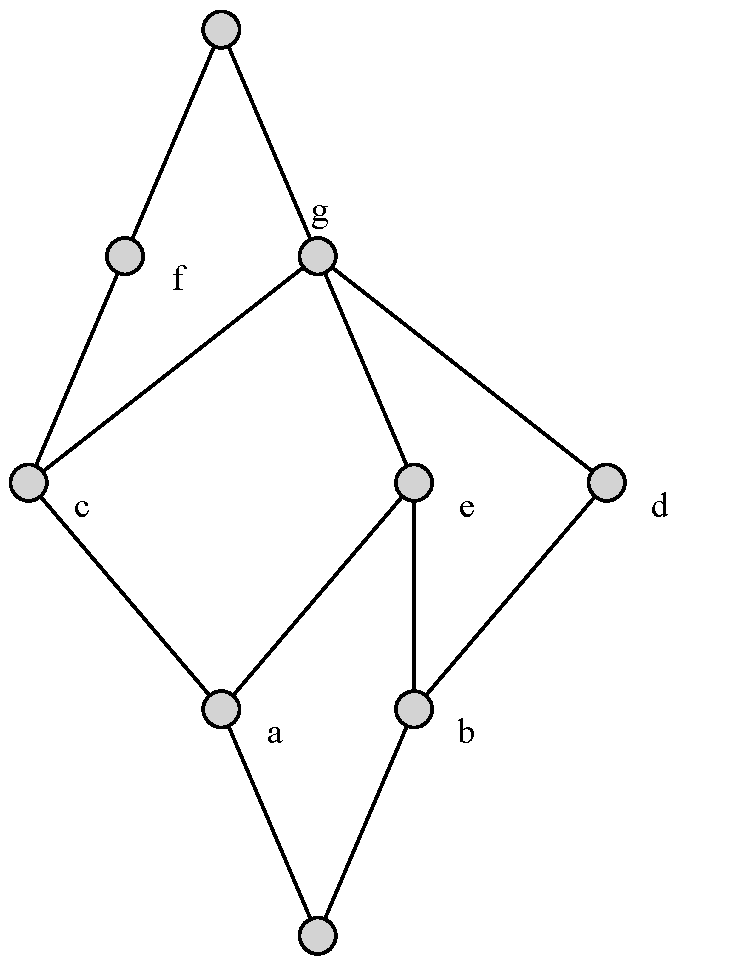
\includegraphics[scale=0.5]{images/graphviz(4).pdf}
}
\caption{Tabla del contexto con un retículo de conceptos isomorfo al representado por el diagrama de la derecha.}
\label{tab:my-table}
\end{figure}


Como veremos a continuación, justo este retículo coincide con el del ejemplo de los monumentos de Granada.
    


\section{Representación gráfica de un retículo de conceptos}

\subsection{Diagrama de líneas} 

Según Ganter \cite{ganter_formal_1999} un diagrama de líneas o diagrama de Hasse corresponde a un contexto $(G,M,I) $ si y solo si se cumplen estas 4 cosas:

\begin{enumerate}
    \item El diagrama corresponde al de un retículo bien definido.
    \item Exactamente un nodo $\gamma(g)$ está etiquetado por cada $g \in \G$.
    \item Exactamente un nodo $\mu(m)$ está etiquetado por cada atributo $ m \in \M$.
    \item   $\forall g \in \G, \ \forall m \in \M $ se tiene que $gIm \Longleftrightarrow \gamma(g) \leq \mu(m)$.
\end{enumerate}


Este diagrama de líneas se puede utilizar para leer la extensión o intensión de un concepto, se pueden seguir las aristas representadas por la jerarquía de sub y superconceptos en el diagrama de líneas. La extensión de un concepto puede obtenerse uniendo todos los objetos situados en el círculo respectivo y los círculos a los que se puede llegar por caminos descendentes desde este. Por otro lado, la intensión de un concepto puede obtenerse uniendo todos los objetos situados en el círculo respectivo y los círculos a los que se puede llegar por caminos ascendentes desde este.

En las figuras \ref{fig:comerciales} y \ref{diagramamonuments} se pueden observar los diagramas de líneas de los retículos correspondiente a nuestros ejemplos \ref{ejemplocomerciales} y \ref{monuments} respectivamente: 

\begin{figure}[H]
\begin{center}
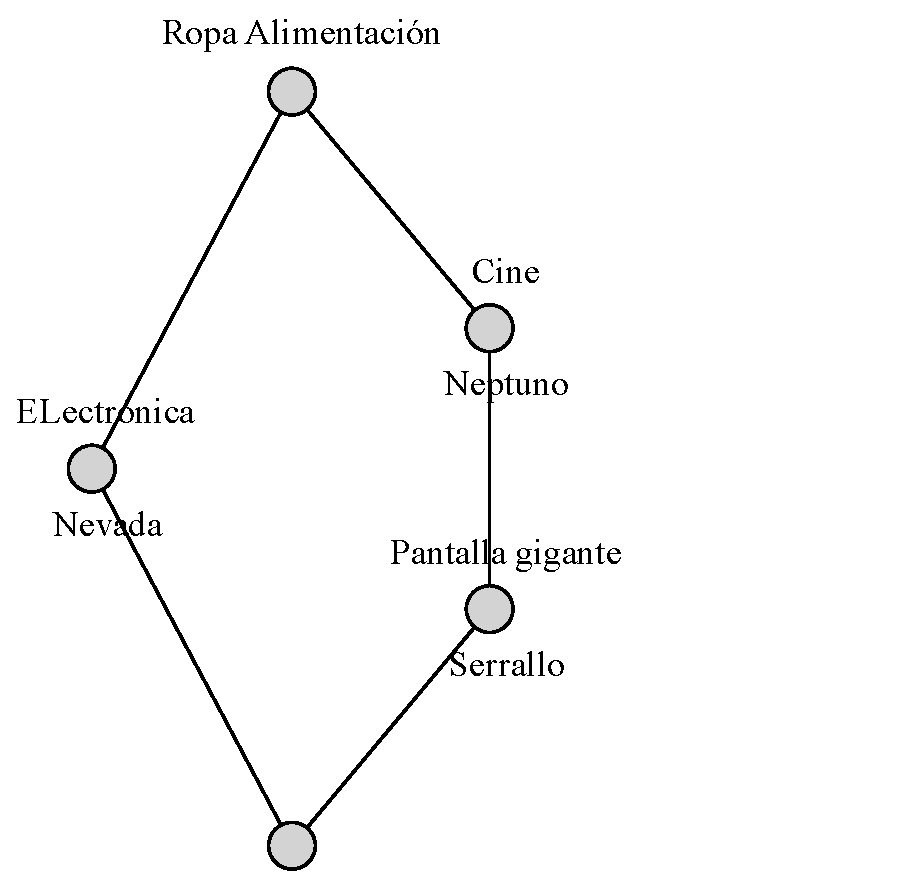
\includegraphics[scale=0.7]{images/graphvizcomerciales.pdf}
\caption{Diagrama de Hasse del retículo de conceptos asociado al ejemplo de centros comerciales de Granada.}
\label{fig:comerciales}
\end{center}
\end{figure}

\begin{figure}[H]
\begin{center}
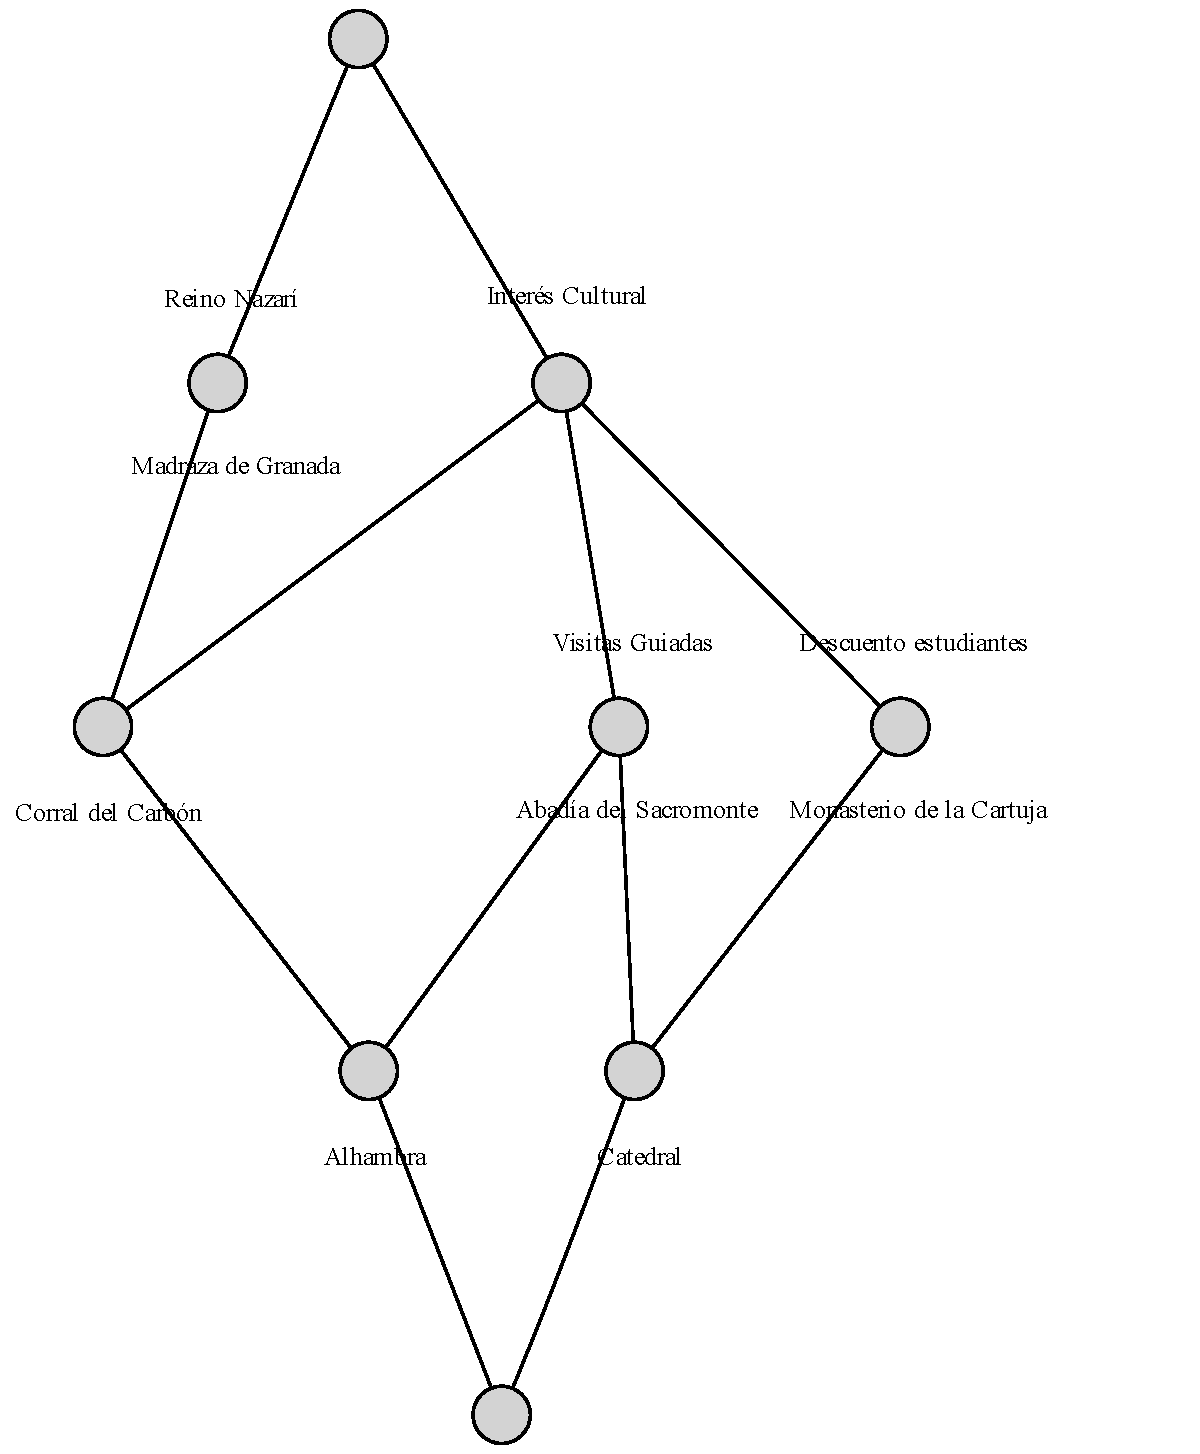
\includegraphics[scale=0.7]{images/graphviz(2).pdf}
\caption{Diagrama de Hasse del retículo de conceptos asociado al ejemplo de monumentos de Granada.}
\label{diagramamonuments}
\end{center}
\end{figure}


Es decir para el concepto que representa los monumentos de con visitas guiadas nos iríamos en la figura \ref{diagramamonuments} al nodo con etiqueta ``Visitas Guiadas'', para leer la extensión del concepto bajamos en los nodos descendientes y nos quedamos con las etiquetas correspondientes de cada uno de ellos. Por lo que la extensión sería \{Abadía del Sacromonte, Alhambra, Catedral\}, y la intensión se leería ascendiendo desde ese nodo y tomando las etiquetas de los atributos, en este caso la intensión sería \{Interés Cultural, Visitas Guiadas\}, dando lugar al concepto (\{Abadía del Sacromonte, Alhambra, Catedral\},\{Interés Cultural, Visitas Guiadas\}).

En este retículo, según el diagrama, el elemento unidad o $0_{\mathfrak{B}}$ sería (\{$\emptyset$\},\{Reino Nazarí, Visitas Guiadas, Descuento Estudiantes,Interés Cultural\}).

\subsection{Implicaciones}

Uno de los resultados adicionales que proporciona el FCA, además del retículo de conceptos, es un conjunto de implicaciones entre atributos. Estas implicaciones provocan que el FCA se use para ciertas aplicaciones que requieran estudiar las dependencias entre los atributos de los datos. 

\begin{definition}[Implicación \cite{ganter_formal_1999}]
Sea $\M$ un conjunto de atributos de un contexto formal $(\G,\M,\I)$, y sean $C,D \subseteq M$. Diremos que $C \to D$ es una implicación que se cumple en $(\G,\M,\I)$ si cada objeto que tiene todos los atributos de $C$ tiene también todos los atributos de $D.$
\end{definition}

\begin{proposition}\cite{ganter_formal_1999}
Una implicación $C \to D$ se cumple en $(\G,\M,\I) \Longleftrightarrow D \subseteq C''$.
\end{proposition}

 Para leer implicaciones a partir de un diagrama, se elige un conjunto de atributos y se toman los conceptos correspondientes a ellos, a partir de los cuales se construye el ínfimo de dichos conceptos. Los  atributos  que  están  por encima  del  concepto  identificado por el ínfimo están implicados por los atributos previamente elegidos. 

Así en nuestro ejemplo tendríamos implicaciones como \{Visitas Guiadas, Descuento Estudiantes\} $\to$ \{Interés Cultural \}. En efecto, \{Interés Cultural\} $\subseteq $ \{Visitas Guiadas, Descuento Estudiantes\}=\{Catedral\}$'$ =\{Interés Cultural, Visitas Guiadas, Descuento Estudiantes\}.


\section{Software para la generación de conceptos y dibujo del retículo}

Aunque posteriormente realizaremos una implementación propia de los principales algoritmos propuestos a lo largo de la historia para la generación de conceptos, ya hay algunos programas que implementan algunos algoritmos en concreto o que dibujan el retículo de conceptos. Estos son algunos de ellos:

\begin{itemize}

    \item El primer programa desarrollado para trabajar con FCA fue \textit{GLAD} \cite{glad}.  Implementa diversos algoritmos para el minado de conceptos pero está muy limitado a conceptos con un número reducido de atributos.
    
    \item Una de las herramientas más usadas es el programa Concept Explorer (ConExp) \cite{concept-explorersoftware}, este posee las características esenciales para trabajar con el FCA. Proporciona minado de conceptos, construcción del retículo y su representación gráfica, incluso minado de implicaciones. Es una herramienta de software libre implementada en Java. Su sitio web se puede consultar aquí \href{http://conexp.sourceforge.net/index.html}{ConExp} \footnote{http://conexp.sourceforge.net/index.html}.
    
    \item \textit{TOSCANAJ} \cite{toscana} es otra herramienta algo más avanzada para el procesamiento de conceptos. También implementada en Java. Su característica principal es que posee una interfaz para utilizar bases de datos mediante el FCA.
    
    \item Otro software libre implementado en Java es \textit{GALICIA} \cite{galicia}. Destaca por su interfaz gráfica de fácil acceso y la posibilidad de realizar test de nuevos algoritmos para la construcción de los retículos.
    
    
    \item Otra herramienta muy útil para trabajar con el FCA es la librería \textit{CONCEPTS} para Python. La documentación de esta librería la podemos encontrar en su \href{https://concepts.readthedocs.io/en/stable/}{ página web} \footnote{https://concepts.readthedocs.io/en/stable/}. Es la que se ha utilizado en este trabajo para la representación gráfica de los retículos, está basada en el uso de \textit{GRAPHVIZ} \cite{graphviz}.
    
\end{itemize}

Una lista actualizada y mucho más extensa de todo el software disponible para trabajar con el FCA la podemos encontrar en su \href{https://upriss.github.io/fca/fcasoftware.html}{sitio web} \footnote{https://upriss.github.io/fca/fcasoftware.html}. Según el objetivo del trabajo que tengamos nos será más conveniente el uso de un software u otro.

\section{Escenarios de uso del FCA}
 
Ya en la introducción comentábamos algunas de las aplicaciones que posee esta teoría, en esta sección las expondremos con mayor nivel de detalle. 

Una de las principales ventajas del FCA, es que permite trabajar con conjuntos de datos proporcionando una visualización de la estructura que poseen, es por ello que puede ser utilizado de diversas maneras según qué objetivo deseemos conseguir. Al ser una herramienta para analizar datos, así como su estructura, su uso abarca gran variedad de campos relacionados con la clasificación y el análisis de datos. 

En sistemas de recuperación de información y clasificación de documentos\cite{carpineto_lattice_1996}, \cite{lindig_concept-based_nodate} se utiliza el FCA para ordenar el conjunto de documentos en una estructura de retículo de conceptos. Definiendo ciertas características o atributos para los documentos, se puede elaborar una tabla cruzada y construir así dicho retículo. El problema suele estar en que el número de documentos a clasificar suele ser bastante grande, pero a partir de la petición del usuario se puede refinar la exploración del retículo para que no sea tan costoso. Es de gran utilidad ya que generalmente cuando un usuario se encuentra en un documento, los vecinos superiores e inferiores del documento en el retículo serán aquellos que más relación tengan con el documento actual.

En el ámbito de la compilación se puede usar tanto para identificar módulos dentro de un proyecto \cite{modules_fca}, como para tratar la herencia de clases dentro de un proyecto \cite{classhierarchies_fca}. Se estructuran todas las cabeceras de los módulos o de las clases que heredan en forma de retículo y se observa si el retículo tiene una estructura válida y coherente para complementar el proceso de compilación.

O su uso más habitual, en el análisis (o minería) de datos, donde se permite al usuario explorar el conjunto de datos, realizar búsquedas de diferentes tipos sobre el mismo, observar las relaciones que tienen ciertos atributos con sus elementos o refinar los resultados en secciones interesantes. Para este caso los requisitos de los algoritmos pueden ser muy diferentes. Se puede realizar primero la elaboración de la parte del retículo que consume mucho tiempo y luego permitir al usuario realizar otras consultas en la red, esto se conoce como \textit{retículo iceberg} \cite{iceberg}. Por otro lado, se puede hacer una primera búsqueda en la que se almacenan los nodos más importantes y luego se van explorando los necesarios a petición del usuario. 

Estos son unos de los usos más populares del FCA pero hay muchos más ejemplos como los que se pueden consultar en \cite{Ganter}. Todos ellos tienen en común la necesidad de encontrar un algoritmo que calcule el retículo de conceptos, y cualquier algoritmo que se requiera para esta tarea tiene cierta complejidad computacional. Por ello, dedicaremos las siguientes secciones a explorar y comparar los distintos algoritmos que existen para el cálculo del retículo de conceptos, obteniendo una instantánea global de todos ellos y de su desempeño según el ámbito en el que trabajemos.


\chapter{Algoritmos para el FCA}
   \label{chap:4}
Uno de los componentes más importantes de cualquier herramienta que utilice el análisis formal de conceptos es el algoritmo que emplee para extraer todos los conceptos a partir de un determinado contexto. Su eficiencia tanto a nivel de espacio como de tiempo de ejecución, juega un papel crucial en las aplicaciones que se le pretendan dar.

Anteriormente, la mayoría de los algoritmos para el análisis de conceptos formales eran comparados y probados en pequeños conjuntos de datos. Pero con el paso de los años se han desarrollado algoritmos cada vez más sofisticados que, aprovechando ciertas propiedades teóricas del FCA, han mejorado considerablemente el desempeño de los algoritmos más clásicos. Por ello este capítulo está dedicado a la presentación de algunos algoritmos para el Análisis Formal de Conceptos.

\section{Propiedades deseables de un algoritmo}

A la hora de trabajar con un algoritmo para la exploración de conceptos, es importante reflexionar antes acerca de las propiedades óptimas que debe de tener este en referencia a su funcionamiento interno, para de esta manera aprovechar al máximo los recursos disponibles.

Como todo buen algoritmo que se precie, un algoritmo diseñado para esta tarea debe de cumplir con ciertas propiedades básicas como que sea finito, preciso, escalable y eficiente. Pero restringiéndonos a nuestro problema, la propiedad que más nos interesa, y en la que más nos vamos a centrar, es la eficiencia, y cuando hablamos de eficiencia nos referimos a dos tipos de eficiencia. Buscamos que sea eficiente en tiempo y eficiente en espacio (aunque este trabajo está enfocado en el análsis de la eficiencia en tiempo). El estudio comparativo que veremos en la próxima sección estará centrado en ella, ya que como comentábamos en capítulos anteriores el principal uso del FCA es aportar utilidad mediante el tratamiento y la comprensión de conjuntos de datos complejos, y para ello la eficiencia es una propiedad clave. Estará determinada en gran parte en cómo enfoca el algoritmo el cálculo de todos los conceptos del retículo. Sin olvidar, como hemos mencionado, que no se dejen de lado las propiedades básicas. Debe ser finito, es decir, que esté diseñado para que se termine en un objetivo determinado, en este caso el retículo de conceptos. También debe ser preciso, hay que dejar claro qué se calcula y cómo, sin posibilidad de errores. Y, por otro lado, la escalabilidad que en nuestro caso particular es una propiedad muy interesante ya que puede resultarnos muy beneficioso que el algoritmo se comporte de igual o mejor manera conforme el conjunto de datos que recibe como entrada crece. 

Además, teniendo en cuenta que el proceso de generar un retículo es algo iterativo, y puede verse como un desarrollo o expansión de nodos hasta completar el grafo (retículo), lo que particularmente nos gustaría que cumpliese el algoritmo es que se calcule cada punto del espacio de búsqueda tan solo una sola vez. Esta idea es algo  a lo que los primeros algoritmos no daban mucha importancia. Se repetía el mismo proceso iterativo sin tener en cuenta que se recalculaban los mismos conceptos la mayoría de las veces, ya que al expandir los conceptos de la base del grafo, muchos de los conceptos generados tienen en común varios sucesores. La repetición de conceptos es una de las características principales en las que se centraron los autores a la hora de desarrollar nuevos algoritmos, llegando a añadir atributos a los conceptos para marcar si ya se había explorado o no. Como es lógico el buen uso de esta técnica debe repercutir directamente en la eficiencia del algoritmo. Se necesitará menos espacio para su ejecución y se calcularán antes el resto de conceptos. 



\section{Presentación de los algoritmos}\label{alg}

Desde los comienzos del FCA, se han publicado conocidos algoritmos para la tarea de la generación del retículo de conceptos; el primero fue el que Ganter\cite{Ganter} propuso en 1984, y a partir de ahí muchos otros surgieron intentando mejorar o modificar el trabajo que existía hasta la fecha.

A lo largo de la literatura, si recopilamos todos los algoritmos propuestos, se puede observar una principal diferencia entre ellos que va a dar lugar a dos grandes grupos: distinguiremos entre aquellos que ante un cambio en el conjunto de datos de entrada deben de volver a calcular todo el retículo de conceptos y los algoritmos que, por otro lado, solo deben modificar el retículo ya existente para añadir los nuevos cambios.

Generalmente esta caracterización establece una clasificación entre lo que conocemos como algoritmos por lotes\footnote{o algoritmos tipo \textit{batch}} y algoritmos incrementales. Los algoritmos por lotes comienzan siempre por un conjunto de datos y a partir de ahí construyen de manera secuencial todo el retículo de principio a fin, sin posibilidad a interrumpir o modificar este proceso. Por otro lado los incrementales se caracterizan por manejar una estructura de base, que en este caso será un retículo, sobre la que se realizan actualizaciones para llegar al resultado final. 

La principal desventaja de los algoritmos por lotes mencionados anteriormente es que, como ya hemos explicado, requieren la elaboración del retículo por completo desde el principio. Por ello, en el caso de que la base de datos cambie, es necesario que todo el retículo se construya nuevamente desde cero, lo que puede resultar muy ineficiente para ciertas aplicaciones como puede ser en la recuperación de información. Por ejemplo si disponemos de una base de datos de documentos, y usamos el FCA para recuperarlos, si es frecuente que se indexen nuevos documentos, necesitaremos estar construyendo todo el retículo cada poco tiempo. Dentro del enfoque por lotes los más destacables son el algoritmo de Lindig \cite{lindig_concept-based_nodate}, el InClose \cite{inclose}, el algoritmo de Bordat \cite{bordat_calcul_nodate} y el propuesto por Berry \cite{berry}.

En cambio, los algoritmos incrementales resuelven este problema utilizando la estructura del retículo como entrada para ir actualizando el mismo. Los enfoques incrementales más populares son el de Norris\cite{norris_algorithm_1978}, Dowling \cite{dowling_irredundant_1993}, Godin \cite{godin_incremental_1995}, Capineto y Romano \cite{carpineto_lattice_1996} y AddIntent \cite{addintent}. 

Es por ello que es muy importante que la elección del algoritmo que tomemos sea en función de la aplicación que se le va a dar y de la topología de los datos con los que se va a tratar. Ante aplicaciones con constantes cambios en los datos quizás nos interese más optar por un algoritmo incremental. Aunque como discutiremos en el análisis experimental, esto variará mucho en función de la distribución de los datos con los que estemos tratando y el algoritmo elegido.


\section{Revisión bibliográfica de algoritmos}

A lo largo de la literatura se han presentado muchos algoritmos dedicados a la tarea de construir el retículo de conceptos. En la próxima sección presentaremos los elegidos y analizados en este trabajo, pero antes es necesario realizar una reflexión sobre algunos enfoques que son bastante populares pero que no se han incluido en este estudio por diversos motivos.

Uno de los algoritmos más antiguos que se encuentran en la literatura es el de Dowling \cite{dowling_irredundant_1993} pero no lo hemos incluido ya que el pseudocódigo que aporta el autor en el documento es prácticamente ilegible y el artículo original en el que se presenta está en francés, lo que ha dificultado aún más su comprensión.

Nourine y Raynaud \cite{nourine} presentaron un algoritmo incremental para la construcción del retículo de conceptos. Este algoritmo en estudios previos sobre la materia obtuvo un rendimiento muy bajo, bastante peor que el del resto de algoritmos, por este motivo no hemos considerado necesario volver a implementarlo. Lo mismo ocurre con el algoritmo de Valtchev \cite{valtchev_partition-based_2002}, el de Gajdos \cite{gajdos_new_nodate} y el propuesto en $1999$ por Carpineto y Romano \cite{carpineto_lattice_1996} (este último ya lo descartan algunos autores en sus comparativas).

Otro algoritmo con un desempeño muy malo en anteriores trabajos es el de Chein \cite{chein}, que además fue uno de los primeros en la literatura. Este algoritmo se usa como base para construir otro que es bastante popular como es el algoritmo Close-By-one \cite{close-by-one}, pero como veremos en la siguiente sección, se ha optado por implementar una mejora que surgió de ese algoritmo y fue publicada después de realizar las otras comparativas. El hecho de implementar un algoritmo que surge como la mejora de estos dos últimos algoritmos nos ha hecho descartar ambos para el estudio y quedarnos con la versión más óptima de ellos. 


Por otro lado, durante la revisión bibliográfica también se recopilaron diversos algoritmos que construyen el retículo de conceptos utilizando técnicas de paralelización. Un ejemplo de estos son:  el algoritmo propuesto por Olga Prokasheva \cite{mapreduce} que utiliza el modelo MapReduce para la construcción del retículo, o el algoritmo de recursión paralelo propuesto por Krajca \cite{paralel}. Su implementación se ha descartado debido a que no sería justo comparar algoritmos secuenciales con paralelizables para la misma tarea, pero sería una vía de trabajo futuro interesante el repetir este trabajo con algoritmos paralelizables.

\section{Algoritmos por lotes}


Los algoritmos por lotes para el Análisis Formal de Conceptos son aquellos que construyen el retículo de conceptos partiendo desde el inicio de manera secuencial, y que ante algún cambio en el conjunto de datos deben volver a construir el retículo por completo. En esta sección veremos los más populares y sobre qué principios se basa su funcionamiento.

Para obtener una idea más clara del funcionamiento de los algoritmos, en algunas ocasiones haremos referencia al ejemplo sencillo de los centros comerciales de Granada, cuyo contexto recordemos que era:

\begin{table}[H]
\centering
\resizebox{15.9cm}{!}{
\begin{tabular}{|l|l|l|l|l|l|}
\hline
$\I$                   & \textbf{Cine(C)} & \textbf{Ropa(R)} & \textbf{Alimentación(A)} & \textbf{Pantalla Gigante(P)} & \textbf{Electrónica(E)} \\ \hline
\textbf{Nevada (NA)}   &               & x             & x                     &     &x                   \\ \hline
\textbf{Neptuno (NE)}  & x             & x             & x                     &       &                    \\ \hline
\textbf{Serrallo (SE)} & x             & x             & x                     &     x    &                  \\ \hline
\end{tabular}
}
\caption{Tabla cruzada para un contexto de centros comerciales de Granada.}
\label{tab:comcercialesal}
\end{table}



Comenzaremos por uno de los primeros algoritmos que encontramos en la literatura, a partir del que a base de mejoras y modificaciones se fueron apareciendo el resto.

\subsection{Algoritmo de Ganter}
\label{alg:nextclosue}

En 1984, Ganter \cite{Ganter} diseñó el primer algoritmo en la historia del FCA,  llamado \textit{NextClosure}, basado en la idea de que cada concepto está únicamente determinado por su extensión e intensión.

En primer lugar, Ganter en su estudio apreció que los operadores de derivación eran operadores de clausura:

\begin{definition}[Operador de clausura\cite{Ganter}]

Sea $\mathcal{P}(M)$ el conjunto de todas las partes de $M$. Llamamos operador de clausura \footnote{También conocido como cierre de un conjunto} a una función:

$$ \overline{*} : \mathcal{P}(M) \to \mathcal{P}(M) $$ 

que es extensiva, monótona e idempotente, esto es, para todo $A,B \subseteq M$:

\begin{enumerate}
    \item $A \subseteq \overline{A}$
    \item $A \subseteq B \Longrightarrow \overline{A} \subseteq \overline{B}$
    \item $\overline{\overline{A}} = \overline{A}$
\end{enumerate}
\end{definition}

\begin{definition}[Sistema de clausura\cite{Ganter}]

A la colección de todos los conjuntos cerrados de un operador de clausura se le llama sistema de clausura.

\end{definition}

Si nos remontamos a la Proposición \ref{propositionmonotony}, vemos que los operadores doble prima $<''>$ son operadores de clausura tales que $'':2^{|\G|} \to 2^{|\G|}$ y $'':2^{|\M|}\to2^{|\M|}$. 

Utilizando que por definición $(A,B)$ es un concepto si y solo si $A=B'$ y $B=A'$, si aplicamos dichos operadores $A'' = (A')' = B ' = A$ vemos que todo $A$ que sea la extensión de un concepto formal cumple la definición de conjunto cerrado (análogo para $B''=B$). Concluimos que las extensiones e intensiones que forman un concepto son los sistemas de clausura de los operadores dobles de derivación.

Con este argumento Ganter desarrolló un algoritmo cuyo objetivo era partir del conjunto de objetos más pequeño de todos, e ir calculando el cierre de cada conjunto para así obtener todas las extensiones de los conceptos existentes. Las intensiones vendrían unívocamente determinadas por dichas extensiones. Pero para ordenar los subconjuntos de objetos y de atributos necesitó establecer el orden lexicográfico.

\begin{definition}[Orden lexicográfico\cite{Ganter}]
Sea $M=\{1,2,...,m\}$ un conjunto ordenado linealmente. Sean $A,B\subseteq M$, con $A=\{a_1,...,a_j\}$, $B=\{b_1,...,b_k\}$ definimos:

$$A<B \Longleftrightarrow (a_1 < b_1) \vee (a_1= b_1 \wedge \{a_2,...,a_j\} < \{b_2,...,b_k\}) $$
\end{definition}

Así siendo $A=\{1,2,3\}$ y $B=\{2,3,5\}$, se tendría $A<B$.

Siguiendo este orden el algoritmo comienza examinando el conjunto formado por el mayor objeto de $\G$ , y termina cuando el cierre generado canónicamente es igual a $\G$, esto es $A''=\G$.  Y en cada iteración calcula el cierre de la extensión formada $A$, y comprueba si es la extensión de un concepto. En cuyo caso añade el concepto $(A'',A')$. Para la implementación cogeremos la versión del algoritmo que implementó Sergei Obiedkov en su artículo, veamos su pseudocódigo \cite{comparingperformance}:

\begin{algorithm}[H]
\caption{Pseudocódico del algoritmo \textit{NEXTCLOSURE}.}
\label{code:nextlcosure}
     \KwIn{Un contexto$(\G,\M,\I)$}
     \KwOut{Un retículo de conceptos $L$}
     $g:=max (\G)$\\
     $L:=\emptyset$\\
     $A:=\emptyset$\\
     \While{$A \neq \G$}{
     $A:=A \cup \{g\}\setminus\{h|h \in A \& g<h\}$\\
     \If{$\{h | h \in A''\setminus A \& h < g\}==\emptyset$}{
     $L:= L \cup \{(A'',A')\}$\\
     $g:=max(\{h |h\in G \setminus A''\})$\\
     $A:=A''$
     }\Else{
     $g:=max(\{h|h \in \G\setminus A\& h<g\})$
     }
     }
     \textbf{return} $L$;
     
\end{algorithm}

Para mejorar su rendimiento, vemos que al principio (algoritmo \ref{code:nextlcosure} - línea 6) Ganter incluyó una condición para comprobar si el cierre que se iba a calcular estaba ya dentro de la lista de conceptos, y así evitar calcularlo nuevamente. Es lo que se conoce como test de canonicidad.

\begin{definition}[Canonicidad \cite{Ganter}]
Sea A un subconjunto de $\G$, y $g \in \G$. La generación de $A''$ se considera canónica si $A''\setminus A$ no contiene a $g$.
\end{definition}

 Bajo estas condiciones, suponiendo que la generación de $A''$ es canónica (y $A''$ no es igual a $\G$), el siguiente conjunto a examinar se obtiene a partir de $A''$ como sigue:

$$A''\cup \{g\} \setminus \{h | h \in A'' \ \& \ g < h\} \ \ con \ g=max(\{h | h\in \G \setminus A''\})$$

Si por el contrario no es canónica el siguiente conjunto a examinar se consigue de una manera similar, pero el objeto a añadir debe de ser menor que el mayor de $A$:

$$A\cup \{g\} \setminus \{h | h \in A \  \& \ g < h\} \ \ con \ g=max(\{h | h\in \G \setminus A \ \& \ h < max(A)\})$$

Este algoritmo propuesto por Ganter tiene una eficiencia teórica de $O(|\m{G}|^2 \times |\m{M}| \times |L(\m{G},\m{M},\m{I})|)$ \cite{comparingperformance}.

Aplicando el algoritmo a nuestro ejemplo \ref{tab:comcercialesal}, obtendríamos la siguiente traza y su correspondiente salida:

\begin{table}[H]

\resizebox{16.0cm}{!} {
\begin{tabular}{|l|l|l|l|l|l|}
\hline
\textbf{Iteración} & \textbf{A}  & \textbf{\{g\}} & \textbf{(A'',A')}        & \textbf{¿Canónica?}       & \textbf{L}                                        \\ \hline
0                  &             &                &                          &                           & add(\{$\emptyset$\},\{C,R,A,P,E\}) \\
1                  & $\emptyset$ & \{SE\}         & $(\{SE\},\{C,R,A,P\})$   & Sí, A=\{SE\},g=NE     & add($\{SE\},\{C,R,A,P\})$                         \\
2                  & \{SE\}      & \{NE\}         & $(\{NE,SE\},\{C,R,A\})$  & Sí, A=\{NE,SE\}, g=NA & add($(\{NE,SE\},\{C,R,A\})$)                      \\
3                  & \{NE,SE\}   & \{NA\}         & $(\{NA\},\{R,A,E\})$     & Sí, A=\{NA\}, g=SE    & add($(\{NA\},\{R,A,E\})$)                         \\
4                  & \{NA\}      & \{SE\}         & $(\{NA,NE,SE\},\{R,A\})$ & No, A=\{NA\}, g=NE    &                                                   \\
5                  & \{NA\}      & \{NE\}         & $(\{NA,NE,SE\},\{R,A\})$ & Sí, A=\{NA,NE,SE\}        & add($(\{NA,NE,SE\},\{R,A\})$)                     \\ \hline
\end{tabular}
}
\caption{Tabla con el procedimiento del algoritmo NEXTCLOSURE paso a paso.}
\label{tab:my-table}
\end{table}

Vemos que es muy parecida a la traza del primer algoritmo básico que presentamos en la introducción \ref{tab:naive-algorithm}, pero con la diferencia de que gracias al test de canonicidad y a la forma de construcción del siguiente conjunto $A$ a examinar, nos ahorramos muchos cálculos innecesarios.



\subsection{Algoritmo de Lindig}
\label{alg:lindig}

Unos años después Lindig \cite{lindig_concept-based_nodate} presentó otro algoritmo alternativo con una idea diferente. En 1999 presentó un algoritmo tipo $"$\textit{de abajo hacia arriba}$"$ cuya idea era generar el concepto unidad del retículo (que se encuentra más abajo) y recursivamente generar todos los vecinos superiores hasta generar el retículo completo. Para lograr esta tarea utilizó un árbol de conceptos que permite comprobar si un concepto ha sido ya generado anteriormente o no.

La descripción explícita de este árbol no se encuentra en su artículo original, por ello nuestra elección ha sido utilizar una lista de nodos en la que cada nodo posee a su vez otra lista con sus vecinos superiores e inferiores tal y como utilizó Obiedkov \cite{comparingperformance} para su implementación.

Para encontrar todos los vecinos superiores de un concepto e ir generando el retículo, Lindig se basó en la idea que recoge el principal teorema de su artículo \cite{lindig99thesis}. Dado un concepto $(A,B)$ que sea distinto del elemento unidad  \textbf{$1$}$_L$ del retículo, el siguiente conjunto $S$ contiene todos los conceptos mayores que $(A,B)$. 

$$S=\{((A \cup \{g\})'',(A\cup \{g\})') | g \notin A\}$$

Los conceptos del conjunto $S$ son aquellos que son más grandes que $(A,B)$ pero no necesariamente vecinos suyos. Los vecinos superiores los identificamos mediante el siguiente teorema.


\begin{theorem}[Teorema de Lindig \cite{lindig_concept-based_nodate}]\label{th:teoremalindig}

Sea $(A,B)$ $\in \mathcal{B}(\mathcal{G},\mathcal{M},\mathcal{I})$ y $(A,B) \neq$ \textbf{$1$}$_\mathcal{B}$. Entonces $(A \cup \{g\})''$, donde $g \in \G \setminus A$, es una extensión de un vecino superior de $(A,B)$ si y solo si para todo $y \in (A \cup \{g\})'' \setminus A$ se cumple lo siguiente : $(A\cup \{y\})''=(A\cup \{g\})''$. 
\end{theorem}

La prueba de este teorema se puede encontrar en la tesis original de Lindig \cite{lindig99thesis}.

La clave del teorema está en la monotonía del operador $''$, el cual nos asegura que al calcular la extensión de un nuevo concepto, esto es, $A \cup \{g\}$ y calcular su cierre, obtendremos la extensión de un concepto superior al anterior: $A \cup \{g\} \subseteq (A \cup \{g\})''$.

Este es el fundamento del algoritmo \textit{NEIGHBORS} \cite{lindig_concept-based_nodate}, desarrollado por Lindig:

\begin{algorithm}[h]
\caption{Pseudocódico del algoritmo \textit{NEIGHBORS}.}
\label{code:neighbors}
     \KwIn{((A,B), ($\mathcal{G},\mathcal{M},\mathcal{I}$))}
     \KwOut{Lista de vecinos del concepto}
    
    $\text{min} \leftarrow \G \setminus A$\\
    $\text{neighbors} \leftarrow \emptyset$\\
    \For{$ g \in  \mathcal{G}\setminus A$}{
    $M_1 \leftarrow (A \cup \{g\})'$\\
    $G_1 \leftarrow M_1'$ \\
    \If{$(\text{min} \bigcap (G_1 \setminus A \setminus \{g\})) == \emptyset$}{$\text{neighbors} \leftarrow \text{neighbors} \cup \{(G_1,M_1)\}$}
    \Else{$\text{min} \leftarrow \text{min} \setminus \{g\}$}
    
    \textbf{Return} neighbors;
    }
\end{algorithm}

El conjunto \textit{min} se usa para almacenar todos los elementos de $\mathcal{G}\setminus A$ que generan vecinos superiores. Inicialmente se asume que todos los elementos generan vecinos y posteriormente se eliminan aquellos que no generan vecinos. 

Su eficiencia teórica es del orden $O(|\G|^2 \times |\M|)$ \cite{lindig_concept-based_nodate}.

Consideremos el ejemplo de generar todos los vecinos superiores del concepto $(\{NE,SE\}$ $,\{C,R,A\})$. Según el algoritmo \ref{code:neighbors}:

\begin{itemize}
    \item En primer lugar inicializamos $min=\G \setminus A = \{NA\}$ y $neighbors=\emptyset$ (líneas 1 y 2).
    \item ahora para $g \in \G \setminus A = g \in \{NA\}$ (línea 3-13)
    \begin{itemize}
        \item calculamos $M_1=(\{NE,SE\} \cup \{NA\})'=\{R,A\}$ y $G_1=\{R,A\}'=\{NA, NE, SE\}$
        \item entraríamos en el primer condicional (línea 6): $(\text{min} \bigcap (G_1 \setminus A \setminus \{g\}))= NA \cap (\emptyset) == \emptyset$
        \item por tanto $neighbors \leftarrow (\{NA,NE,SE\},\{R,A\})$
    \end{itemize}
    \item se devuelven los vecinos que serían $neighbors \leftarrow (\{NA,NE,SE\},\{R,A\})$
\end{itemize}

Podemos comprobar que esto es correcto con el grafo del retículo \ref{fig:comerciales}.

\begin{figure}[H]
  \centering
  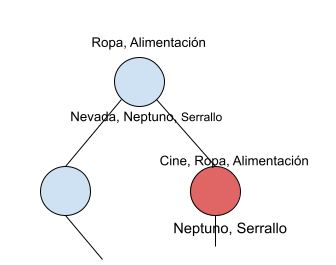
\includegraphics[scale=0.7]{images/grafolindig.png}
  \label{fig:test2}
\caption{Como se comprueba en el grafo el vecino superior del nodo marcado en rojo es $(\{NA,NE,SE\},\{R,A\})$.}
\end{figure}

El algoritmo \textit{NEIGHBORS} se puede usar de forma recursiva para calcular todos los conceptos de un contexto empezando por el más pequeño $(\emptyset, \M)$, dando lugar al algoritmo \textit{LATTICE} \cite{lindig_concept-based_nodate} que nos da el retículo completo. Cada concepto $c$ va a tener dos listas asociadas: la lista de sus vecinos inferiores $x_*$ y la de los vecinos superiores $c^*$. La función \textit{insertLookup} (algoritmo \ref{code:lindig} -línea 4)  se encarga de buscar el concepto $x$ en la lista $L$ de todos los conceptos, y \textit{next} proporciona el siguiente concepto mayor a $c$, usando el orden léxico.

\begin{algorithm}[H]
\caption{Pseudocódigo del algoritmo \textit{LATTICE}.}
\label{code:lindig}
     \KwIn{$(\G,\M,\I)$}
     \KwOut{Retículo de conceptos}
     $c \leftarrow (\emptyset '', \emptyset ')$\\
     $\text{insert}(c,L)$\\
     \For{$x \in \text{Neighbors}(c,(\G,\M,\I))$}{
     \textbf{intentar} $x \leftarrow \text{insertLookup}(x,\L)$\\
    \textbf{en caso de} No encontrar x $ \rightarrow \text{insert}(x,\L)$\\
    $x_* \leftarrow x_* \cup \{c\}$\\
    $c^* \leftarrow c^* \cup \{x\}$}
    \textbf{intentar} $c \leftarrow \text{next}(c,\L)$\\
    \textbf{en caso de} No encontrar c $\rightarrow$ \textbf{exit}
    
    \textbf{return }$\L$

\end{algorithm}

Su eficiencia teórica en el peor de los casos es de $O(|\L| \times |\G|^2 \times |\M|)$ \cite{lindig_concept-based_nodate} ya que las operaciones de búsqueda en la lista no añaden complejidad a lo anterior. Apreciamos que comparte la misma complejidad asintótica que el algoritmo \textit{NEXTCLOSURE} de Ganter.

\subsection{Algoritmo InClose}\label{alg:inclose}

Poco después del algoritmo \textit{NEXTCLOSURE}, Kuznetsov implementó una modificación con el nombre de algoritmo \textit{CLOSE-BY-ONE} \cite{close-by-one}. Ambos tienen en común que en cada iteración trabajan con un concepto actual, a partir del cual van explorando sus vecindades en el grafo.  El siguiente concepto generado es nuevo si su extensión no contiene objetos del concepto actual. Por ejemplo, supongamos que la extensión del objeto actual es \{2\}, si la extensión generada es \{1,2,3\}, el correspondiente objeto no es nuevo y puede ser descartado. 

El algoritmo \textit{IN-CLOSE} propuesto por Andrews \cite{inclose} surge como una mejora del \textit{CLOSE-BY-ONE}. Trata de formar combinaciones de atributos y comprobar si son nuevos o ya han sido generados.

El método general se puede describir de la siguiente manera \cite{inclose}. Se añaden atributos, uno por uno, a la intensión actual. Cada vez que el nuevo atributo se añade, la correspondiente extensión se calcula. Esto se consigue intersecando la extensión actual $A$, junto con la extensión del atributo $\{j\}'$, esto es $A_{new}=A\cap\{j\}'$. Ahora con la nueva extensión hay 3 posibilidades :

\begin{enumerate}
    \item Que sea vacía $A_{new}=\emptyset$.
    \item Que sea no vacía y más pequeña que $A$, $A_{new}\neq\emptyset \subseteq A$.
    \item Que sea el mismo conjunto $A_{new}=A$.
\end{enumerate}
 
Cuando ocurre la opción 3, se finaliza la iteración de los atributos y se corta la recursión de esa rama, es decir, se poda esa rama y evitamos hacer cálculos innecesarios. 
 
Un ejemplo generalizado de este proceso se muestra en \cite{inclose}: para un concepto con intensión $B=\{0,1,3....\}$\footnote{Nótese que no contiene el atributo 2.} ocurriría lo siguiente. Inicialmente se tiene el atributo $\{0\}$, el primer paso sería unir el atributo 1 al 0, como $\{1\} \in B$, $A \cap \{1\}' = A$, obtenemos el caso 3) y se poda esa rama de la recursión (figura \ref{fig:test1}.\textit{(i)} ). Ahora el siguiente es $j=2$ (figura \ref{fig:test1}.\textit{(ii)}, como $2 \notin B$ existen 2 posibilidades, la rama es válida (si $A$ no es vacío), o la rama se poda (si $A$ es vacío). En la figura \ref{fig:test1}.\textit{(iii)} el atributo 3 se une al $\{0,1\}$ y al igual que antes la rama se poda. Así se seguiría con todos los atributos hasta tener el cierre de la intensión $B=\{0,1,3,...\}$.


\begin{figure}[H]
\centering
\begin{minipage}{.6\textwidth}
  \centering
  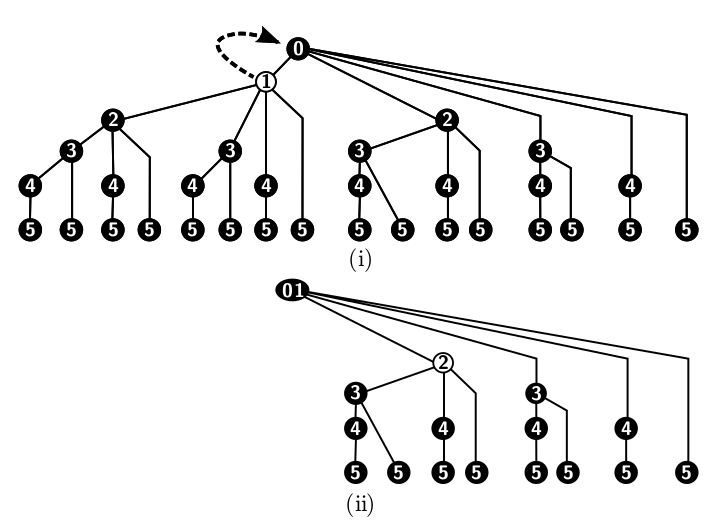
\includegraphics[width=1\linewidth]{images/inclose1.png}

\end{minipage}%
\begin{minipage}{.4\textwidth}
  \centering
  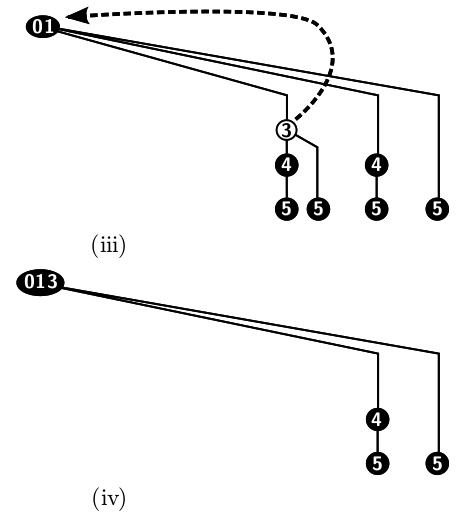
\includegraphics[width=1\linewidth]{images/inclose2.png}

\end{minipage}
\caption{Proceso general de construcción de extensiones del algoritmo InClose (fuente: \cite{inclose}). }
  \label{fig:test1}
\end{figure}

Si nos ceñimos al contexto de la tabla \ref{tab:comcercialesal}, nuestra primera extensión sería $A[0]=\{\G\}=\{NA,NE,SE\}$ y entonces iríamos formando nuevas extensiones iterando sobre $j \in \{\M\}=\{C,R,A,P,E\}$.

\begin{itemize}
    \item En el primer caso $\{j\}=\{C\} \Longrightarrow \{j\}'=\{NE,SE\}$
    \item[] $A[rnew] = A \cap \{j\}'=\{NA,NE,SE\} \cap \{NE,SE\}= \{NE,SE\}$, por lo que estaríamos en el caso 2 ya que hemos obtenido una extensión no vacía distinta de la anterior. 
    \item Aplicaríamos el mismo proceso con cada $\{j\} \in \{C,R,A,P,E\}$ hasta terminar de construir todas las posibles nuevas extensiones de $A$. Si en algún momento obtuviésemos un $A[rnew] =\emptyset$ abandonaríamos esta rama y comenzaríamos la siguiente.
\end{itemize}

Este es el pseudocódigo que modela dicho comportamiento \cite{inclose}.

\begin{algorithm}[H]
\caption{Pseudocódigo del algoritmo \textit{INCLOSE(r,y)}.}
\label{code:inclose}
     \KwIn{lista de extensiones $A_0,...A_r$\\
     lista de intensiones $B_0,...,B_r$\\
     número de concepto actual $r$\\
     número de atributo actual $y$\\
     un contexto formal $(\G,\M,\I)$}
     \KwOut{Modifica los parámetros de entrada: \\
            lista de extensiones $A_0,...A_{rnew}$\\
            lista de intensiones $B_0,...,B_{rnew}$\\
            número del siguiente concepto $r_{new} > r$\\
            número del siguiente atributo $y_{new} > y$}
            
     
     $r_{\text{new}} \leftarrow r_{\text{new}} +1$\\
     \For{$j=y \dots |\M|$}{
     $A[r_{\text{new}}] \leftarrow \emptyset;$\\
     
     \For{$i \ \in \ A[r]$}{
     \If{$I[i][j]$}{$A[r_{\text{new}}] \leftarrow A[r_{\text{new}}] \cup \{i\}$}
     }
     \If{$\abs{A[r_{\text{new}}]} > 0$}{
     \If{$\abs{A[r_{\text{new}}]}=\abs{A[r]}$}{
     $B[r] \leftarrow B[r] \cup \{j\}$}
     }\Else{
     \If{$\text{IsCannonical}(r,j-1)$
     }{
     $B[r_{\text{new}}]\leftarrow B[r] \cup \{j\}$\\
     $\text{InClose}(r_{\text{new}}, j+1)$
     }
     }
     }

\end{algorithm}

La función \textit{ISCANNONICAL} \cite{inclose}, comprueba si el cierre que hemos obtenido ha sido ya generado antes, para evitar hacer cálculos repetidos. Devuelve \textit{true} si no encuentra $A[r_{new}]$ en las extensiones ya calculadas y \textit{false} en caso de haberlo encontrado.  La eficiencia teórica del algoritmo completo es del orden $O(|\G|^2 |\M| |L|)$ \cite{inclose}.

\subsection{Algoritmo de Berry}
\label{alg:berry}


Este algoritmo implementa una búsqueda en profundidad. En primer lugar se calculan los primeros sucesores del elemento unidad y, posteriormente, para cada sucesor, se calcula su cobertura, esto es, todos los conceptos que son sucesores de ese concepto. Berry \cite{berry} realizó las siguientes apreciaciones antes de desarrollar su algoritmo:

\begin{definition}
Sea $(\G,\M,\I)$ un contexto formal, sean $x, y \in \M$. Diremos que $x$ domina a $y$ si $\{x\}' \subseteq \{y\}'$. 
\end{definition}

En la tabla \ref{tab:comcercialesal} podemos observar que, por ejemplo, Pantalla Gigante domina a Cine, puesto que $\{P\}'\subseteq \{C\}'$.

\begin{definition}[Rectángulo máximo \cite{berry}]
Dado un contexto $(\G,\M,\I)$, un rectángulo máximo de $I$ es un conjunto $X$ de atributos tales que $\forall x,y \in X$, $\{x\}'=\{y\}'$ y $\forall z \in (\M-X), \{z\}' \neq X'$. En este caso $X'=\{x\}'$ para cualquier $x \in X \subseteq \M$.
\end{definition}

Un rectángulo máximo de la tabla \ref{tab:comcercialesal} sería $\{R,A\}$. Tenemos que $\{R\}'=\{A\}'$ y $\forall z \in \{C,P,E\}$, con $Z'\neq X'$.

\begin{definition}[Rectángulo máximo no dominante \cite{berry}]
Dados dos rectángulo máximos, $X$ e $Y$, diremos que $X$ domina a $Y$ si $X'\subset Y'$. Un rectángulo máximo $X$ será no dominante si no hay otro rectángulo máximo al que domine.
\end{definition}

En la tabla \ref{tab:comcercialesal},  el rectángulo máximo  que hemos descrito anteriormente será no dominante puesto que no hay otro rectángulo máximo tal que $X' \subseteq Y'$.

Con esta información Berry desarrolló un teorema para calcular las intensiones del cierre de un concepto y así obtener un método para calcular todos sus sucesores.

\begin{theorem}\cite{berry:THEOREM}
Dado un concepto $(A,B), B\cup X$ es la intensión de un concepto que pertenece al cierre de $(A,B)$ si y solo si $X$ es un rectángulo máximo no dominante de $I(A,\M-B)$. En ese caso la extensión de $B\cup X$ es $A \cap  X'$.
\end{theorem}

En nuestro ejemplo, como ya los hemos descrito anteriormente para calcular el cierre del concepto $(\{NE\},\{C,R,A\})$, la intensión del cierre sería $B\cup X=\{C,R,A\}\cup \{P\}$ ya que $X=\{P\}$ es un rectángulo máximo no dominante de la tabla si le quitamos las columnas $C,R,A$ tal y como dice el Teorema. De esta manera la extensión sería $A\cup \{P\}'=\{NE,SE\}$. Y concluimos que el sucesor del concepto  $(\{NE\},\{C,R,A\})$ sería $(\{NE,SE\},\{C,R,A,P\})$.

El principal problema que tiene esta estrategia es que, en conceptos de mayor tamaño, dos o más conceptos pueden compartir sucesores. El principal objetivo de Berry era procesar cada concepto exactamente una vez, para mejorar notablemente la eficiencia del proceso. Para lograr esto utiliza la información de los rectángulos máximos. Cuando un concepto con un rectángulo máximo es procesado, y se generan todos sus sucesores, se almacena esta información para indicar que cualquier concepto que se vuelva a generar con dicho rectángulo máximo no se debe procesar de nuevo. 


Para ello Berry propone el uso de dos estructuras auxiliares que mantengan esta información actualizada para todo el contexto. Estas estructuras son una tabla de dominancia $T$, la cual indica en cada casilla $T(x,y)$ el número de objetos que impiden que el atributo $x$ domine al atributo $y$, en consecuencia el atributo $x$ domina al atributo $y$ si y solo si $T(x,y)=0$. Y un vector $D$, tal que $D(x)$ que indica el número de atributos $y\in \M$ con $T(x,y)=0$, esto es, el número de atributos que domina $x$. Un rectángulo máximo $X$ será no dominante si y solo si $\forall x \in X$ , $D(x)=|X|$. Dando así entonces respuesta a la pregunta: ``¿Cuáles son los rectángulos-máximos no dominantes?
'' con una eficiencia del orden O(n).

Este es el proceso para crear dichas estructuras a partir de un contexto, lo recogemos en el algoritmo \ref{code:tablas}:

\begin{algorithm}[H]
\caption{Inicializar tablas T y D.}
\label{code:tablas}
     \KwIn{Entrada}
     \KwOut{Salida}
     
     \For{$x \in \M$}{
     $D[x] \leftarrow n;$\\
     \For{$y \in \M$}{
     \For{$z \in \G$}{
     \If{$(x,z) \in \I \ and \ (y,z) \notin \I$}{
     \If{$T[x,y] == 0$}{
     $D[x] \leftarrow D[x] -1;$}
     $T[x,y] \leftarrow T[x,y] +1;$
     }
     }
     }
     }

\end{algorithm}

Para el ejemplo de la tabla \ref{tab:comcercialesal}, las tablas T y D serían:

\begin{minipage}{.5\textwidth}
\centering
    \begin{table}[H]
    \begin{tabular}{|l|l|l|l|l|l|}
    \hline
               & \textbf{C} & \textbf{R} & \textbf{A} & \textbf{P} & \textbf{E} \\ \hline
    \textbf{C} & 0          & 1          & 1          & 0          & 1          \\ \hline
    \textbf{R} & 0          & 0          & 0          & 0          & 0          \\ \hline
    \textbf{A} & 0          & 0          & 0          & 0          & 0          \\ \hline
    \textbf{P} & 1          & 2          & 2          & 0          & 1          \\ \hline
    \textbf{E} & 2          & 2          & 2          & 1          & 0          \\ \hline
    \end{tabular}
    \caption{Tabla T con la dominancia de los atributos entre sí aplicada al ejemplo de los centros comerciales.}
    \label{tab:T}
    \end{table}
\end{minipage}%
\begin{minipage}{.5\textwidth}
  \centering
  \begin{table}[H]
    \begin{tabular}{|l|l|l|l|l|}
    \hline
    \textbf{C} & \textbf{R} & \textbf{A} & \textbf{P} & \textbf{E} \\ \hline
    3          & 2          & 2          & 4          & 3          \\ \hline
    \end{tabular}
    \caption{Tabla D con la información sobre la dominancia de cada atributo con respecto al resto aplicada al ejemplo de los centros comerciales.}
    \label{tab:my-table}
    \end{table}
\end{minipage}

Si analizamos estas tablas, la información más valiosa que obtenemos es que $T(x,y)=0 \ \forall x\in \{R,A\}$ lo cual nos dice que $X=\{R,A\}$ dominan al resto de atributos, y en consecuencia es un rectángulo máximo. Ahora como $|X|=2$ y $D(x)=2 \ \forall x \in X$ deducimos que se trata de un rectángulo máximo no dominante. Estas estructuras nos permiten identificar de forma rápida los rectángulos máximos no dominantes de una relación para poder aplicar el algoritmo diseñado por Berry.

Por último, el algoritmo \textit{INHERIT-CONCEPTS} (\ref{code:berry}) \cite{berry} se encarga de calcular los descendientes de un concepto $(A,B)$, e ir actualizando las tablas T y D con la información de la relación $\I$ para explorar únicamente conceptos nuevos.

\begin{algorithm}[H]
\caption{Algoritmo \textit{INHERIT-CONCEPTS}}
\label{code:berry}
     \KwIn{Un contexto $(\G,\M,\I)$\\
     Un concepto $(A \times B)$\\
     Un vector de conceptos marcados $marked$}
     \KwOut{Un retículo de conceptos $\mathcal{L}(\G,\M,\I)$}
     $ Part = \M - A$;\\
     \For{$X \in Part $}{
     $x \in X$;\\
     \If{$D[x]=|X|$}{$ND \leftarrow ND + X$;}
     }
     $NEW \leftarrow ND$
     \For{$x \in NEW$}{
    $A' \leftarrow (A+X);$\\
    $B' \leftarrow (B \cap X')$;\\
    $L.add(\  A' \times B');$\\
    $PREUPDATE(A,X);$\\
    $INHERIT-CONCEPTS(A'\times B', Marked);$\\
    $POSTUPDATE(A,X)$;\\
    $Y \leftarrow X$\\
    $MARKED \leftarrow MARKED\cup X \cup Y$;
    }

\end{algorithm}

Con los algoritmos \textit{PREUPDATE} \cite{berry} y \textit{POSTUPDATE} \cite{berry}, mantenemos la información de las tablas actualizadas. La eficiencia teórica global del algoritmo es del orden $O(|\G||\M|)$ \cite{berry}.


\subsection{Algoritmo de Bordat}
\label{alg:bordat}

Se trata de otro algoritmo tipo ``\textit{de arriba hacia abajo}'', propuesto por Bordat \cite{bordat_calcul_nodate}. Utiliza una estructura de árbol para almacenar y recuperar los conceptos. La versión del algoritmo que hemos implementado la podemos encontrar en \cite{comparingperformance} y utiliza una función \textit{FIND} que busca si un concepto ha sido generado con una eficiencia de O($|\M|$). Bordat elaboró una proposición con la que fue capaz de describir los elementos que existen alrededor de un concepto para así desarrollar el algoritmo que calcula los vecinos de un concepto \cite{bordat_calcul_nodate}:

\begin{proposition}
Si $(S,T)$ es un predecesor de $(E,F)$ en el árbol, $(X,Y)$ es hermano de $(S,T)$ en el árbol, y $(V,W)$ es el padre de $(S,T)$ y $(X,Y)$ en el árbol, entonces $F \cap Y = W$.
\end{proposition}

En el caso del ejemplo \ref{tab:comcercialesal}, esta proposición describe prácticamente todo el retículo. Sea $(S,T)=(\{NE\},\{C,R,A\})$ un predecesor de $(E,F)= (\{SE\},\{C,R,A,P\})$ tal y como se puede apreciar en el grafo \ref{fig:comerciales}. Tenemos que su hermano izquierdo es $(X,Y)=(\{NA\},\{R,A,E\})$, y su padre es $(V,W)=(\{NA,NE,SE\},\{R,A\})$, con $F \cap Y = \{C,R,A,P\}\cap \{R,A,E\}=\{R,A\}=W$ tal y como nos indica la proposición anterior. 

En esto se basa el algoritmo \textit{LOWER-NEIGHBORS} \cite{comparingperformance} para calcular los vecinos inferiores de un concepto. 

\begin{algorithm}[H]
\caption{Algoritmo \textit{LOWER-NEIGHBORS}}
\label{code:lowerneighbors}
     \KwIn{Un concepto $(A,B)$}
     \KwOut{Lista de conceptos vecinos}
     $ Lattice := \emptyset$;\\
     $C:= B$\\
     $g:=$primer objeto en $A$ tal que $\neg(\{g\}' \subseteq C) $;\\
     si no existe dicho primer objeto, $g$ es el último elemento de $A$\\
     \While{$g!=$último elemento de $A$}{
     $E:=\{g\}$\\
     $F:=\{g\}'$\\
     $h:=g$\\
     \While{$h!=$último elemento de $A$}{
     $h.next()$\\
     \If{$\neg (F \cap \{h\}'\subseteq C)$}{
     $E:=E \cup \{h\}$\\
     $F:=F \cap \{h\}'$}
     \If{$F\cap C=B$}{$Lattice:=Lattice \cup \{(E,F)\}$}
     $C:=C\cup F$
     }
     }

\end{algorithm}

Y con esta idea, partiendo del concepto total $(\{\G\},\{\G\}')$, el algoritmo de \textit{BORDAT} \cite{comparingperformance} calcula el retículo completo:

\begin{algorithm}[H]
\caption{Algoritmo \textit{BORDAT}}
\label{code:bordat}
     \KwIn{Un concepto $(A,B)$  y una extensión  $C$}
     \KwOut{Retículo de conceptos $L$}
     $L=L\cup \{(A,B)\}$\\
     $LN:=LowerNeightbors((A,B))$\\
     
     \For{$(D,E) \in LN$}{
     \If{$C\cap E=B$}{
     $C:=C \cup E$\\
     Bordat(($(D,E),C)$}
     }


\end{algorithm}
Como cada concepto puede ser procesado solo una vez, la complejidad del algoritmo de Bordat es de O(|$\G$||$\M^2$||L|), donde |L| es el tamaño del retículo.

Usaremos el contexto de la tabla \ref{tab:comcercialesal} para ilustrar como funciona el algoritmo \ref{code:bordat}. Partimos del objeto total que es $(\G,\{\G\}')=(\{NA,NE,SE\},\{R,A\})$, $C_0=\{R,A\}$ es la intensión actual. Los siguientes pasos son:

\begin{itemize}
    \item $(\{NA,NE,SE\},\{R,A\})$ es el concepto maximal
    \item $C_0=\{R,A\}$
    \item Se llama a Bordat($\{NA,NE,SE\},\{R,A\}$,$\{R,A\}$)
    \item $(\{NA\},\{R,A,E\})$ , $(\{NE,SE\},\{C,R,A\})$ son los vecinos\\
    inferiores de $(\{NA,NE,SE\},\{R,A\})$
    \item $C_0 \cap \{R,A,E\} =\emptyset \Longrightarrow C_1 =\{R,A,E\}$
    \item Se llama a Bordat($\{NA\}$,$\{R,A,E\}$,$\{R,A,E\}$)
    \item $(\{NA\},\{R,A,E\})$ no tiene vecinos inferiores
    \item $C_1 \cap \{C,R,A\}= \{R,A\} \Longrightarrow C_2 = \{C,R,A,E\}$
    \item Se llama a Bordat($\{NE,SE\},\{C,R,A\}$,$\{C,R,A,E\}$)
    \item $(\{SE\},\{C,R,A,P\})$ es el vecino inferior de $(\{NA\},\{R,A,E\})$
    \item $C_3=\{C,R,A,P,E\}$
    \item Se llama a Bordat($\{SE\},\{C,R,A,P\}$,$\{C,R,A,P,E\}$)
    \item $(\{SE\},\{C,R,A,P\})$ no tiene vecinos inferiores
    \item Se añade el concepto unidad $(\{M\}',\{M\})$=$(\{\emptyset\},\{C,R,A,P,E\})$
    \item Fin del proceso.
\end{itemize}

\section{Algoritmos incrementales}

Por otro lado tenemos los algoritmos incrementales que ante una inserción de objetos en el conjunto de datos solo deben procesar esa modificación en el retículo ya existente y no construir todo el retículo desde el inicio.

Es evidente que con este tipo de algoritmos también se puede construir el retículo completo, simplemente añadiendo objetos desde el inicio hasta tenerlos todos dentro del retículo. Este método será el que utilizaremos para establecer una comparación con los algoritmos por lotes anteriormente explicados. Tendremos una función diferente para cada algoritmo cuya sintaxis será de la forma $AddX(object,Lattice)$ cuyo cometido será el añadir el objeto $"object"$ al retículo $Lattice$. Y así si llamamos a dicha función para todos los objetos de $\G$ de manera incremental podemos construir el retículo completo utilizando un procedimiento muy similar a este que mostramos a continuación.

\begin{algorithm}[H]
\caption{Algoritmo \textit{CREATELATTICE}}
\label{code:createlattice}
     \KwIn{Un contexto $(\G,\M,\I)$\\
     Un retículo de conceptos $L$\\
     Un objeto $g\in \G$ a añadir}
     \KwOut{Retículo de conceptos $L$.}
     
     \For{$g \in \G$}{
     $Add(g,L)$;}
     
     $L$ es el retículo de conceptos
\end{algorithm}

Para simplificar el proceso de creación incremental de los retículos, para todos ellos el concepto correspondiente al elemento unidad \textbf{$0$}$_L$ del retículo $(\{\M\}',\{\M\})$ se añade de manera manual al finalizar cada algoritmo.


\subsection{Algoritmo de Norris}
\label{alg:norris}


El algoritmo propuesto por Norris \cite{norris_algorithm_1978} se puede entender como una versión incremental del algoritmo \textit{CLOSE-BY-ONE} \cite{close-by-one}. El árbol de conceptos se puede construir de la siguiente manera: primero, solo está la raíz del árbol $(\{\emptyset\},\{\emptyset\})$; después se examinan los objetos de $\G$ y para cada cada concepto del árbol se comprueba si el objeto en cuestión tiene todos los atributos de la intensión del concepto; si los tiene, se añade a la extensión; en caso contrario, se crea un nuevo nodo en el árbol y se marca como el hijo del nodo actual, la extensión será la extensión actual más el objeto que está seleccionado; y la intensión será la intersección de la intensión del objeto actual con la intensión del padre, después se pasa al siguiente objeto hasta recorrer $\G$.

Ilustremos esto con el contexto de la tabla \ref{tab:comcercialesal}. Partimos del árbol que solo contiene la raíz trivial, y queremos añadir el primer objeto $g \in \G$, $g=NA$. Tenemos que recorrer todos los conceptos del árbol pero en este primer caso no tenemos ningún concepto. Como el conjunto \{$h | h\in \G  \ \&  h \text{ ya ha sido añadido al retículo} \ \& \{g\}'\subseteq \{h\}'$\} es vacío se añadiría el primer concepto $(\{NA\},\{R,A,E\})$. 

\begin{figure}[H]
  \centering
  
\includegraphics[scale=0.7]{images/paso1norris.pdf}
  \label{fig:test2}
\caption{Retículo tras añadir el primer objeto $\{g\}=\{NA\}$.}
\end{figure}

Ya tendríamos la raíz del árbol que sería $(\{NA\},\{R,A,E\})$. Ahora queremos añadir el objeto $\{NE\}$. Tenemos $(A,B)=(\{NA\},\{R,A,E\}) \in L$. Como $\{R,A,E\} \nsubseteq \{C,R,A\}=\{NE\}'$ se crea un nuevo nodo en el árbol cuya extensión será $\{NA,NE\}$ y la intensión será $\{R,A\} =\{R,A,E\} \cap \{C,R,A\}$, además, al igual que antes se añade el nodo $(\{g\},\{g\}')=(\{NE\},\{C,R,A\})$ y se marca como hijo del anterior. 

\begin{figure}[H]
  \centering
  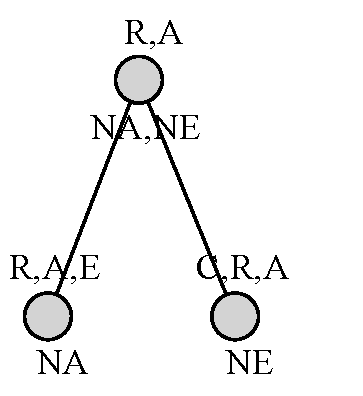
\includegraphics[scale=0.7]{images/paso2norris.pdf}
  \label{fig:test2}
\caption{Retículo tras añadir el objeto $\{g\}=\{NE\}$.}
\end{figure}

Para añadir $\{SE\}$ se actuaría de la misma manera. Recorrer la lista de conceptos para comprobar si debemos modificar su extensión e intensión y añadir el nodo $(\{SE\},\{C,R,A,P\})$.

\begin{figure}[H]
  \centering
  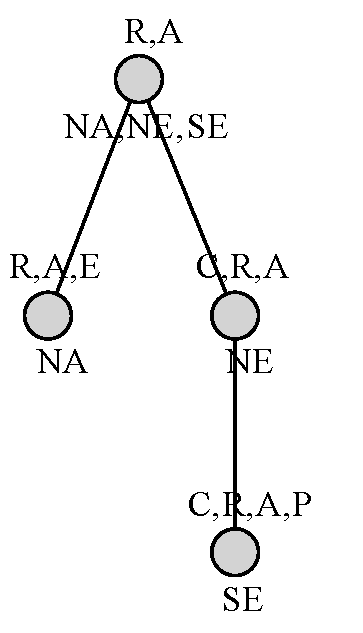
\includegraphics[scale=0.7]{images/paso3norris.pdf}
  \label{fig:test2}
\caption{Retículo tras añadir el objeto $\{g\}=\{SE\}$.}
\end{figure}

Para terminar la construcción del retículo se añade el concepto correspondiente al elemento nulo del retículo $(\{\M\}',\{\M\})= (\{\emptyset\},\{\M\})$.

El pseudocódigo \cite{comparingperformance} que modela este comportamiento es el siguiente (algoritmo \ref{code:norris}) :

\begin{algorithm}[H]
\caption{Algoritmo \textit{AddNorris}}
\label{code:norris}
     \KwIn{Un contexto $(\G,\M,\I)$\\
     Un retículo de conceptos $L$\\
     Un objeto $g\in \G$ a añadir}
     \KwOut{Retículo de conceptos $L$.}
     
     \For{$(A,B) \in L$}{
     \If{$B \subset \{g\}'$}{
     $A:=A \cup \{g\}$
     }\Else{
     $D:=B\cap\{g\}'$\\
     \If{\{$h | h\in \G \setminus A \ \&  h \text{ added} \ \&  D\subseteq \{h\}'$\}$== \emptyset$}{
     $L:=L\cup \{(A\cup\{g\},D)\}$}
     }
     \If{\{$h | h\in \G  \ \&  h \text{ added} \ \& \{g\}'\subseteq \{h\}'$\}$== \emptyset$}{
     $L:=L\cup (\{g\},\{g\}')$}
     }
    
\end{algorithm}

Tiene una complejidad de O($|\G|^2|\M||L|$) \cite{norris_algorithm_1978} si se construye el retículo por completo.


\subsection{Algoritmo de Godin}
\label{alg:godin}


El algoritmo propuesto por Godin \cite{godin_incremental_1995} utiliza una heurística basada en el tamaño de los conjuntos de atributos. A su vez, el algoritmo mantiene todo el tiempo actualizado el concepto unidad, al que llamaremos $inf$.

En su artículo original, Godin propuso un algoritmo y una mejora de dicho algoritmo para conjuntos de datos más grandes, la cual simplificaba los cálculos de los descendientes del retículo. Dicha versión mejorada es la que corresponde al siguiente pseudocódigo (algoritmo \ref{code:godin}) \cite{godin_incremental_1995}: \\

\begin{algorithm}[H]
\caption{Algoritmo \textit{AddGodin}}
\label{code:godin}
     \KwIn{Un contexto $(\G,\M,\I)$\\
     Un retículo de conceptos $L$\\
     El concepto unidad $inf$\\
     Un objeto $g\in \G$ a añadir}
     \KwOut{Retículo de conceptos $L$.}
     \If{$inf==(\emptyset,\emptyset)$}{
     $inf:=(\{g\},\{g\}')$\\
     $L:=inf$
     }\Else{
     \If{$\neg(\{g\}'\subseteq \text{la intension de } inf)$}{
     \If{la extension de $inf==\emptyset$}{
     la intension de $inf:=$ la intension de $inf \cup \{g\}'$}
     }
     \Else{
     $L:=L \cup (\emptyset,\text{la intension de } inf \cup \{g\}')$\\
     $inf:=(\emptyset,\text{la intension de } inf \cup \{g\}')$
     }
     \For{$i:=0$ hasta $\max (\{j | \exists (A,B) \ ((A,B) \in L \& |B|=j\})$}{
     $C_i:=\{(A,B) | ((A,B) \in L \& |B|=i\})$\\
     $C_i':=\emptyset$
     }
     \For{$i:=0$ hasta $\max (\{j | \exists (A,B) \ ((A,B) \in L \& |B|=j\})$}{
     \For{$(A,B) \in C_i$}{
        \If{$B \subseteq \{g\}'$}{
        $A:=A\cup \{g\}$\\
        $C_i':=C_i' \cup \{(A,B)\}$\\
        \If{$B==\{g\}'$}{
        \textbf{return L;}}
        }
        \Else{
        $Int:=B\cap\{g\}'$\\
        \If{$\neg \exists (A1,B1) | ((A1,B1) \in C'_{|Int|} \& B1==Int)$}{
        $L:=L \cup \{(A\cup\{g\},Int)\}$\\
        $C'_{|Int|}:=C'_{|Int|}\cup \{(A\cup \{g\}, Int)\}$\\
        \If{$Int==\{g\}'$}{\textbf{return L;}}
        }
        }
     }
     }
     }
\end{algorithm}

La idea del algoritmo es muy sencilla: cuando se va a añadir un nuevo objeto, primero se comprueba  si la intensión del objeto pertenece a la intensión del objeto unidad y, en caso afirmativo, se añade. En caso contrario se añade un nuevo nodo con la nueva intensión y a continuación, se revisan todos los nodos del árbol y se comprueba si la intensión contiene los atributos del objeto. En caso afirmativo se añade el objeto al nodo para actualizar el resto de nodos.

Veamos como comenzaría el algoritmo \ref{code:norris} para el contexto de la tabla \ref{tab:comcercialesal}:

\begin{itemize}
    \item \textbf{Añadir el objeto $g=NA$:} $inf=\{\emptyset\},\{\emptyset\}$
    \item[] Para este primer objeto entraríamos en el primer If (línea 1) ya que $inf==(\emptyset,\emptyset)$ y cambiaría a $inf=(\{NA\},\{R,A,E\})$
    \item \textbf{Añadir el objeto $g=NE$:}, $inf=(\{NA\},\{R,A,E\})$
    \item[] Como $\{g\}'=\{C,R,A\} \nsubseteq \{R,A,E\}$, añadiríamos el concepto $\{NE\},\{C,R,A\} $ y modificaríamos el $inf=\{\emptyset\},\{C,R,A,E\}$
    \item[] ahora calculamos los objetos que hay en el árbol (línea 16) $C_i=\{(\{NA\},\{R,A,E\})$ , $(\{\emptyset\}$,$\{C,R,A,E\})$ y formamos las nuevas intensiones a partir de estos objetos.
    \item[] Con el $C_1$ se forma $intent=\{R,A\}$ y con dicha intensión formamos el concepto $(\{NA,NE\},\{R,A\})$.
    \item[] Con el $C_2$ se forma $intent=\{C,R,A\}$ que dará lugar al concepto $(\{NE\},\{C,R,A\})$.
\end{itemize}
Siguiendo este proceso iterativo se formaría el retículo completo.

Su eficiencia teórica es del orden de $O(|\G|^2)$ \cite{godin_incremental_1995}.

\subsection{Algoritmo AddIntent}
\label{alg:addintent}


Este es uno de los algoritmos más recientes, diseñado por Sergei Obiedkov \cite{addintent} y utiliza ideas simples e intuitivas para añadir nuevos objetos a un retículo.

Diremos que un concepto $(A,B) \in L$ es modificado si $B\subseteq \{g\}'$, puesto que debemos añadir $\{g\}$ a su extensión. De otra forma $B \cap g'=D\neq B$ para algún concepto $(C,D) \in L$. Si el concepto $(C,D)$ es nuevo, entonces diremos que $(A,B)$ es un generador de $(C,D)$. Cada concepto tiene al menos un generador, pero puede tener varios \cite{addintentprofundizar}. 

El algoritmo AddIntent utiliza el retículo existente para encontrar el generador inmediato de un concepto, es decir, el que no tiene otro concepto entre sí mismo y el generado. Y una vez hecho esto, revisa todos los conceptos que están por encima de ese generador para añadir el objeto a su extensión. 

\begin{algorithm}[H]
\caption{Algoritmo \textit{AddIntent}}
\label{code:addintent}
     \KwIn{Un contexto $(\G,\M,\I)$\\
     Un retículo de conceptos $L$\\
     Una intensión $intent$\\
     Un concepto generador $GeneratorConcept$}
     \KwOut{Un concepto generado.}
     
    \If{$GeneratorConcept.Intent == intent$}{
        \textbf{return $GeneratorConcept$;}
    }
    
    $GeneratorParents := GetParents(GeneratorConcept,L)$\\
    $NewParents:=\emptyset$\\
    
    \For{$Candidate \in GeneratorParents$}{
    \If{$Candidate.Intent \nsubseteq intent$}{
    $Candidate := AddIntent(Candidate.Intent \cap intent, Candidate, L)$
    }
    $addParent := true$\\
    \For{$Parent \in NewParents$}{
        \If{$Candidate.Intent \subseteq Parent.Intent$}{
        $addParent := false$\\
        salir del bucle;
        }
        \If{$Parent.Intent \subseteq Candidate.Intent$}{
        Eliminar $Parent$ de $NewParents$}
    }
    
    \If{$addParent==true$}{
        Añadir $Candidate$ a $NewParents$
    }
    
    $NewConcept := (GeneratorConcept.Extent, intent)$\\
    $L:=L\cup \{NewConcept\}$\\
    \textbf{return $NewConcept$;}
    }
    
\end{algorithm}

Por ejemplo, supongamos que estamos en el proceso de construcción del retículo para el ejemplo \ref{tab:comcercialesal}. Y que ya hemos añadido los objetos $NA,NE$. El estado del retículo sería el que se muestra en la imagen \ref{fig:norris}. Para añadir el objeto $\{g\}=\{SE\}$, se calcularía $\{g\}'=\{C,R,A,P\}$ y con esta intensión se calculan los conceptos que estarán por encima en el retículo que serán los nodos marcados en rojo. Y el concepto generador, que en este caso es el más inmediato cuya intensión contiene a $\{C,R,A,P\}$ (intersecándola con la del concepto unidad), que en este caso, mirando el grafo coincidirá con el concepto unidad $(\{\emptyset\},\{C,R,A,P,E\})$. 

\begin{figure}[H]
  \centering
  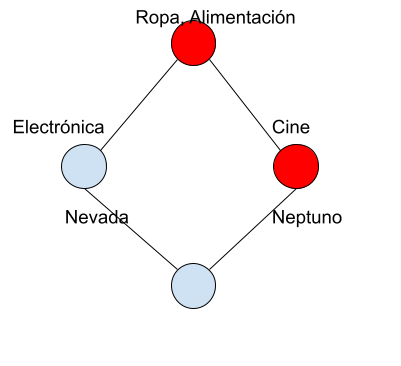
\includegraphics[scale=0.5]{images/addintent(1).png}
\caption{Retículo del contexto \ref{tab:comcercialesal} antes de añadir el objeto $\{g\}=\{SE\}$.}
  \label{fig:norris}

\end{figure}
Con esta información se va añadiendo el objeto $g$ a todos los conceptos que están por encima suya, y se añaden los atributos $\{g\}'$ a todos los conceptos que están por debajo suya, empezando por el generador.

En el peor de los casos el algoritmo tiene una complejidad de $O(|\G|^3 |\M| |L|)$ \cite{norris_algorithm_1978}.

\section{Propiedades}

A modo de resumen de la sección, presentamos una tabla comparativa (tabla \ref{tab:comparativa}) con las características más importantes de cada algoritmo que nos ayudará a entender mejor su desempeño en diferentes tipos de escenarios. Esta tabla es una versión adaptada de la que se puede encontrar en \cite{comparingperformance}, de la que hemos eliminado algunas propiedades poco útiles y a la que hemos añadido otras nuevas \footnote{las propiedades p2,p3,p4,p6,p7 no se encontraban en la tabla del artículo.}.

\begin{table}[H]
\centering
\begin{tabular}{|l|l|l|l|l|l|l|l|l|}
\hline
Algoritmo                         & \textbf{p1} & \textbf{p2} & \textbf{p3} & \textbf{p4} & \textbf{p5} & \textbf{p6} & \textbf{p7} & \textbf{p8} \\ \hline
\textbf{Next Closure (Ganter)}   &             & x           & x           & x           &             & x           &             &             \\ \hline
\textbf{Lindig}                   &             & x           &             & x           & x           &             & x           & x           \\ \hline
\textbf{InClose}                  &             & x           & x           & x           &             & x           &             & x           \\ \hline
\textbf{Inherit-Concepts (Berry)} &             & x           &             &             & x           &             &             &             \\ \hline
\textbf{Bordat}                   &             & x           &             &             &             &             & x           &             \\ \hline
\textbf{Norris}                   & x           &             &             &             & x           &             &             & x           \\ \hline
\textbf{Godin}                    & x           &             &             &             & x           &             &             & x           \\ \hline
\textbf{AddIntent}                & x           &             &             &             & x           &             & x           & x           \\ \hline
\end{tabular}
\caption{Tabla comparativa de todos los algoritmos: 
p1 - incremental;
p2 - por lotes;
p3 - utiliza el orden léxico;
p4 - en cada paso selecciona un concepto actual;
p5 - utiliza  alguna estructura auxiliar;
p6 - emplea un test de canonicidad para evitar repetir cálculos;
p7 - calcula vecinos de los conceptos;
p8 - calcula las intersecciones de las intensiones que no son objetos y las intensiones de los objetos;}
\label{tab:comparativa}
\end{table}

\part{Experimentación}

\chapter{Espacios de búsqueda}
   \label{chap:5}
Cuando se trabaja con cualquier algoritmo, el comportamiento de este va a estar determinado en gran medida por el conjunto de datos que reciba como entrada.  Para ver cómo se producen estos comportamientos, en este capítulo presentaremos unos conjuntos de datos sobre los que serán probados todos los algoritmos que hemos explicado en el capítulo anterior. 

Usualmente, los conjuntos de datos sobre los que se prueban los algoritmos son artificiales, lo cual se debe a varias razones. La principal es que los datos más interesantes del mundo real suelen tener un alto valor comercial y las empresas los mantienen confidenciales. Y por otro lado, muchas veces queremos ver el comportamiento de los algoritmos sobre conjuntos de datos con ciertas características, y estos son difíciles de encontrar presentes en el mundo real. Para ello, los conjuntos de datos generados aleatoriamente permiten explorar fácilmente el comportamiento de escalado de los algoritmos.

Pero el hecho de solo probarlos en conjuntos de datos artificiales puede resultar contraproducente, ya que podemos provocar un estudio de los algoritmos que poco tenga que ver con su desempeño real. Así finalmente nos hemos decidido por utilizar ambos tipos de conjuntos de datos.

Por último, es necesario destacar que nos hemos preocupado de almacenar y dejar disponibles públicamente todos los conjuntos de datos utilizados para esta experimentación para su uso posterior por parte de otros investigadores interesados en la materia. Se encuentran en el repositorio de GitHub creado para el \href{https://github.com/miguecl97/TFG-AlgoritmosFCA/tree/master/code/datasets}{trabajo}\footnote{https://github.com/miguecl97/TFG-AlgoritmosFCA/tree/master/code/datasets}.

Antes de presentarlos es interesante saber en qué características nos hemos fijado para seleccionar unos u otros.


\section{Métricas para los conjuntos de datos.}

Recordamos que, tal y como vimos en capítulos anteriores, los contextos vienen representados por lo que se denominan ``tablas cruzadas'', que no dejan de ser tablas cuya primera fila contiene los atributos y cuya primera columna contiene los objetos, con una $X$ en la casilla si el atributo y el objeto correspondientes están relacionados por $\I$. Por tanto lo que todos los conjuntos tienen en común es su estructura, una primera columna que comprenderán los objetos a estudio, y una primera fila que engloba los atributos del contexto. El factor diferencial y lo que los hace distintos entre ellos es la relación entre el conjunto de objetos y el conjunto de atributos. Esta relación, que los contextos la denotábamos por el símbolo $\I$, dará lugar a 3 métricas para poder comparar los distintos conjuntos.

La primera de ellas será el número de objetos, que determina el número de instancias que posee el conjunto de datos. A más objetos, más muestras tendrá nuestro conjunto de datos y más grande será en sentido ``vertical''. Si nos fijamos, en la mayoría de nuestros algoritmos la eficiencia teórica viene determinada de manera asintótica por $|\G|$.

En segundo lugar, el número de atributos $|\M|$ determinará también en parte la eficiencia del algoritmo. A mayor número de atributos más posibles relaciones pueden existir y por tanto más conceptos pueden existir. Pero la relación viene determinada por la cantidad de atributos que posea cada objeto, de donde obtenemos la tercera métrica.

Antes de conocer la tercera métrica, es interesante discutir una propiedad que posee la Teoría del Análisis Formal de Conceptos. Y es que la dualidad entre el conjunto de objetos $\G$ y el conjunto de atributos $\M$ nos permite intercambiarlos en sus papeles y poder aplicar todo lo visto en la primera parte del documento tomando un conjunto por el otro. Esto se traduce en que siempre que tengamos un conjunto de datos podríamos utilizar los atributos como objetos y viceversa, según nos convenga. Por ser más claros y precisos, en lo que en adelante sigue nunca alteraremos el orden entre los conjuntos y los mantendremos el conjunto de objetos como las filas del dataset y el conjunto de atributos como las columnas.

La tercera métrica que vamos a utilizar es el número medio de atributos que están relacionados con cada objeto. Denotaremos \footnote{Siguiendo la notación en artículos previos sobre la materia.} por $|g'|$  al número de atributos que poseen los objetos de $\G$, por tanto lo podemos definir como : $|g'|=\frac{\sum_{g \in \G}|\{g\}' |}{|\G|}$. Para los conjuntos de datos artificiales este número será el mismo para todos los objetos del conjunto. Sin embargo para los conjuntos de datos reales, tomaremos la media de todos los $|\{g\}'|$ con $g\in \G$. Por lo general, a mayor cantidad de atributos por cada objeto, mayor número de conceptos obtendremos en nuestro retículo (salvo casos triviales).

Si nos remontamos al ejemplo (\ref{monuments}) de los monumentos de Granada cuya tabla cruzada (\ref{tab:monumentos}) puede ser utilizada como un conjunto de datos: tendríamos que hay $|\G|=6$ objetos, $|\M|=4$ atributos y $|g'|=\frac{3+3+2+2+2+1}{6}=2,1$ número medio de atributos por objeto.

\section{Conjuntos de datos seleccionados.}

Para mejorar la estimación asintótica de la complejidad de los algoritmos, hemos construido contextos con conjuntos de datos artificiales con una complejidad creciente en cuanto a las $2$ de las $3$ métricas indicadas. Hemos decidido crear conjuntos de datos fijando en $100$ el número de atributos $|\M|$ (ya que es el que se usa en estudios previos de la materia \cite{comparingperformance}), y variando el número de objetos $|\G|$, y el número de atributos por objeto $|g'|$. La manera de generar los atributos que posee cada objeto se realiza de forma aleatoria generando $|g'|$ números entre $1$ y $|\M|$  siguiendo una distribución uniforme. Este hecho provocará que las diferencias entre las ejecuciones de un mismo algoritmo con dos conjuntos de datos con los mismos parámetros sean mínimas y obtengamos conjuntos de datos comparables conforme vayan escalando. El hecho de distribuir los atributos siguiendo una distribución uniforme se debe a que es una técnica estándar que se ha seguido en los trabajos anteriores en la materia, por lo que también nos es útil para comparar los resultados que obtengamos con los anteriores.  En la figura \ref{fig:distrartg40G100} se puede observar al distribución que siguen los atributos para un conjunto de datos con $|\M|=100$, $|g'|=40$ y $|\G|=100$.


\begin{figure}[H]
  \centering
  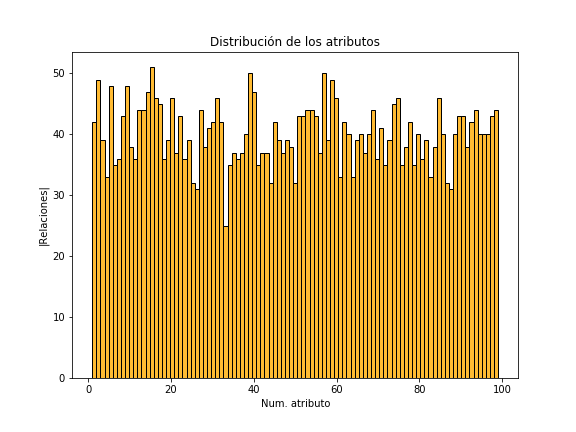
\includegraphics[scale=0.6]{images/distribution-artificialg40G100.png}
 
\caption{Histograma con el número de objetos con los que cada atributo está relacionado para el conjunto de datos artificial con $|\M|=100$, $|g'|=40$ y $|\G|=100$.}
 \label{fig:distrartg40G100}
\end{figure}

Los conjuntos de datos se encuentran disponibles en \href{https://github.com/miguecl97/TFG-AlgoritmosFCA/tree/master/code/datasets}{https://github.com/miguecl97/\linebreak TFG-AlgoritmosFCA/tree/master/code/datasets} y están clasificados para los experimentos de la siguiente manera:

Parámetros para los conjuntos de datos artificiales (cada configuración es un conjunto de datos):
\begin{itemize}
    \item \textbf{$|\M|=100$} , \textbf{$|g'|=10$}, \textbf{$|\G|=\{20,40,60,80,100\}$}.
    \item \textbf{$|\M|=100$} , \textbf{$|g'|=20$}, \textbf{$|\G|=\{20,40,60,80,100\}$}.
    \item \textbf{$|\M|=100$} , \textbf{$|g'|=30$}, \textbf{$|\G|=\{20,40,60,80,100\}$}.
    \item \textbf{$|\M|=100$} , \textbf{$|g'|=40$}, \textbf{$|\G|=\{20,40,60,80,100\}$}.
\end{itemize}

Para el primer caso, cuando $|g'|=10$, se obtienen muy pocos conceptos para cada contexto,y el tiempo de ejecución es mínimo, por lo que crearemos conjuntos de datos de mayor tamaño para comprobar sus límites:
\begin{itemize}
    \item \textbf{$|\M|=100$} , \textbf{$|g'|=10$}, \textbf{$|\G|=\{150,200,250,300,350,400,450,500\}$}.
\end{itemize}


Lo que hace un total de $28$ datasets con conjuntos de datos artificiales. Para comprobar que la generación aleatoria de la relación entre atributos y objetos no altera gravemente la forma del dataset (factor que desencadenaría en tiempos de ejecución muy diferentes para dos dataset con la misma configuración), se han generado por cada configuración $10$ datasets diferentes sobre los que se ejecutarán los algoritmos. En consecuencia se han producido $280$ ficheros $"$.csv$"$ con conjuntos de datos aleatorios para la experimentación. Los ficheros artificiales se encuentran en la carpeta \textit{datasets/M100}, y dentro de ella se dividen en $4$ subcarpetas según el valor de \textit{|g'|}. Dentro de ella los ficheros se llaman \textit{G(númeroobjetos)dataset(i).csv}, donde i indica el número de dataset que tiene esa forma. Por ejemplo, los conjuntos de datos con \textbf{$|\M|=100$}, \textbf{$|g'|=10$} y \textbf{$|\G|=\{20\}$} se pueden encontrar en la carpeta \textit{datasets/M100/g'10/} con el nombre \textit{G$20$dataset(i).csv}, con $i \in \{1,2,...,10\}$ para almacenar los $10$ conjuntos diferentes con los mismo parámetros.

Por otro lado, los conjuntos de datos reales se han obtenido realizando una binarización \cite{binarization} (o escalado) de los atributos no binarios para los conjuntos de datos disponibles en el repositorio de aprendizaje automático de la UCI \footnote{Universidad de California, Irvine} \cite{uci}. Los escogidos  han sido:

\begin{itemize}
    \item $"\textbf{Breast Cancer}".$ Contiene información recopilada por el doctor Wolberg \cite{breast} durante sus casos clínicos en relación con el cáncer de mama. Inicialmente este conjunto tiene $699$ objetos y $10$ atributos. Tras preprocesarlo y binarizar los atributos se obtienen finalmente $99$ atributos. Posteriormente para nuestro estudio recogimos una muestra de $500$ objetos. El número medio de atributos por objeto es $10$. El dataset original se encuentra disponible en \href{https://archive.ics.uci.edu/ml/machine-learning-databases/breast-cancer-wisconsin/}{https://archive.ics.uci.edu/\linebreak ml/machine-learning-databases/breast-cancer-wisconsin/} y el fichero csv que queda tras preprocesarlo se encuentra disponible en la carpeta \href{https://github.com/miguecl97/TFG-AlgoritmosFCA/tree/master/code/datasets/real-datasets/breastcancer.csv}{datasets/real-datasets/breastcancer.csv} \footnote{https://github.com/miguecl97/TFG-AlgoritmosFCA/tree/master/code/datasets/real\-datasets/breastcancer.csv} del repositorio de GitHub del trabajo.
    \item $"\textbf{Sponges}".$ Contiene información relativa a un estudio realizado sobre esponjas marinas que se encuentran en la costa del mediterráneo, con atributos como el color, el tipo de espora, el número de papilas, su forma, etc. Originalmente este conjunto de datos posee $76$ objetos y $45$ atributos. Para adaptarlo a nuestro experimento se ha realizado una binarización y eliminación de algunos atributos para obtener finalmente un fichero con $76$ objetos y $100$ atributos. El número medio de atributos por objeto es $29$. El dataset original se encuentra disponible en \href{https://archive.ics.uci.edu/ml/datasets/sponge}{https://archive.ics.uci.edu/ml/datasets/sponge} y el fichero csv tras haberlo preprocesado está en \href{https://github.com/miguecl97/TFG-AlgoritmosFCA/blob/master/code/datasets/real-datasets/sponge.csv}{datasets/real-datasets/sponge.csv} \footnote{https://github.com/miguecl97/TFG-AlgoritmosFCA/blob/master/code/datasets/real-datasets/sponge.csv} del repositorio de GitHub del trabajo.
\end{itemize}

En resumen, para los conjuntos de datos reales:
\begin{itemize}
    \item Breast-cancer.csv: \textbf{$|\M|=99$} , \textbf{$|g'|=10$}, \textbf{$|\G|=500$}.
    \item Sponges.csv: \textbf{$|\M|=100$} , \textbf{$|g'|=29$}, \textbf{$|\G|=76$}.
\end{itemize}

\chapter{Diseño del software}
   \label{chap:6}
En este capítulo explicaremos las pautas seguidas para implementar todo lo expuesto en las secciones previas. Comenzaremos explicando cómo hemos generado los conjuntos de datos y seguidamente los pasos seguidos para la implementación de los algoritmos. Todo el código relativo a esta implementación se encuentra disponible de manera pública en el repositorio de \textit{GitHub} utilizado para el trabajo \url{https://github.com/miguecl97/TFG-AlgoritmosFCA/tree/master/code}.

\section{Implementación de los algoritmos}

El lenguaje de programación elegido para la implementación del proyecto ha sido $C$++, ya que se trata de un lenguaje que conocemos bastante bien como producto de los años de estudio en el grado, se pueden reutilizar las funciones en el código, es fácilmente paralelizable en vista a un trabajo futuro, y la principal ventaja es que disponemos de librerías muy útiles como la \textit{Standard Template Library (STL)} que proporcionan herramientas como la clase \textit{'vector'} con una serie de funciones ya implementadas que nos han resultado de gran utilidad para el problema que abordamos. Aparte en artículos  anteriores sobre la materia \cite{comparingperformance} también ha sido el lenguaje utilizado para la implementación por lo que podemos establecer una comparación más cercana con el trabajo que ya existía.

El código se distribuye en varios ficheros, con funciones que ayudan a la ejecución de la experimentación y donde principalmente destacan las clases \textit{Lattice} y \textit{Context}. En el fichero \textit{main.cpp} se realiza la llamada a los algoritmos para realizar la experimentación del problema. En los ficheros \textit{batchalgorithms.cpp} e \textit{incrementalalgorithms.cpp} se encuentran varias funciones cada una correspondiente con el pseudocódigo del algoritmo implementado. Se ha optado por agrupar todos los algoritmos en los mismos ficheros para aumentar la consistencia del proyecto y reducir el número de clases empleadas. Por último el fichero \textit{utilities.cpp} contiene varias funciones auxiliares que resuelven problemas muy específicos que han ido surgiendo a lo largo del proyecto.

\textbf{Conceptos formales}

La principal estructura con la que se trabaja en todo el programa es la de concepto formal, decidimos implementarla como un par de vectores de números. Dichos números corresponden al objeto o atributo que ocupa esa posición en los vectores de atributos u objetos.

\begin{minted}[frame=lines]{c++}
    typedef pair<vector<int>, vector<int>> formalConcept; 
\end{minted}

\textbf{Clase Contexto}

Esta clase implementa lo que es un contexto formal $(\G,\M,\I)$ mediante un conjunto de datos (tabla) cuya primera columna corresponde a los objetos del contexto, mientras que la primera fila contiene el nombre de los atributos del mismo. El resto de casillas construyen la tabla cruzada que indica la relación $\I$ entre objetos y atributos, apareciendo un '$1$' en la casilla $(i,j)$ si el objeto número $i$ tiene el atributo número $j$. 

Esto lo implementamos en nuestro código definiendo los siguientes atributos para la clase Contexto:

\begin{minted}[frame=lines]{c++}
    size_t nObj, nProp; 
    vector<string> attributes; 
    vector<string> objects; 
    vector<vector<bool>> table; 
\end{minted}

Además de eso implementamos una serie de funciones que nos permiten consultar estos atributos desde fuera de la clase. También en esta clase se implementan herramientas importantes para los algoritmos como los operadores de derivación para objetos y atributos mediante las funciones:  

\begin{minted}[frame=lines]{c++}
        void objectPrime(vector<int> &objset, vector<int> &objPrime);
        void attributePrime(vector<int> &attrset, vector<int> &attributePrime);
\end{minted}


\textbf{Clase Retículo}

En la clase Retículo implementamos la estructura de retículo de conceptos mediante un vector de nodos, donde cada nodo contendrá la información relativa a un concepto. Por ello los atributos de la clase Lattice son:
\begin{minted}[frame=lines]{c++}
    int count;
    bool was_inserted;
    int last_position_index;
    vector<Node> concepts; 
\end{minted}

Los nodos del retículo están definidos mediante la siguiente estructura. Contienen el concepto y información relativa a los vecinos del nodo tanto superiores como inferiores, así como el índice en el que se ha insertado en el retículo:

\begin{minted}[frame=lines]{c++}
struct Node{
    int index;
    formalConcept c;
    pair<vector<int>,vector<int>> lowerUpperNeighbors;
}
\end{minted}

Además contiene funciones para insertar, buscar y reemplazar elementos del retículo, así como imprimirlos por pantalla o en un archivo.

\section{Obtención de los conjuntos de datos}

Como se mencionó en la sección anterior los conjuntos de datos reales han sido obtenidos del repositorio de la Universidad de California para \textit{'machine-learning'} disponible en \href{https://archive.ics.uci.edu/ml/datasets.php}{su página web} \footnote{https://archive.ics.uci.edu/ml/datasets.php}. Una vez descargados encontramos un problema en ellos y es que la mayoría de sus variables son categóricas o numéricas, y para aplicar los algoritmos de FCA necesitamos que todas estas sean variables categóricas nominales con dos posibles valores, 'sí' o 'no'. Ya que es la forma en la que implementamos el contexto en al tabla cruzada.

Para realizar este preprocesamiento se ha utilizado el lenguaje de programación \textit{PYTHON} (Python Software Foundation, \url{https://www.python.org/}) junto con la librería \textit{PANDAS} \cite{pandas}. Los conjuntos de datos reales son los disponibles ambos en la carpeta \textit{'datasets'} del repositorio que hemos utilizado para el trabajo. Y los scripts de python utilizados para su obtención y preprocesamiento están en la carpeta \textit{'utils'}.

Por otro lado, para los contextos artificiales, hemos implementado una función en el proyecto de $C++$ la cual construye un contexto formal con un número de objetos, atributos, y número de atributos que va a tener cada objeto como datos de entrada. Utilizando la clase \textit{uniform\_int\_distribution} generamos un número aleatorio en el intervalo $[1,|\M|]$ siguiendo una distribución uniforme. Repetimos dicho proceso $|g'|$ veces por fila y obtenemos el conjunto de datos deseado.

\begin{minted}[frame=lines]{c++}
Context generate(int nObj, int nProp, int nGPrime, int filenumber){
    vector<vector<bool>> mat(nObj, vector<bool>(nProp, false));
    const int range_from  = 1;
    const int range_to    = nProp;
    std::random_device                  rand_dev;
    std::mt19937                        generator(rand_dev());
    std::uniform_int_distribution<int>  distr(range_from, range_to);

    for(auto &row : mat){
        for(int i=0; i<nGPrime;i++){
            int random =distr(generator);
            while(row[random]==1){
                random = distr(generator);
            }
            row[random]=1;
        }
    }
    
    //...Se omite el proceso de volcar el contexto en un .csv..
    
    return Context(mat);
}
\end{minted}

\section{Librerías auxiliares}

Estas son las librerías más destacables que hemos necesitado a la hora de realizar el trabajo:

\begin{itemize}
    \item Para generar los atributos que posee cada objeto y que esta generación aleatoria siga una distribución uniforme, hemos utilizado la clase \href{https://en.cppreference.com/w/cpp/numeric/random/uniform_int_distribution}{uniform-int-distribution} \footnote{https://en.cppreference.com/w/cpp/numeric/random/uniform-int-distribution} de la librería \href{https://www.cplusplus.com/reference/random}{<random>} \footnote{https://www.cplusplus.com/reference/random} con la que podemos obtener valores aleatorios dentro de un intervalo $[a,b]$ y uniformemente distribuidos.
    \item Para la medición del tiempo de ejecución hemos utilizado la librería \href{https://en.cppreference.com/w/cpp/header/chrono}{<chrono>} \footnote{https://en.cppreference.com/w/cpp/header/chrono} de la STL. Tomando tiempos al inicio y al final de cada algoritmo obtenemos el tiempo de ejecución que tarda en obtener el retículo de conceptos, con una precisión de milisegundos.
    \item La librería \href{https://pandas.pydata.org/docs/}{\textit{pandas}} \footnote{https://pandas.pydata.org/docs/} de \textit{PYTHON} ha sido necesaria pra el preprocesamiento de los conjuntos de datos reales.
    \item Por último, la librería \href{https://concepts.readthedocs.io/en/stable/}{\textit{concepts}} \footnote{https://concepts.readthedocs.io/en/stable}. Otra librería de \textit{PYTHON} que nos permite trabajar con el FCA, la hemos utilizado para comprobar que los resultados de los algoritmos eran correctos y generar la representación gráfica de algunos retículos.
\end{itemize}

\section{Validación del software}

Las pruebas de unidad nos permiten comprobar el correcto funcionamiento de nuestros algoritmos. Dentro de estas se distinguen dos tipos según si nos fijamos en la estructura interna del  algoritmo ($"$pruebas de caja blanca$"$) o tratándolos como una caja negra para comprobar que con cierta entrada se produce cierta salida ($"$pruebas de caja negra$"$).

Durante el desarrollo del software todas las funciones programadas han sido probadas mediante pequeños tests manuales para comprobar que en los casos límite funcionan correctamente.

A modo de pruebas de caja negra, las más importantes para asegurarnos de que nuestro software está realizando su función correctamente, hemos ido recopilando pequeños conjuntos de datos que los autores proporcionan en la literatura, con la salida que estos mismos especifican. Y así hemos comprobado que tomando los mismos conjuntos de datos se obtienen exactamente los mismos conceptos que los autores indican en la literatura. A su vez, para los conjuntos de datos creados para ilustrar este documento, sus retículos los hemos obtenido utilizando la librería \textit{concepts} de python, y posteriormente hemos comprobado que nuestros algoritmos nos proporcionan la misma salida. Los test de caja negra se encuentran disponibles en \href{https://github.com/miguecl97/TFG-AlgoritmosFCA/tree/master/code/blackBoxTests}{https://github.com/miguecl97/TFG-AlgoritmosFCA/tree/master/code/blackBoxTe\linebreak sts}.

Otra de las evidencias de que nuestro software es correcto es que en todas las ejecuciones de nuestra experimentación, todos los algoritmos proporcionan el mismo número de conceptos ante el mismo conjunto de datos de entrada .

\chapter{Resultados del experimento}
   \label{chap:7}
Estamos ya en condiciones de comenzar la experimentación de los algoritmos con los conjuntos de datos escogidos. En primer lugar, comentaremos qué es lo que se desea conseguir con estos experimentos, seguidamente seleccionaremos las métricas que nos explicarán el desempeño de los algoritmos, en tercer lugar indicaremos los recursos de los que dispone el sistema utilizado, y por último comentaremos los resultados obtenido en conjunto.

\section{Objetivos del experimento}

En un escenario ideal, la meta principal de esta experimentación es comprobar cómo se comportan los algoritmos según el conjunto de datos que se utiliza como entrada, y además verificar la eficiencia en tiempo a nivel asintótico que los autores proporcionan en cada uno de los artículos. Hay varios artículos que han tratado de replicar este procedimiento en la literatura \cite{comparingperformance}, \cite{comparingcorta} o \cite{comparing3}. Quizás el más relevante de todos sea el primero de ellos, realizado en 2002 por Sergei O. Kuznetsov. Nuestro trabajo estará enfocado en comprobar la experimentación realizada por el autor y en el mejor de los casos obtener mejoras en la eficiencia provocadas por la mayor capacidad computacional que poseemos en ventaja a la que había al principio del milenio. Además nuestra experimentación incluye nuevos algoritmos como el de Berry o el InClose.

Por ello nuestro principal objetivo será qué algoritmos funcionan mejor según el conjunto de datos que reciban como entrada. Analizaremos la eficiencia en cuanto a tiempo de ejecución de los algoritmos, ya que en vistas a los primeros experimentos que hicimos los algoritmos no ocupaban apenas los recursos de almacenamiento del sistema. Aún en los datasets de mayor densidad había algoritmos que tardaban más de $20$ minutos en ejecutarse y apenas ocupaban menos de $1GB$ de memoria RAM de almacenamiento.

Aparte de los tiempos de ejecución que se han analizado, los retículos minados por cada algoritmo en cada iteración se encuentran disponibles en la carpeta \textit{results} del \href{https://github.com/miguecl97/TFG-AlgoritmosFCA/tree/master/code}{repositorio de GitHub} \footnote{https://github.com/miguecl97/TFG-AlgoritmosFCA/tree/master/code} del trabajo. Los retículos se muestran en ficheros de texto planos donde las primeras líneas de cada algoritmo incluye la medición de los tiempos de ejecución del algoritmo y seguidamente se muestra la lista de conceptos correspondiente al retículo. Siguen la misma estructura de almacenamiento en carpetas que los conjuntos de datos de entrada.


\section{Entorno de ejecución}

Los experimentos han sido ejecutados en un Intel\textregistered $ \ $ Core\texttrademark $ \ $ i5-8265U CPU $@$ 1.60GHz × 8 , con 7,6 Gigabytes de RAM bajo el sistema operativo Ubuntu 19.10. Los ficheros de código han sido compilados utilizando el compilador \textit{g++} con la opción de optimización $-O2$ por ser la que mayor mejora de rendimiento en cuanto a tiempo de ejecución nos ha aportado tras realizar varias ejecuciones con diferentes conjuntos de datos de prueba. 

\section{Resultados}

A continuación presentaremos los resultados obtenidos midiendo el tiempo de ejecución de los algoritmos ante conjuntos de datos con diferentes parámetros. Utilizaremos gráficas para sintetizar y presentar toda la información obtenida. Las ejecuciones detalladas se pueden consultar en el apéndice \ref{apendiceb} que se encuentra al final del documento.

\subsection{ Conjuntos de datos artificiales}

\begin{itemize}


\item \textbf{$|\M|=100$} \textbf{$|g'|=10$} \textbf{$|\G|=\{20,40,60,80,100\}$}.\\

En este primer experimento (gráfica \ref{fig:m100g10g20100}) observamos que ante conjuntos con pocos atributos por objeto, la mayoría de algoritmos funcionan de manera similar, destacando de forma negativa el algoritmo AddIntent que, cuando el conjunto de objetos alcanza un tamaño de 100 objetos, empeora considerablemente su desempeño con respecto al resto de algoritmos. Pare hacer justicia, hemos de indicar que este comportamiento puede deberse a que la implementación del método para obtener los padres de un concepto que hemos realizado no sea la más eficiente de todas, ya que el autor no proporciona ninguna indicación para realizar dicho proceso. Por este motivo, y teniendo en cuenta que este rendimiento no mejora cuando el conjunto de datos escala, el algoritmo AddIntent será eliminado del resto de gráficas para obtener una comparación más visual.

\begin{figure}[H]
  \centering
  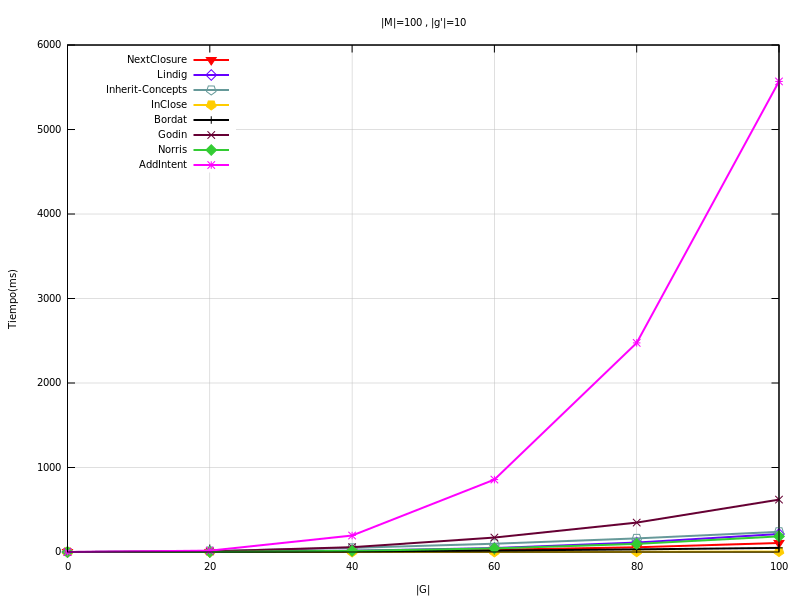
\includegraphics[scale=0.5]{images/M100g10G20100.png}
\caption{Gráfica comparativa con los tiempos de ejecución de cada algoritmo sobre conjuntos de datos con $|\M|=100$ y $|g'|=10$.}
  \label{fig:m100g10g20100}
\end{figure}

En la gráfica \ref{fig:m100g10g20100nadd} se ha eliminado el algoritmo AddIntent. Vemos que para este tipo de conjuntos de datos el algoritmo de Godin tampoco tiene un buen rendimiento mientras que el algoritmo InClose es el más rápido, obteniendo tiempos realmente bajos y estables aunque aumente el número de objetos. En el siguiente experimento aumentaremos el número de objetos para ver cómo evoluciona su comportamiento.

\begin{figure}[H]
  \centering
  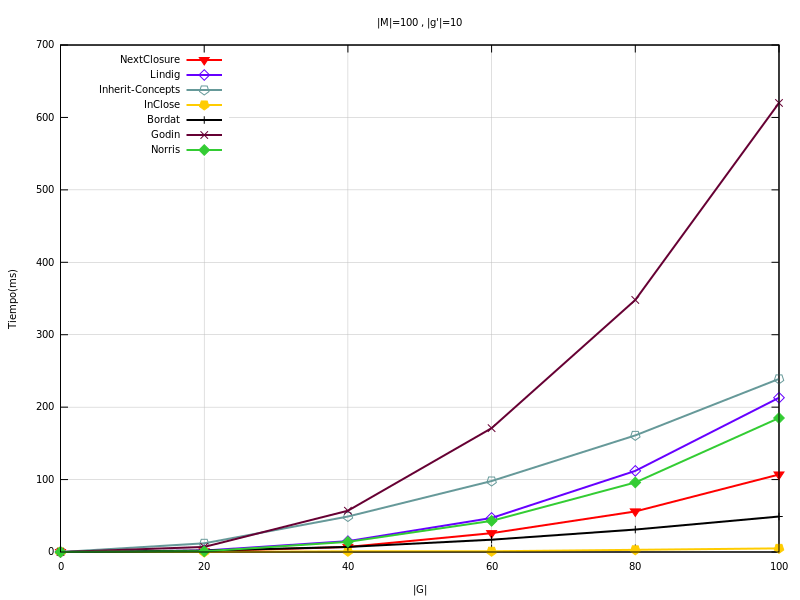
\includegraphics[scale=0.5]{images/M100g10G20100notadd.png}
\caption{Gráfica comparativa con los tiempos de ejecución de cada algoritmo sobre conjuntos de datos con $|\M|=100$ y $|g'|=10$ sin AddIntent.}
  \label{fig:m100g10g20100nadd}
\end{figure}

\item \textbf{$|\M|=100$} \textbf{$|g'|=10$} \textbf{$|\G|=\{100,150,200,250,300,350,400,450,500\}$}.\\

Bajo las mismas condiciones que el experimento anterior, manteniendo la baja densidad del dataset, cuando aumenta el tamaño del conjunto de datos las diferencias entre los algoritmos se van acentuando. Sin embargo los algoritmos InClose y Bordat se mantienen estables teniendo una eficiencia realmente buena cuando el conjunto de datos adopta un tamaño considerable. Este hecho lo podemos ver representado en la figura \ref{fig:m100g10g100500}.

\begin{figure}[H]
  \centering
  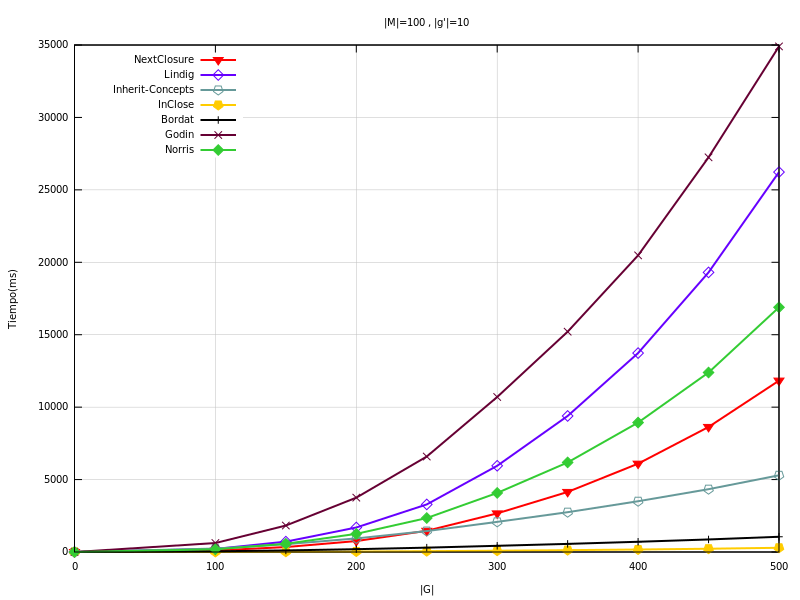
\includegraphics[scale=0.5]{images/M100g10G100500notadd.png}
\caption{Gráfica comparativa con los tiempos de ejecución de cada algoritmo sobre conjuntos de datos con $|\M|=100$ y $|g'|=10$.}
  \label{fig:m100g10g100500}
\end{figure}

\item \textbf{$|\M|=100$} \textbf{$|g'|=20$} \textbf{$|\G|=\{20,40,60,80,100\}$}.\\

Para este experimento aumentamos a 20 el número de atributos que posee cada objeto. Con este cambio apreciamos cómo los algoritmos empeoran su rendimiento respecto al experimento anterior, hecho debido a que aumenta la densidad y se minan más conceptos por cada dataset. Como se puede apreciar en la gráfica \ref{fig:m100g20g20100}, el algoritmo InClose sigue siendo el que mejor desempeño ofrece, pero por otro lado, el de Bordat ha empeorado su rendimiento, llegando a dar un peor tiempo de ejecución que el NextClosure. Otro hecho destacable es que el algoritmo de Lindig en el paso de 60 a 100 objetos pasa de ser el cuarto mejor algoritmo a emparejarse con el sexto en tiempos de ejecución.

\begin{figure}[H]
  \centering
  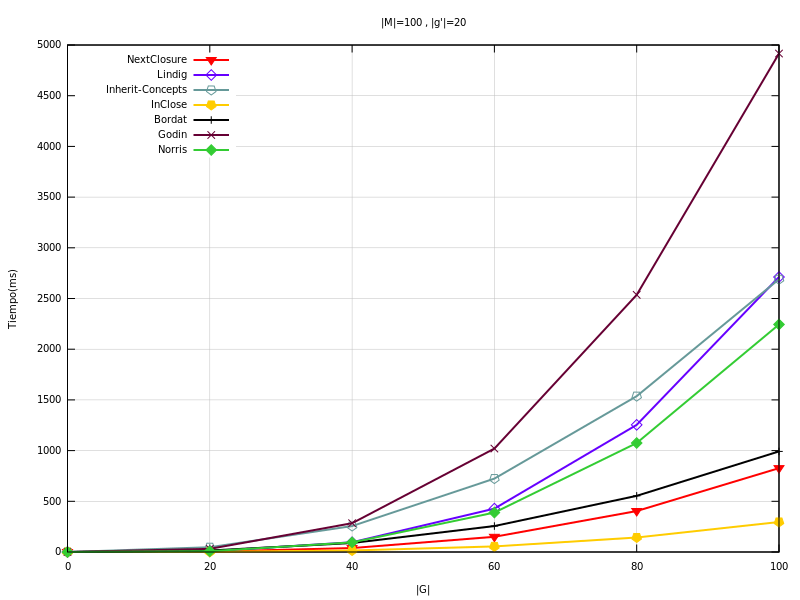
\includegraphics[scale=0.5]{images/M100g20G20100.png}
\caption{Gráfica comparativa con los tiempos de ejecución de cada algoritmo sobre conjuntos de datos con $|\M|=100$ y $|g'|=20$.}
  \label{fig:m100g20g20100}
\end{figure}


\item \textbf{$|\M|=100$} \textbf{$|g'|=30$} \textbf{$|\G|=\{20,40,60,80,100\}$}.\\

El siguiente caso a estudiar es cuando el número de atributos por objeto es de 30. Con este cambio el conjunto de datos aumenta considerablemente su densidad con respecto a los casos anteriores. Al aumentar su densidad se aprecian grandes cambios en los tiempos de ejecución. Como es el caso del algoritmo de Lindig, que al trabajar con un conjunto de datos de 100 objetos tiene una gran caída en su rendimiento. Por el contrario vemos que el algoritmo InClose deja de ser el que mejor rendimiento nos ofrece. En estos casos el algoritmo NextClosure se mantiene más estable en cuanto a términos de eficiencia en tiempo de ejecución. Este fenómeno puede deberse a que al aumentar el número de relaciones en la tabla, el método de poda del algoritmo InClose pierde utilidad, ya que aumentando el número de atributos se le impide podar antes la rama para pasar al siguiente concepto. Además los algoritmos de Bordat y de Norris intercambian posiciones al pasar de 80 a 100 objetos.

\begin{figure}[H]
  \centering
  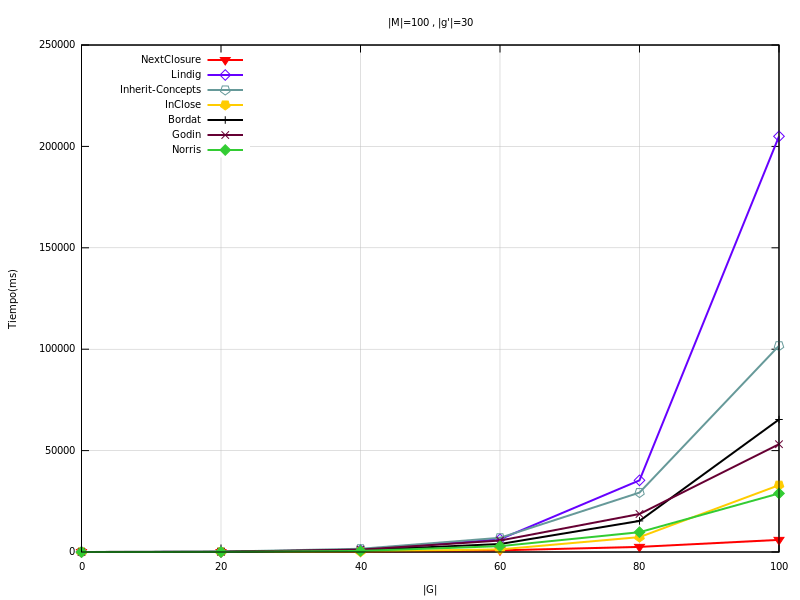
\includegraphics[scale=0.5]{images/M100g30G20100.png}
  \label{fig:m100g30g20100}
\caption{Gráfica comparativa con los tiempos de ejecución de cada algoritmo sobre conjuntos de datos con $|\M|=100$ y $|g'|=30$.}
\end{figure}

\item \textbf{$|\M|=100$} \textbf{$|g'|=40$} \textbf{$|\G|=\{10,20,30,40,50,60,70,80\}$}.

Para este último experimento volvemos a aumentar en 10 el número de atributos que posee cada objeto de la tabla, terminando en 40. Este valor para el parámetro $|g'|$ provoca que se generen un gran número de conceptos para cada contexto, lo que se traduce en un aumento considerable en los tiempos de ejecución y en los recursos del sistema. Este es el motivo por el que algunos algoritmos no se siguen ejecutando para valores grandes de $|\G|$.  El resultado de este experimento es que al llegar a la cifra de $|G|=60$ varios algoritmos comienzan a empeorar su desempeño de manera notable. El algoritmo de Lindig que anteriormente vimos que perdía bastante eficiencia, confirma este suceso, uniéndose a él los algoritmos de Inherit-Concepts y Bordat. No nos sorprende que el algoritmo Inherit-Concepts sea el segundo que peor rendimiento ofrece ya que las tablas $T$ y $D$ que utiliza para mantener información alcanzan un tamaño considerable, y esto provoca que su actualización sea costosa. Por otro lado el algoritmo NextClosure se confirma como el mejor candidato a la hora de ejecutar contextos con una densidad elevada. Cuando pasamos a $|\G|=80$, los algoritmos de Norris, InClose y Godin se disparan en el tiempo de ejecución, y el único que se mantiene estable es el de NextClosure. Este hecho es muy similar al que ocurrió en la experimentación realizada por Obiedkov \cite{comparingperformance}.

\begin{figure}[H]
  \centering
  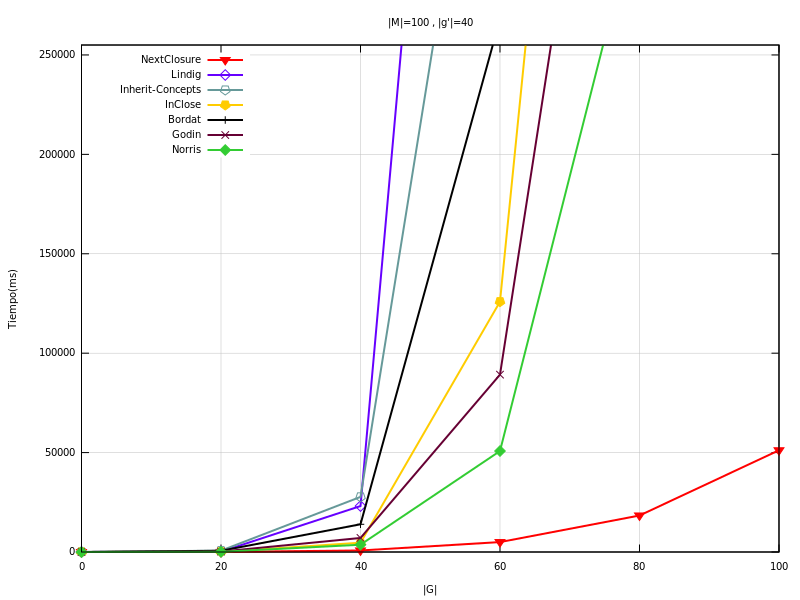
\includegraphics[scale=0.5]{images/M100g40G20100.png}
  \label{fig:m100g40g20100}
\caption{Gráfica de comparación de algoritmos con $|\M|=100$ y $|g'|=40$.}
\end{figure}


\textbf{Ventaja en tiempo de ejecución de los algoritmos incrementales}\\

Nos planteamos ahora que si utilizando la principal propiedad de los algoritmos incrementales podríamos obtener alguna ventaja para este último caso. Suponiendo que tengamos que añadir 20 nuevos objetos a nuestro retículo, vamos a simular que para nuestra aplicación en primer lugar construimos el retículo con los primeros 60 objetos que recibamos, y posteriormente queremos añadir 20 más, hasta llegar a 80. Para ello resumimos en una tabla el tiempo de ejecución que emplearía cada uno. En el caso del NextClosure, habría que construir primero el retículo con los primeros 60 objetos, y al añadir 20, deberíamos de volver a construir desde cero el retículo pero ahora con 80 objetos, por lo que habría que sumar ambos tiempos. Por el contrario, los incrementales van añadiendo esos 20 objetos al retículo ya construido por lo que simplemente tomamos el tiempo que tardan en construir el retículo de 80. Tal y como se observa en la tabla \ref{tab:increment}, sigue siendo más eficiente construir el retículo de nuevo por completo con el algoritmo NextClosure.

\begin{table}[H]
\resizebox{15.9cm}{!}{
\begin{tabular}{l|l|l|l|l|}
\hline
\multicolumn{1}{|l|}{$|g'|$} & $|\G|$                                        & NextClosure & Norris   & Godin    \\ \hline
\multicolumn{1}{|l|}{40}     & 60                                            & 4990        & 50786    & 89212,9  \\ \hline
\multicolumn{1}{|l|}{40}     & 80                                            & 18359,5     & 327035,3 & 542232,6 \\ \hline
                             & Tiempo(ms) en añadir 20 objetos (de 60 a 80): & 23349,5     & 327035,3 & 542232,6 \\ \cline{2-5} 
\end{tabular}
}
\caption{Tabla comparativa de tiempos de ejecución en ms para $|\M|=100$, que tardaría cada algoritmo en añadir 20 objetos al retículo.}
\label{tab:increment}
\end{table}

\end{itemize}

Para buscar un caso donde nos sea rentable la principal utilidad de los algoritmos incrementales nos debemos remontar a la figura \ref{fig:m100g10g20100nadd}. En este experimento recordamos que el algoritmo de Godin era el más lento. Pero el de Norris y el NextClosure tenían rendimientos similares, siendo el de NextClosure el más rápido a la hora de construir el retículo de 100 objetos por lotes. Veamos en la siguiente tabla \ref{tab:incremen10} lo que tardaría cada algoritmo en construir de manera incremental el retículo añadiendo en cada ocasión 20 objetos al contexto.

\begin{table}[H]
\resizebox{15.9cm}{!}{
\begin{tabular}{|l|l|l|l|l|l|}
\hline
$|g'|$ & $|\G|$             & NextClosure & Norris & NextClosure (incrementalmente) & Norris (incrementalmente) \\ \hline
10     & 20                 & 1           & 1,8    & 1                         & 1,8                  \\ \hline
10     & 40                 & 7,6         & 7,88   & 8,6                       & 7,88                 \\ \hline
10     & 60                 & 26,7        & 43,88  & 35,3                      & 43,88                \\ \hline
10     & 80                 & 56,2        & 95     & 91,5                      & 95                   \\ \hline
10     & 100                & 107,1       & 185,1  & 198,6                     & 185,1                \\ \hline
       & Tiempo total (ms): &             &        & 197,1                     & 185,1                \\ \hline
\end{tabular}
}
\caption{Tabla comparativa de tiempos de ejecución para una ejecución incremental con $|\M|=100$ y $|g'|=10$.}

\label{tab:incremen10}
\end{table}

En este caso vemos como el algoritmo de Norris nos ofrece cierta mejoría en cuanto a tiempo de ejecución a la hora de realizar esta tarea, aunque no sea muy apreciable. Esto deja claro el hecho de que es necesario mejorar y actualizar los algoritmos incrementales que existen en la literatura.

\subsection{Conjuntos de datos reales}
\begin{itemize}
\item \textbf{Breast-cancer.csv}

Para el conjunto de datos reales con información acerca del cáncer de mama los tiempos de ejecución (en milisegundos) por algoritmo que hemos obtenido han sido:

\begin{table}[H]
    \centering
    \resizebox{15.9cm}{!}{
    \begin{tabular}{|l|l|l|l|l|l|l|l|l|}
    \hline
        $|g'|$ & $|\G|$ & NextClosure & Lindig & Inherit-Concepts & InClose & Bordat & Godin & Norris \\ \hline
        10 & 500 & 8788,2 & 14262,6 & 3193 & 42,7 & 1400,8 & 17671,8 & 8153,3 \\ \hline
    \end{tabular}
    }
    \caption{Tabla de tiempos de ejecución en ms para el conjunto de datos de cáncer de pulmón.}
\end{table}

\begin{figure}[H]
  \centering
  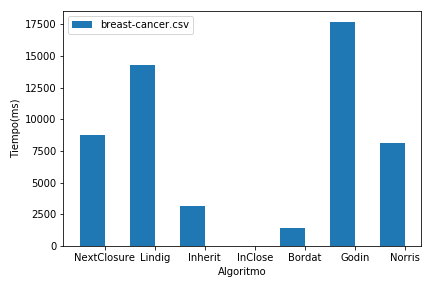
\includegraphics[scale=0.6]{images/total-breast.png}
  \label{fig:totalbreast}
\caption{Gráfica de tiempos de ejecución de cada algoritmo para el conjunto de datos real }
\end{figure}
Apreciamos que el algoritmo InClose es el más rápido con diferencia con respecto a sus competidores, seguido por el algoritmo de Bordat y el InheritConcepts. Cabe preguntarnos si este comportamiento se corresponde con el estudiado en nuestros conjuntos de datos artificiales, por ello, compararemos el tiempo de ejecución obtenido con el del dataset artificial con las características más parecidas $|\M|=100$, $|\G|=500$ y $|g'|=10$.
\begin{table}[H]
    \centering
    \resizebox{15.9cm}{!}{
    \begin{tabular}{|l|l|l|l|l|l|l|l|l|l|}
    \hline
        Dataset & $|g'|$ & $|\G|$ & NextClosure & Lindig & Inherit-Concepts & InClose & Bordat & Godin & Norris \\ \hline
        breas-cancer.csv & 10 & 500 & 8788,2 & 14262,6 & 3193 & 42,7 & 1400,8 & 17671,8 & 8153,3 \\ \hline
        artificial & 10 & 500 & 11830,5 & 26228,4 & 5295,1 & 291,6 & 1052,8 & 34903,9 & 16893,1 \\ \hline
    \end{tabular}
    }
    \caption{Tabla comparativa de tiempos de ejecución en ms para el conjunto de datos de cancer de pulmon y uno artificial.}
\end{table}

\begin{figure}[H]
  \centering
  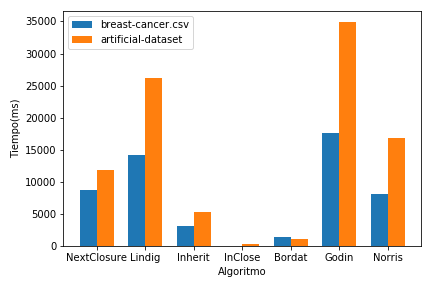
\includegraphics[scale=0.6]{images/comparative-breast.png}
\caption{Gráfica comparativa de tiempos de ejecución de cada algoritmo entre el conjunto de datos real y artificial del mismo tamaño. }
\label{fig:compbreast}
\end{figure}

En la figura \ref{fig:compbreast} podemos observar que el comportamiento es bastante parecido y, aunque se obtienen tiempos diferentes, los algoritmos siguen prácticamente el mismo orden. Esta diferencia de tiempos se debe en mayor medida a la distribución de los atributos para cada objeto. Ya que en nuestro dataset artificial se seguía una distribución uniforme y el conjunto breast-cancer.csv probablemente no la siga. En efecto, en la figura \ref{fig:disbreast} se puede ver la distribución que siguen los atributos del dataset, que está lejos de seguir una distribución uniforme. Mientras que en la figura \ref{fig:distrartg10G500} vemos la distribución que siguen los atributos para el conjunto de datos artificial sobre el que habíamos realizado el estudio. Estas diferencias probablemente son las que provocan los cambios de rendimiento en los algoritmos.

\begin{figure}[H]
  \centering
  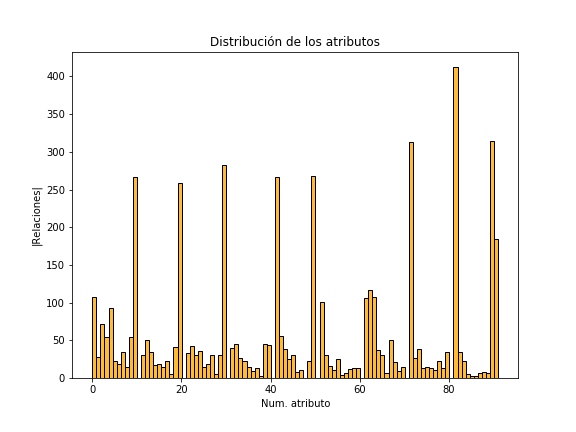
\includegraphics[scale=0.5]{images/distribution-breast.png}
 
\caption{Histograma con el número de objetos con los que cada atributo está relacionado para el conjunto de datos breastcancer.csv .}
 \label{fig:disbreast}
\end{figure}

\begin{figure}[H]
  \centering
  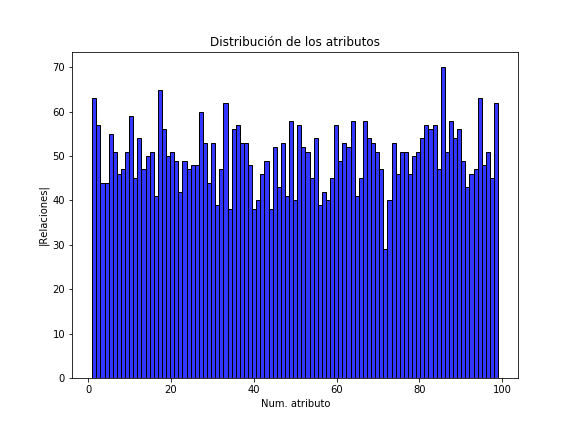
\includegraphics[scale=0.5]{images/distribution-artificialg10G500.png}
 
\caption{Histograma con el número de objetos con los que cada atributo está relacionado para el conjunto de datos artificial con $|\M|=100$, $|g'|=10$ y $|\G|=500$.}
 \label{fig:distrartg10G500}
\end{figure}

\clearpage

\item \textbf{Sponges.csv}

Para el conjunto de datos con información de un estudio de esponjas marinas de la costa mediterránea los tiempos de ejecución obtenidos han sido los siguientes:

\begin{table}[H]
    \centering
    \resizebox{15.9cm}{!}{
    \begin{tabular}{|l|l|l|l|l|l|l|l|l|}
    \hline
        $|g'|$ & $|\G|$ & NextClosure & Lindig & Inherit-Concepts & InClose & Bordat & Godin & Norris \\ \hline
        29 & 79 & 1328 & 3865,8 & 9590,1 & 309,4 & 7933,9 & 6651,4 & 3058,4 \\ \hline
    \end{tabular}
    }
    \caption{Tabla de tiempos de ejecución en ms para el conjunto de datos de esponjas y uno artificial.}
\end{table}

\begin{figure}[H]
  \centering
  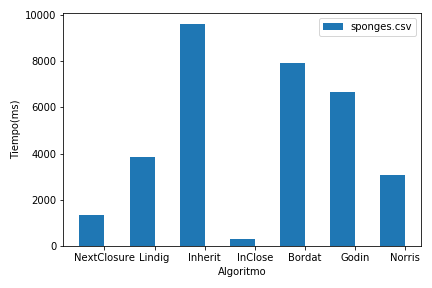
\includegraphics[scale=0.6]{images/total-sponges.png}
  
\caption{Gráfica de tiempos de ejecución de cada algoritmo para el conjunto de datos real }
\label{fig:totalsponges}
\end{figure}
 Tal y como se aprecia en la figura \ref{fig:totalsponges} el algorimo InClose vuelve a ser el más rápido, seguido del NextClosure. Veamos si se corresponde con las pruebas realizadas anterioremente:
\begin{table}[H]
    \centering
    \resizebox{15.9cm}{!}{
    \begin{tabular}{|l|l|l|l|l|l|l|l|l|l|}
    \hline
        Dataset & $|g'|$ & $|\G|$ & NextClosure & Lindig & Inherit-Concepts & InClose & Bordat & Godin & Norris \\ \hline
        sponge.csv & 29 & 76 & 1328 & 3865,8 & 9590,1 & 309,4 & 7933,9 & 6651,4 & 3058,4 \\ \hline
        artificial & 30 & 80 & 2522,9 & 35337,1 & 29299,8 & 7346,3 & 15327,3 & 18749,6 & 9769,1 \\ \hline
    \end{tabular}
    }
    \caption{Tabla comparativa de tiempos de ejecución en ms para el conjunto de datos de esponjas.}
\end{table}

Ahora el resultado obtenido es bastante diferente, para el conjunto de datos artificial con la misma forma que el real el algoritmo NextClosure era el más rápido y el InClose era bastante más lento. Por otro lado destaca la diferencia de ejecución del algoritmo de Lindig que para el conjunto de datos real es 7 veces más rápido.

\begin{figure}[H]
  \centering
  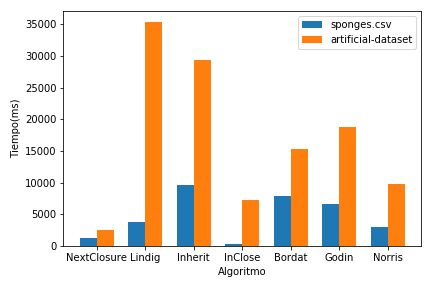
\includegraphics[scale=0.6]{images/comparative-sponges.png}
  
\caption{Gráfica comparativa de tiempos de ejecución de cada algoritmo entre el conjunto de datos real y artificial del mismo tamaño. }
\label{fig:compsponges}
\end{figure}
\end{itemize}

De nuevo estos cambios probablemente se deban a la diferencia en las distribuciones de los atributos entre los conjuntos de datos artificiales y real. Los conjuntos que hemos generado seguían una distribución uniforme (figura \ref{fig:distrartg30G80}) en el número de relaciones que tiene cada atributo y el conjunto de datos de esponjas se distribuye de la siguiente manera (figura \ref{fig:dissponges}):

\begin{figure}[H]
  \centering
  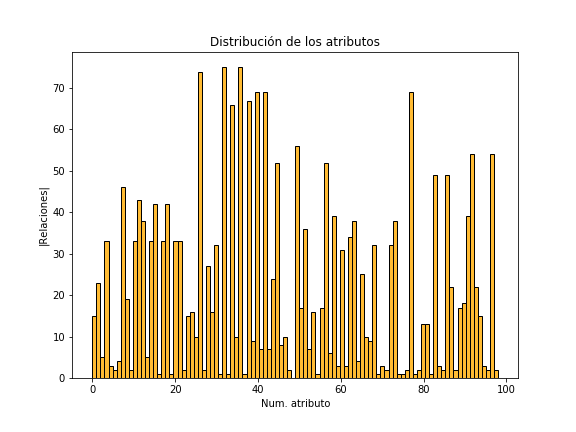
\includegraphics[scale=0.5]{images/distribution-sponges.png}
\caption{Histograma con el número de objetos con los que cada atributo está relacionado para el conjunto de datos sponges.csv. }
  \label{fig:dissponges}

\end{figure}

\begin{figure}[H]
  \centering
  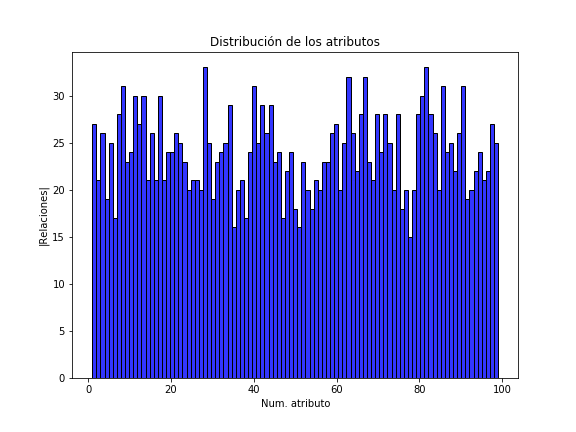
\includegraphics[scale=0.5]{images/distribution-artificialg30G80.png}
\caption{Histograma con el número de objetos con los que cada atributo está relacionado para el conjunto de datos artificial con $|\M|=100$, $|g'|=30$ y $|\G|=80$.}
 \label{fig:distrartg30G80}
\end{figure}

En ambos conjuntos de datos reales obtenemos diferencias con respecto a la experimentación que se ha hecho anteriormente con los datos artificiales. La explicación que encontramos a este comportamiento es la diferencia en la distribución de los atributos del contexto. En efecto, si creamos dos contextos con las mismas características, por ejemplo $|\M|=4$, $|g'|=2$ y $|\G|=3$, y en uno de ellos (tabla \ref{tab:uniforme}) distribuimos los atributos uniformemente, pero en el otro (tabla \ref{tab:nouniforme}) no los distribuimos uniformemente, obtenemos dos retículos de conceptos totalmente diferentes con conceptos diferentes en tamaño y en forma.

\begin{figure}[H]
\centering
\begin{minipage}{.4\textwidth}
  \centering
    \begin{table}[H]
    \begin{tabular}{|l|l|l|l|l|}
    \hline
       & a1 & a2 & a3 & a4 \\ \hline
    o1 & ~  & X  & X  & ~  \\ \hline
    o2 & X  & ~  & X  & ~  \\ \hline
    o3 & ~  & X  & ~  & X  \\ \hline
    \end{tabular}
    \caption{Ejemplo de un contexto uniforme.}
    \label{tab:uniforme}
    \end{table}
\end{minipage}%
\begin{minipage}{.6\textwidth}
  \centering
Retículo de conceptos del contexto de la tabla \ref{tab:uniforme}:\\
\begin{itemize}
    \item Concepto 1: (\{\}, \{a1, a2, a3, a4\}) 
    \item Concepto 2: (\{o1\}, \{a2, a3\}) 
    \item Concepto 3: (\{o2\}, \{a1, a3\}) 
    \item Concepto 4: (\{o3\}, \{a2, a4\}) 
    \item Concepto 5: (\{o1, o2\}, \{a3\}) 
    \item Concepto 6: (\{o1, o3\}, \{a2\}) 
    \item Concepto 7: (\{o1, o2, o3\}, \{\}) 
\end{itemize}
\end{minipage}
%\caption{Ejemplo de un contexto con $|\M|=4$, $|g'|=2$ y $|\G|=3$ , con una distribución que siguen los atributos que es uniforme junto con la lista de conceptos de su retículo. }
  %\label{fig:test1}
\end{figure}

\begin{figure}[H]
\centering
\begin{minipage}{.4\textwidth}
  \centering
    \begin{table}[H]
    \begin{tabular}{|l|l|l|l|l|}
    \hline
       & a1 & a2 & a3 & a4 \\ \hline
    o1 & X  & X  & ~  & ~ \\ \hline
    o2 & X  & ~  & ~  & ~  \\ \hline
    o3 & X  & ~  & X  & X  \\ \hline
    \end{tabular}
    \caption{Ejemplo de un contexto no uniforme.}
    \label{tab:nouniforme}
    \end{table}
\end{minipage}%
\begin{minipage}{.6\textwidth}
  \centering
Retículo de conceptos del contexto de la tabla \ref{tab:nouniforme}:
\begin{itemize}
    \item Concepto 1: (\{\}, \{a1, a2, a3, a4\}) 
    \item Concepto 2: (\{o1\}, \{a1, a2\}) 
    \item Concepto 3: (\{o3\}, \{a1, a3, a4\}) 
    \item Concepto 4: (\{o1, o2, o3\}, \{a1\}) 
\end{itemize}
\end{minipage}
%\caption{Ejemplo de un contexto con $|\M|=4$, $|g'|=2$ y $|\G|=3$ , con una distribución que siguen los atributos que no es uniforme junto con la lista de conceptos de su retículo. }
  %\label{fig:test1}
\end{figure}








\section{Discusión de los resultados de la experimentación}

Una vez concluida la experimentación, a modo de síntesis, en esta sección nos centraremos en los resultados del estudio y la información que hemos extraído de ellos. 

Para los conjuntos de datos artificiales, hemos podido apreciar cómo los algoritmos trabajan muy rápido ante conjuntos de datos con poca densidad, obteniendo tiempos de ejecución en general muy bajos con respecto a los conjuntos de datos con densidad elevada. Este fenómeno se debe en gran medida a que al aumentar el número de relaciones existentes en el contexto, el número de conceptos que posee también aumenta. En el mayor de los casos estudiados, para $|M|=100$, $|\G|=80$, $|g'|=40$ se minaron $370683$ conceptos por cada algoritmo. Este hecho hace que tengamos que ser muy cuidadosos a la hora de escoger el algoritmo a utilizar en este tipo de conjuntos de datos, teniendo como opciones válidas el NextClosure o el algoritmo de Norris, según si el conjunto de datos va a ser actualizado con frecuencia o no. Por otro lado, si nos encontramos ante un problema con un contexto de poca densidad la elección del algoritmo no penalizará tanto el rendimiento de la aplicación, aunque según nuestro estudio el algoritmo InClose, gracias a su mecanismo de poda, es el más rápido y el que mantiene una mayor estabilidad conforme aumenta el tamaño del contexto.

En resumen, las grandes conclusiones que podemos sacar de nuestra experimentación son:

\begin{itemize}
    \item Si se trabaja con un conjunto de datos que siga una distribución uniforme en cuanto a los atributos que posee cada objeto, el resultado lo tenemos unívocamente estudiado en todas las casuísticas de la experimentación.
    \item En las condiciones anteriores, ante conjuntos de datos con densidad baja el algoritmo más rápido es el InClose, mientras que para conjuntos de densidad alta el más rápido con diferencia es el NextClosure.
    \item Si el conjunto de datos no sigue dicha distribución no podemos predecir qué algoritmo será más rápido para utilizarlo. Pero los algoritmos InClose o NextClosure son los principales candidatos a serlo.
    \item Los algoritmos incrementales no aportan la ventaja significativa que deberían dar a la hora de añadir conceptos al retículo, sobre todo cuando la densidad es alta, por lo que sería necesario replantearse su funcionamiento.
    \item Además de todo lo anterior, una de las grandes conclusiones que permanece de este trabajo es el estudio experimental en si mismo. Cualquier persona puede replicar el estudio con el mismo código y los mismos conjuntos de datos descargando el repositorio en su máquina. Esto parece algo poco relevante, pero ninguno de los estudios realizados hasta la fecha ha hecho público el código fuente de su experimentación, y tampoco es popular encontrar estos algoritmos programados en C++.
\end{itemize}

\chapter{Conclusiones y trabajo futuro}
   \label{chap:8}
A lo largo de este trabajo se ha presentado una implementación de diferentes algoritmos para el cálculo de retículos de conceptos formales dentro de la Teoría del FCA, así como un estudio experimental de su desempeño ante diferentes conjuntos de datos. El FCA ha sido ampliamente estudiado y ha sido objeto de numerosas publicaciones científicas. A su vez, se trata de una herramienta que posee una gran variedad de aplicaciones en el mundo actual. 

Por ello nuestro trabajo se ha basado en establecer una conexión entre ambos mundos, y tratar de estudiar la eficiencia de los algoritmos de forma experimental sin perder de vista el marco teórico. Desde los primeros estudios que se realizaron, no se conoce ningún artículo que englobe un estudio experimental de los algoritmos seleccionados para este trabajo. Esto es lo que hace que nuestra aportación sea algo diferente en este ámbito.

Tras presentar el contexto del problema, nos centraremos en los objetivos que se plantearon al principio del trabajo y las conclusiones que hemos obtenido al cumplirlos:

\begin{enumerate}
    \item \textit{Estudio y comprensión de las nociones del Análisis Formal de Conceptos}.
    
    Hemos hecho un estudio del marco formal del FCA lo que nos ha llevado a conocer en profundidad una nueva herramienta de representación y extracción de conocimiento que no habíamos estudiado en el programa de estudios de ninguno de los dos grados.\\
    
    \item \textit{Revisión bibiliográfica sobre el tema y recopilación de los algoritmos más importantes para el estudio.}
    
    Hemos podido obtener una imagen del estado del arte de los principales algoritmos que se pueden encontrar en la literatura para el minado de los conceptos de un retículo. Consecuencia directa de esta revisión es el aprendizaje a la hora de utilizar buscadores de artículos como \href{https://www.scopus.com/}{Scopus} \footnote{https://www.scopus.com/} o herramientas de gestión bibliográfica como \href{https://www.zotero.org/}{Zotero} \footnote{https://www.zotero.org/}. Estas herramientas no las habíamos utilizado previamente y hemos visto el potencial que tienen a la hora de realizar trabajos de investigación.\\
    
    \item \textit{Implementación de algoritmos y experimentación.}
    
    El objetivo de la implementación y la experimentación se resumen en el capítulo anterior (capítulo \ref{chap:7}. Hemos sido capaces de implementar la mayoría de algoritmos tal y como indicaban los autores en la literatura, salvo el algoritmo \textit{AddIntent}, que aunque calculaba de manera correcta los retículos, su rendimiento era sumamente inferior al resto, lo que nos hace sospechar que alguna estructura no ha sido la óptima para la implementación. Esto nos ha hecho aprender que la selección de las estructuras de datos es muy importante en este tipo de algoritmos. Sin olvidar las conclusiones que obtuvimos de la experimentación: en conjuntos de datos que sigan una distribución uniforme en cuanto al número de relaciones de los atributos con una densidad baja el algoritmo InClose es el que mejor desempeño tiene; mientras que si aumenta la densidad del conjunto de datos el algoritmo más rápido pasa a ser el NextClosure.\\
    
    \item \textit{Publicación de todo el material utilizado en la experimentación.}
    
    Todo el trabajo práctico realizado se encuentra disponible en el \href{https://github.com/miguecl97/TFG-AlgoritmosFCA/tree/master/code}{repositorio} \footnote{https://github.com/miguecl97/TFG-AlgoritmosFCA/tree/master/code} de GitHub creado para el TFG, lo que provoca que si cualquier investigador en un futuro tiene interés en replicar la experimentación, los conjuntos de datos, el código fuente de los algoritmos y los resultados para cada uno de ellos se encuentran disponibles de manera pública para su consulta y uso.\\
    
    \item \textit{Utilizar de manera combinada las competencias sobre Matemáticas y sobre Ingeniería Informática obtenidas durante el transcurso de la carrera para realizar el trabajo.}
    
    La conclusión de este quinto objetivo es que a lo largo de nuestra etapa estudiantil hemos conseguido formarnos en las dos ramas que hemos elegido como carreras universitarias, consiguiendo unas habilidades que hoy en día nos permiten comprender trabajos que mezclan ambos mundos, como es el que se ha presentado en este Trabajo de Fin de Grado.\\
    
\end{enumerate}

Además, durante el desarrollo del trabajo hemos podido observar nuestra capacitación para ciertos ámbitos que pronto serán parte de nuestra vida profesional. Se nos ha requerido comprender una nueva teoría desde cero, y aprender cómo funcionan los algoritmos de minería de datos que hemos seleccionado para el estudio, así como implementarlos y desplegarlos para que funcionen según nuestras necesidades, tal y como puede ocurrir cuando comience nuestra etapa laboral. Por otro lado, a la hora de aprender y profundizar en el funcionamiento de cada algoritmo ha sido necesario hacer una profunda revisión bibliográfica e investigación sobre el tema similar a la que se podría hacer en un trabajo de posgrado (salvando las distancias en dificultad y tiempo).

Por último, a raíz de los resultados de la experimentación en comparación con algunos trabajos previos, también hemos aprendido a indagar y no asumir toda la información que aparece en un artículo sin previamente reflexionarla, a realizar una experimentación metódica y técnica para obtener unos resultados representativos, y a mejorar nuestras técnicas de programación estructural para obtener un mejor rendimiento en los algoritmos. \\

\textbf{Trabajo futuro}

Teniendo todo lo anterior en cuenta, el estudio que hemos realizado se podría profundizar mucho más, y mientras realizábamos el trabajo se nos ocurrían ideas interesantes para continuar este proyecto en el tiempo y aportar mayor conocimiento. Las más destacables eran:

\begin{itemize}
    \item Repetir la experimentación con conjuntos de datos con distintas distribuciones de asignación de atributos a objetos, no necesariamente distribuciones uniformes, y así tener más casuísticas que permitan predecir el comportamiento de los algoritmos ante otros tipos de conjuntos de datos.
    
    \item Modificar la implementación del algoritmo AddIntent con algún tipo de estructura auxiliar que permita recuperar los padres de un concepto de una forma más eficiente.
    
    \item Paralelizar los algoritmos que mejor rendimiento han tenido, como el InClose o el NextClosure, para obtener una versión aún más rápida de los mismos y comparar sus resultados con los anteriores.
    
    \item Realizar el análisis bibliográfico en profundidad de los algoritmos paralelizables que existen para la tarea de la construcción del retículo de conceptos y replicar el estudio realizado.
\end{itemize}







\appendix
\renewcommand{\thechapter}{\Alph{chapter}}
\ctparttext{
  \color{red}
  \begin{center}
    
  \end{center}
}
\part*{Apéndices}

\chapter{Planificación temporal y estimación de coste}
\label{apendicea}
En la tabla \ref{tab:planific1} se incluye la primera planificación temporal que se realizó al comienzo del proyecto, donde se estimaba su entrega para la convocatoria extraordinaria de septiembre de 2021. Debido a la concurrencia de clases y trabajo de fin de grado durante los primeros meses de 2021 a las primeras tareas se les asignó más tiempo, se esperaba que al finalizar el cuatrimestre el ritmo de trabajo aumentase y el tiempo dedicado a cada tarea fuese menor.




 %delete this for compile the table



% Please add the following required packages to your document preamble:
% \usepackage[table,xcdraw]{xcolor}
% If you use beamer only pass "xcolor=table" option, i.e. \documentclass[xcolor=table]{beamer}
\begin{table}[H]
\resizebox{15.9cm}{!}{
\begin{tabular}{l|c|cccccclll}
\textbf{Año}                                      & 2020                     & \multicolumn{9}{c}{2021}                                                                                                                                                                                                                                                                                     \\
Tarea/Mes                                         & Diciembre                & Enero                    & Febrero                  & Marzo                    & Abril                    & Mayo                     & Junio                    & Julio                                        & Agosto                                       & Septiembre                                   \\ \hline
Concretar el tema                                 & \cellcolor[HTML]{34FF34} &                          &                          &                          &                          &                          &                          &                                              &                                              &                                              \\
Recopilación de trabajos previos en la literatura &                          & \cellcolor[HTML]{34FF34} & \cellcolor[HTML]{34FF34} &                          &                          &                          &                          &                                              &                                              &                                              \\
Estudio de conceptos fundamentales                &                          &                          &                          & \cellcolor[HTML]{34FF34} &                          &                          &                          &                                              &                                              &                                              \\
Estudio de conceptos del FCA                      &                          &                          &                          & \cellcolor[HTML]{34FF34} &                          &                          &                          &                                              &                                              &                                              \\
Recopilación y síntesis de algoritmos             &                          &                          &                          & \cellcolor[HTML]{34FF34} &                          &                          &                          &                                              &                                              &                                              \\
Diseño del software                               &                          &                          &                          &                          & \cellcolor[HTML]{34FF34} &                          &                          &                                              &                                              &                                              \\
Programación de algoritmos por lotes              &                          &                          &                          &                          & \cellcolor[HTML]{34FF34} & \cellcolor[HTML]{34FF34} & \cellcolor[HTML]{34FF34} &                                              &                                              &                                              \\
Programación de algoritmos incrementales          &                          &                          &                          &                          &                          &                          & \cellcolor[HTML]{34FF34} & \multicolumn{1}{c}{\cellcolor[HTML]{34FF34}} &                                              &                                              \\
Diseño del experimento                            &                          &                          &                          &                          &                          &                          &                          & \multicolumn{1}{c}{\cellcolor[HTML]{34FF34}} & \multicolumn{1}{c}{}                         &                                              \\
Preparación y ejecución del experimento           & \multicolumn{1}{l|}{}    & \multicolumn{1}{l}{}     & \multicolumn{1}{l}{}     & \multicolumn{1}{l}{}     & \multicolumn{1}{l}{}     & \multicolumn{1}{l}{}     & \multicolumn{1}{l}{}     &                                              & \multicolumn{1}{c}{\cellcolor[HTML]{34FF34}} &                                              \\
Análisis de resultados                            & \multicolumn{1}{l|}{}    & \multicolumn{1}{l}{}     & \multicolumn{1}{l}{}     & \multicolumn{1}{l}{}     & \multicolumn{1}{l}{}     & \multicolumn{1}{l}{}     & \multicolumn{1}{l}{}     &                                              & \multicolumn{1}{c}{\cellcolor[HTML]{34FF34}} & \multicolumn{1}{c}{\cellcolor[HTML]{34FF34}} \\
Desarrollo de documentación                       & \multicolumn{1}{l|}{}    & \multicolumn{1}{l}{}     & \multicolumn{1}{l}{}     & \multicolumn{1}{l}{}     & \multicolumn{1}{l}{}     & \multicolumn{1}{l}{}     & \multicolumn{1}{l}{}     &                                              &                                              & \multicolumn{1}{c}{\cellcolor[HTML]{34FF34}} \\
Correcciones finales                              & \multicolumn{1}{l|}{}    & \multicolumn{1}{l}{}     & \multicolumn{1}{l}{}     & \multicolumn{1}{l}{}     & \multicolumn{1}{l}{}     & \multicolumn{1}{l}{}     & \multicolumn{1}{l}{}     &                                              &                                              & \multicolumn{1}{c}{\cellcolor[HTML]{34FF34}}
\end{tabular}
}
\caption{Primera planificación temporal realizada para este proyecto.}
\label{tab:planific1}
\end{table}

 %delete this for compile

Sin embargo, con el paso del tiempo tuvimos que ir remodelando dicha planificación conforme surgían nuevos imprevistos. El principal de ellos fue a la hora de programar los algoritmos, la implementación inicial de funciones auxiliares y estructuras nos hizo perder mucho tiempo en los primeros algoritmos, y también obtuvimos muchos errores lógicos que había que trazar minuciosamente y nos hicieron perder bastantes días. A todo esto se le sumó el periodo de exámenes donde el ritmo de trabajo disminuyó considerablemente. A favor le sumamos a la planificación anterior el desarrollo de la memoria mientras se trabajaba en los algoritmos, para explicarlos desde una experiencia más actual. Y reuniones semanales con los tutores y sesiones de tutorización con el mentor del TFG. Dichas reuniones se han ido manteniendo en el tiempo y han sido de gran utilidad a la hora de enfocar y corregir el trabajo realizado.

% Please add the following required packages to your document preamble:
% \usepackage[table,xcdraw]{xcolor}
% If you use beamer only pass "xcolor=table" option, i.e. \documentclass[xcolor=table]{beamer}
\begin{table}[H]\resizebox{15.9cm}{!}{
\begin{tabular}{l|c|cccccclllll}
\textbf{Año}                                      & 2020                     & \multicolumn{9}{c}{2021}                                                                                                                                                                                                                                                                                 &                                              &                                              \\
Tarea/Mes                                         & Diciembre                & Enero                & Febrero                  & Marzo                    & Abril                    & Mayo                     & Junio                    & Julio                                        & Agosto                                       & Septiembre                                   & Octubre                                      & Noviembre                                    \\ \hline
Concretar el tema                                 & \cellcolor[HTML]{34FF34} &                      &                          &                          &                          &                          &                          &                                              &                                              &                                              &                                              &                                              \\
Recopilación de trabajos previos en la literatura &                          &                      & \cellcolor[HTML]{34FF34} & \cellcolor[HTML]{34FF34} &                          &                          &                          &                                              &                                              &                                              &                                              &                                              \\
Estudio de conceptos fundamentales                &                          &                      &                          &                          & \cellcolor[HTML]{34FF34} &                          &                          &                                              &                                              &                                              &                                              &                                              \\
Estudio de conceptos del FCA                      &                          &                      &                          &                          & \cellcolor[HTML]{34FF34} &                          &                          &                                              &                                              &                                              &                                              &                                              \\
Recopilación y síntesis de algoritmos             &                          &                      &                          &                          & \cellcolor[HTML]{34FF34} &                          &                          &                                              &                                              &                                              &                                              &                                              \\
Diseño del software                               &                          &                      &                          &                          &                          & \cellcolor[HTML]{34FF34} &                          &                                              &                                              &                                              &                                              &                                              \\
Programación de algoritmos por lotes              &                          &                      &                          &                          &                          & \cellcolor[HTML]{34FF34} & \cellcolor[HTML]{34FF34} & \multicolumn{1}{c}{\cellcolor[HTML]{34FF34}} &                                              &                                              &                                              &                                              \\
Programación de algoritmos incrementales          &                          &                      &                          &                          &                          &                          &                          & \multicolumn{1}{c}{\cellcolor[HTML]{34FF34}} & \multicolumn{1}{c}{\cellcolor[HTML]{34FF34}} &                                              &                                              &                                              \\
Diseño del experimento                            &                          &                      &                          &                          &                          &                          &                          & \multicolumn{1}{c}{}                         & \multicolumn{1}{c}{}                         & \multicolumn{1}{c}{\cellcolor[HTML]{34FF34}} &                                              &                                              \\
Preparación y ejecución del experimento           & \multicolumn{1}{l|}{}    & \multicolumn{1}{l}{} & \multicolumn{1}{l}{}     & \multicolumn{1}{l}{}     & \multicolumn{1}{l}{}     & \multicolumn{1}{l}{}     & \multicolumn{1}{l}{}     &                                              & \multicolumn{1}{c}{}                         & \multicolumn{1}{c}{\cellcolor[HTML]{34FF34}} & \multicolumn{1}{c}{\cellcolor[HTML]{34FF34}} &                                              \\
Análisis de resultados                            & \multicolumn{1}{l|}{}    & \multicolumn{1}{l}{} & \multicolumn{1}{l}{}     & \multicolumn{1}{l}{}     & \multicolumn{1}{l}{}     & \multicolumn{1}{l}{}     & \multicolumn{1}{l}{}     &                                              & \multicolumn{1}{c}{}                         & \multicolumn{1}{c}{}                         & \multicolumn{1}{c}{\cellcolor[HTML]{34FF34}} &                                              \\
Desarrollo de documentación                       & \multicolumn{1}{l|}{}    & \multicolumn{1}{l}{} & \multicolumn{1}{l}{}     & \multicolumn{1}{l}{}     & \cellcolor[HTML]{34FF34} & \cellcolor[HTML]{34FF34} & \cellcolor[HTML]{34FF34} & \multicolumn{1}{c}{\cellcolor[HTML]{34FF34}} & \multicolumn{1}{c}{\cellcolor[HTML]{34FF34}} & \multicolumn{1}{c}{\cellcolor[HTML]{34FF34}} & \multicolumn{1}{c}{\cellcolor[HTML]{34FF34}} & \multicolumn{1}{c}{\cellcolor[HTML]{34FF34}} \\
Reuniones semanales (tutorías)                    & \multicolumn{1}{l|}{}    & \multicolumn{1}{l}{} & \cellcolor[HTML]{34FF34} & \cellcolor[HTML]{34FF34} & \cellcolor[HTML]{34FF34} & \cellcolor[HTML]{34FF34} & \multicolumn{1}{l}{}     &                                              & \multicolumn{1}{c}{}                         & \multicolumn{1}{c}{\cellcolor[HTML]{34FF34}} & \multicolumn{1}{c}{\cellcolor[HTML]{34FF34}} & \multicolumn{1}{c}{\cellcolor[HTML]{34FF34}} \\
Correcciones finales                              & \multicolumn{1}{l|}{}    & \multicolumn{1}{l}{} & \multicolumn{1}{l}{}     & \multicolumn{1}{l}{}     & \multicolumn{1}{l}{}     & \multicolumn{1}{l}{}     & \multicolumn{1}{l}{}     &                                              &                                              & \multicolumn{1}{c}{}                         &                                              & \multicolumn{1}{c}{\cellcolor[HTML]{34FF34}}
\end{tabular}
}
\caption{Planificación temporal final que se ha seguido para este proyecto.}
\label{tab:planific2}
\end{table}

\textbf{Coste estimado}\\

Como el análisis experimental del trabajo conlleva la ejecución de varios experimentos, junto con un hardware y herramientas necesarias para ello, hemos preparado una estimación del coste monetario que podría incluir el replicar este trabajo por parte de cualquier agente externo teniendo en cuenta que la mano de obra que hemos aportado habrái que contratarla. Como todo el software utilizado para este trabajo es gratuito, tan solo se necesita una máquina para reproducirlo y personal que realice todo el trabajo acordado. Suponemos que un trabajador recibe 25 euros por cada hora de trabajo en el proyecto y esta es la estimación aproximada del coste del mismo:

\begin{table}[H]
\centering
\begin{tabular}{lll}
\hline
\textbf{Concepto}                   & \textbf{Horas} & \textbf{Coste total en euros} \\ \hline
Entender y planificar el problema   & 20             & 500                           \\
Estudiar los conceptos básicos      & 30             & 750                           \\
Estudiar la teoría del FCA          & 30             & 750                           \\
Estudiar los trabajos anteriores    & 10             & 250                           \\ \hline
Programar los algoritmos            & 60             & 1500                          \\
Programar los experimentos          & 20             & 500                           \\
Ejecutar los experimentos           & 10             & 250                           \\ \hline
Analizar los resultados             & 10             & 250                           \\
Escribir la documentación           & 40             & 1000                          \\ \hline
Máquina para desarrollar el trabajo & -              & 700                           \\ \hline
\textbf{Total}                      & 230            & 5750                          \\ \hline
\end{tabular}
\caption{Estimación del coste para el desarrollo del proyecto}
\label{tab:coste}
\end{table}

\chapter{Resultados de los experimentos}
\label{apendiceb}
 En este apéndice se encuentran los resultados obtenidos en todas las iteraciones de los experimentos realizados. Por cada experimento se han generado 10 conjuntos de datos con los mismos parámetros y se ha medido el tiempo de ejecución de cada algoritmo para cada conjunto de datos en milisegundos. Las tablas recogen el tiempo de ejecución en milisegundos que cada algoritmo ha tardado en ejecutarse para cada conjunto de datos. La última fila es la media de las 10 iteraciones y el resultado que se toma para realizar las gráficas que contiene este documento.  Si en alguna casilla no aparece ningún tiempo recogido ``$- -$'', esto indica que el algoritmo no se ha ejecutado ya que excedía los límites de tiempo y hacía la experimentación mucho más lenta.
 
 Las ejecuciones están ordenadas del $1$ al $10$ con respecto al fichero de datos que se ha utilizado como entrada. Por ejemplo, en la tabla \ref{tab:apendix} la primera entrada se corresponde al fichero \textit{datasets/M100/g'10/G20dataset1.csv}, la fila 3 (segunda entrada) corresponde al fichero \textit{datasets/M100/g'10/G20dataset2.csv},... así hasta la última entrada que es la del fichero \textit{datasets/M100/g'10/G20dataset10.csv}. \textbf{Este es el orden que siguen todas tablas de las ejecuciones del experimento.}
 
 \section{Tablas del experimento $|\M|=100$ y $|g'|=10$.}
\begin{table}[H]
    \centering
    
    \resizebox{15.9cm}{!}{
    \begin{tabular}{|l|l|l|l|l|l|l|l|l|l|}
    \hline
        g’ & $|\G|$ & NextClosure & Lindig & Inherit-Concepts & InClose & Bordat & Godin & Norris & AddIntent \\ \hline
        10 & 20 & 1 & 2 & 13 & 0 & 2 & 8 & 2 & 15 \\ \hline
        10 & 20 & 1 & 2 & 12 & 0 & 2 & 8 & 2 & 16 \\ \hline
        10 & 20 & 1 & 2 & 13 & 0 & 2 & 8 & 2 & 17 \\ \hline
        10 & 20 & 1 & 2 & 13 & 0 & 2 & 8 & 2 & 14 \\ \hline
        10 & 20 & 1 & 2 & 13 & 0 & 3 & 8 & 2 & 19 \\ \hline
        10 & 20 & 1 & 2 & 12 & 0 & 2 & 7 & 2 & 15 \\ \hline
        10 & 20 & 1 & 2 & 14 & 0 & 2 & 8 & 2 & 19 \\ \hline
        10 & 20 & 1 & 2 & 13 & 0 & 2 & 7 & 1 & 16 \\ \hline
        10 & 20 & 1 & 2 & 12 & 0 & 2 & 7 & 1 & 14 \\ \hline
        10 & 20 & 1 & 2 & 12 & 0 & 2 & 7 & 2 & 15 \\ \hline
        ~ & MEDIA & 1 & 2 & 12,7 & 0 & 2,1 & 7,6 & 1,8 & 16 \\ \hline
    \end{tabular}
    }
    \caption{Tabla de tiempos de ejecución (ms)  para $|\M|$=100, $|g'|$=10, $|\G|$=20.}
    \label{tab:apendix}

\end{table}

\begin{table}[H]
    \centering
    \resizebox{15.9cm}{!}{
    \begin{tabular}{|l|l|l|l|l|l|l|l|l|l|}
    \hline
        g’ & $|\G|$ & NextClosure & Lindig & Inherit-Concepts & InClose & Bordat & Godin & Norris & AddIntent \\ \hline
        10 & 40 & 8 & 15 & 49 & 1 & 8 & 59 & 15 & 202 \\ \hline
        10 & 40 & 7 & 15 & 47 & 1 & 8 & 56 & 14 & 184 \\ \hline
        10 & 40 & 8 & 16 & 50 & 1 & 8 & 60 & 14 & 209 \\ \hline
        10 & 40 & 8 & 16 & 51 & 1 & 9 & 58 & 14 & 212 \\ \hline
        10 & 40 & 7 & 16 & 50 & 1 & 8 & 57 & 15 & 193 \\ \hline
        10 & 40 & 7 & 16 & 50 & 1 & 8 & 58 & 15 & 204 \\ \hline
        10 & 40 & 8 & 15 & 50 & 1 & 8 & 59 & 15 & 203 \\ \hline
        10 & 40 & 9 & 15 & 49 & 1 & 7 & 55 & 14 & 177 \\ \hline
        10 & 40 & 7 & 14 & 47 & 1 & 7 & 54 & 14 & 175 \\ \hline
        10 & 40 & 8 & 15 & 48 & 1 & 8 & 55 & 15 & 197 \\ \hline
        ~ & MEDIA & 7,66 & 15,33 & 49,22 & 1 & 7,88 & 57,33 & 14,44 & 195,44 \\ \hline
    \end{tabular}
    }
    \caption{Tabla de tiempos de ejecución (ms)  para $|\M|$=100, $|g'|$=10, $|\G|$=40.}

\end{table}

\begin{table}[H]
    \centering
    \resizebox{15.9cm}{!}{
    \begin{tabular}{|l|l|l|l|l|l|l|l|l|l|}
    \hline
        g’ & $|\G|$ & NextClosure & Lindig & Inherit-Concepts & InClose & Bordat & Godin & Norris & AddIntent \\ \hline
        10 & 60 & 24 & 47 & 97 & 2 & 18 & 167 & 44 & 841 \\ \hline
        10 & 60 & 25 & 46 & 100 & 2 & 17 & 169 & 43 & 838 \\ \hline
        10 & 60 & 26 & 47 & 98 & 2 & 18 & 176 & 44 & 890 \\ \hline
        10 & 60 & 24 & 46 & 94 & 1 & 17 & 168 & 43 & 813 \\ \hline
        10 & 60 & 41 & 49 & 102 & 2 & 19 & 175 & 44 & 883 \\ \hline
        10 & 60 & 26 & 47 & 98 & 1 & 17 & 176 & 44 & 889 \\ \hline
        10 & 60 & 24 & 49 & 98 & 2 & 17 & 165 & 45 & 852 \\ \hline
        10 & 60 & 25 & 49 & 99 & 2 & 18 & 174 & 44 & 894 \\ \hline
        10 & 60 & 25 & 47 & 96 & 2 & 17 & 174 & 44 & 850 \\ \hline
        10 & 60 & 31 & 49 & 99 & 2 & 18 & 174 & 45 & 912 \\ \hline
        ~ & MEDIA & 26,75 & 47,5 & 98 & 1,88 & 17,63 & 171 & 43,88 & 857,63 \\ \hline
    \end{tabular}
    }
    \caption{Tabla de tiempos de ejecución (ms)  para $|\M|$=100, $|g'|$=10, $|\G|$=60.}
\end{table}

\begin{table}[H]
    \centering
    \resizebox{15.9cm}{!}{
    \begin{tabular}{|l|l|l|l|l|l|l|l|l|l|}
    \hline
        g’ & $|\G|$ & NextClosure & Lindig & Inherit-Concepts & InClose & Bordat & Godin & Norris & AddIntent \\ \hline
        10 & 80 & 57 & 113 & 163 & 3 & 33 & 369 & 99 & 2640 \\ \hline
        10 & 80 & 54 & 108 & 154 & 4 & 30 & 332 & 93 & 2308 \\ \hline
        10 & 80 & 55 & 109 & 158 & 4 & 31 & 342 & 98 & 2416 \\ \hline
        10 & 80 & 61 & 112 & 161 & 3 & 31 & 360 & 100 & 2599 \\ \hline
        10 & 80 & 52 & 105 & 154 & 3 & 30 & 329 & 91 & 2236 \\ \hline
        10 & 80 & 56 & 110 & 158 & 3 & 31 & 358 & 94 & 2495 \\ \hline
        10 & 80 & 54 & 110 & 158 & 3 & 30 & 335 & 94 & 2392 \\ \hline
        10 & 80 & 56 & 112 & 159 & 3 & 31 & 346 & 93 & 2539 \\ \hline
        10 & 80 & 62 & 129 & 191 & 4 & 33 & 360 & 106 & 2568 \\ \hline
        10 & 80 & 55 & 113 & 161 & 3 & 32 & 349 & 96 & 2558 \\ \hline
        ~ & MEDIA & 56,2 & 112,1 & 161,7 & 3,3 & 31,2 & 348 & 95 & 2475,1 \\ \hline
    \end{tabular}
    }
    \caption{Tabla de tiempos de ejecución (ms)  para $|\M|$=100, $|g'|$=10, $|\G|$=80.}
\end{table}

\begin{table}[H]
    \centering
    \resizebox{15.9cm}{!}{
    \begin{tabular}{|l|l|l|l|l|l|l|l|l|l|}
    \hline
        g’ & $|\G|$ & NextClosure & Lindig & Inherit-Concepts & InClose & Bordat & Godin & Norris & AddIntent \\ \hline
        10 & 100 & 138 & 215 & 242 & 5 & 50 & 628 & 185 & 5713 \\ \hline
        10 & 100 & 102 & 208 & 235 & 5 & 47 & 604 & 180 & 5372 \\ \hline
        10 & 100 & 106 & 219 & 239 & 5 & 49 & 608 & 185 & 5523 \\ \hline
        10 & 100 & 101 & 214 & 241 & 5 & 50 & 621 & 181 & 5478 \\ \hline
        10 & 100 & 104 & 212 & 239 & 5 & 50 & 629 & 189 & 5604 \\ \hline
        10 & 100 & 102 & 212 & 240 & 5 & 48 & 605 & 186 & 5462 \\ \hline
        10 & 100 & 106 & 215 & 246 & 5 & 50 & 633 & 191 & 5792 \\ \hline
        10 & 100 & 109 & 225 & 249 & 6 & 51 & 668 & 192 & 6096 \\ \hline
        10 & 100 & 98 & 198 & 225 & 5 & 46 & 582 & 177 & 4942 \\ \hline
        10 & 100 & 105 & 214 & 238 & 5 & 49 & 626 & 185 & 5709 \\ \hline
        ~ & MEDIA & 107,1 & 213,2 & 239,4 & 5,1 & 49 & 620,4 & 185,1 & 5569,1 \\ \hline
    \end{tabular}
    }
    \caption{Tabla de tiempos de ejecución (ms)  para $|\M|$=100, $|g'|$=10, $|\G|$=100.}
\end{table}




\begin{table}[H]
    \centering
    \resizebox{15.9cm}{!}{
    \begin{tabular}{|l|l|l|l|l|l|l|l|l|l|}
    \hline
        g’ & $|\G|$ & NextClosure & Lindig & Inherit-Concepts & InClose & Bordat & Godin & Norris & AddIntent \\ \hline
        10 & 150 & 340 & 703 & 525 & 15 & 109 & 1725 & 542 &--\\ \hline
        10 & 150 & 349 & 697 & 517 & 15 & 106 & 1845 & 572 &--\\ \hline
        10 & 150 & 320 & 714 & 535 & 16 & 109 & 1731 & 552 &--\\ \hline
        10 & 150 & 362 & 699 & 531 & 16 & 107 & 1862 & 601 &--\\ \hline
        10 & 150 & 317 & 694 & 515 & 16 & 108 & 1695 & 544 &--\\ \hline
        10 & 150 & 319 & 680 & 515 & 15 & 104 & 1703 & 524 &--\\ \hline
        10 & 150 & 385 & 777 & 632 & 17 & 117 & 2012 & 619 &--\\ \hline
        10 & 150 & 354 & 776 & 576 & 17 & 117 & 2045 & 603 &--\\ \hline
        10 & 150 & 362 & 717 & 531 & 16 & 110 & 1862 & 570 &--\\ \hline
        10 & 150 & 330 & 700 & 518 & 16 & 106 & 1793 & 570 &--\\ \hline
        ~ & MEDIA & 343,8 & 715,7 & 539,5 & 15,9 & 109,3 & 1827,3 & 569,7 &--\\ \hline
    \end{tabular}
    }
    \caption{Tabla de tiempos de ejecución (ms)  para $|\M|$=100, $|g'|$=10, $|\G|$=150.}
\end{table}

\begin{table}[H]
    \centering
    \resizebox{15.9cm}{!}{
    \begin{tabular}{|l|l|l|l|l|l|l|l|l|l|}
    \hline
        g’ & $|\G|$ & NextClosure & Lindig & Inherit-Concepts & InClose & Bordat & Godin & Norris & AddIntent \\ \hline
        10 & 200 & 765 & 1699 & 942 & 35 & 199 & 3789 & 1282 &--\\ \hline
        10 & 200 & 751 & 1663 & 927 & 33 & 194 & 3707 & 1272 &--\\ \hline
        10 & 200 & 760 & 1689 & 959 & 33 & 197 & 3760 & 1271 &--\\ \hline
        10 & 200 & 759 & 1678 & 935 & 33 & 192 & 3792 & 1222 &--\\ \hline
        10 & 200 & 746 & 1719 & 946 & 35 & 195 & 3644 & 1223 &--\\ \hline
        10 & 200 & 757 & 1695 & 931 & 33 & 197 & 3778 & 1245 &--\\ \hline
        10 & 200 & 754 & 1704 & 937 & 34 & 198 & 3743 & 1262 &--\\ \hline
        10 & 200 & 766 & 1709 & 946 & 35 & 197 & 3781 & 1291 &--\\ \hline
        10 & 200 & 749 & 1674 & 930 & 32 & 193 & 3726 & 1224 &--\\ \hline
        10 & 200 & 771 & 1705 & 931 & 34 & 197 & 3810 & 1257 &--\\ \hline
        ~ & MEDIA & 757,8 & 1693,5 & 938,4 & 33,7 & 195,9 & 3753 & 1254,9 &--\\ \hline
    \end{tabular}
    }
    \caption{Tabla de tiempos de ejecución (ms)  para $|\M|$=100, $|g'|$=10, $|\G|$=200.}
\end{table}

\begin{table}[H]
    \centering
    \resizebox{15.9cm}{!}{
    \begin{tabular}{|l|l|l|l|l|l|l|l|l|l|}
    \hline
        g’ & $|\G|$ & NextClosure & Lindig & Inherit-Concepts & InClose & Bordat & Godin & Norris & AddIntent \\ \hline
        10 & 250 & 1464 & 3286 & 1449 & 60 & 299 & 6534 & 2356 &--\\ \hline
        10 & 250 & 1455 & 3279 & 1441 & 56 & 299 & 6513 & 2338 &--\\ \hline
        10 & 250 & 1462 & 3260 & 1438 & 58 & 298 & 6506 & 2378 &--\\ \hline
        10 & 250 & 1448 & 3265 & 1430 & 57 & 302 & 6651 & 2322 &--\\ \hline
        10 & 250 & 1480 & 3308 & 1456 & 58 & 301 & 6616 & 2401 &--\\ \hline
        10 & 250 & 1486 & 3295 & 1461 & 59 & 302 & 6680 & 2342 &--\\ \hline
        10 & 250 & 1489 & 3317 & 1454 & 59 & 306 & 6703 & 2366 &--\\ \hline
        10 & 250 & 1455 & 3271 & 1432 & 57 & 299 & 6569 & 2317 &--\\ \hline
        10 & 250 & 1436 & 3245 & 1431 & 57 & 297 & 6468 & 2282 &--\\ \hline
        10 & 250 & 1467 & 3326 & 1452 & 59 & 303 & 6675 & 2353 &--\\ \hline
        ~ & MEDIA & 1464,2 & 3285,2 & 1444,4 & 58 & 300,6 & 6591,5 & 2345,5 &--\\ \hline
    \end{tabular}
    }
    \caption{Tabla de tiempos de ejecución (ms)  para $|\M|$=100, $|g'|$=10, $|\G|$=250.}
\end{table}

\begin{table}[!ht]
    \centering
    \resizebox{15.9cm}{!}{
    \begin{tabular}{|l|l|l|l|l|l|l|l|l|l|}
    \hline
        g’ & $|\G|$ & NextClosure & Lindig & Inherit-Concepts & InClose & Bordat & Godin & Norris & AddIntent \\ \hline
        10 & 300 & 2666 & 6005 & 2099 & 93 & 425 & 10661 & 4072 &--\\ \hline
        10 & 300 & 2653 & 5964 & 2075 & 91 & 429 & 10463 & 4170 &--\\ \hline
        10 & 300 & 2648 & 5875 & 2026 & 88 & 421 & 10723 & 4034 &--\\ \hline
        10 & 300 & 2595 & 5857 & 2040 & 86 & 418 & 10239 & 4048 &--\\ \hline
        10 & 300 & 2614 & 5887 & 2031 & 87 & 422 & 10488 & 3966 &--\\ \hline
        10 & 300 & 2641 & 5878 & 2042 & 89 & 425 & 10389 & 3997 &--\\ \hline
        10 & 300 & 2637 & 5956 & 2046 & 90 & 424 & 10641 & 3966 &--\\ \hline
        10 & 300 & 2600 & 5868 & 2026 & 87 & 419 & 10279 & 3974 &--\\ \hline
        10 & 300 & 2620 & 6013 & 2158 & 91 & 450 & 11390 & 4202 &--\\ \hline
        10 & 300 & 2986 & 6220 & 2247 & 100 & 450 & 11754 & 4358 &--\\ \hline
        ~ & MEDIA & 2666 & 5952,3 & 2079 & 90,2 & 428,3 & 10702,7 & 4078,7 &--\\ \hline
    \end{tabular}
    }
    \caption{Tabla de tiempos de ejecución (ms)  para $|\M|$=100, $|g'|$=10, $|\G|$=300.}
\end{table}

\begin{table}[!ht]
    \centering
    \resizebox{15.9cm}{!}{
    \begin{tabular}{|l|l|l|l|l|l|l|l|l|l|}
    \hline
        g’ & $|\G|$ & NextClosure & Lindig & Inherit-Concepts & InClose & Bordat & Godin & Norris & AddIntent \\ \hline
        10 & 350 & 4212 & 9488 & 2790 & 130 & 569 & 15430 & 6217 &--\\ \hline
        10 & 350 & 4189 & 9435 & 2756 & 126 & 561 & 15250 & 6332 &--\\ \hline
        10 & 350 & 4135 & 9342 & 2746 & 131 & 554 & 15129 & 6442 &--\\ \hline
        10 & 350 & 4108 & 9302 & 2739 & 127 & 560 & 15126 & 6092 &--\\ \hline
        10 & 350 & 4138 & 9370 & 2740 & 126 & 557 & 15125 & 6164 &--\\ \hline
        10 & 350 & 4135 & 9423 & 2743 & 130 & 565 & 15277 & 6103 &--\\ \hline
        10 & 355 & 4135 & 9423 & 2743 & 130 & 565 & 15277 & 6103 &--\\ \hline
        10 & 350 & 4140 & 9461 & 2755 & 130 & 565 & 15380 & 6151 &--\\ \hline
        10 & 350 & 4145 & 9348 & 2731 & 128 & 560 & 15124 & 6070 &--\\ \hline
        10 & 350 & 4136 & 9327 & 2746 & 127 & 553 & 14991 & 6175 &--\\ \hline
        ~ & MEDIA & 4147,3 & 9391,9 & 2748,9 & 128,5 & 560,9 & 15210,9 & 6184,9 &--\\ \hline
    \end{tabular}
    }
    \caption{Tabla de tiempos de ejecución (ms)  para $|\M|$=100, $|g'|$=10, $|\G|$=350.}
\end{table}

\begin{table}[H]
    \centering
    \resizebox{15.9cm}{!}{
    \begin{tabular}{|l|l|l|l|l|l|l|l|l|l|}
    \hline
        g’ & $|\G|$ & NextClosure & Lindig & Inherit-Concepts & InClose & Bordat & Godin & Norris & AddIntent \\ \hline
        10 & 400 & 6156 & 13654 & 3480 & 170 & 712 & 20370 & 9010 &--\\ \hline
        10 & 400 & 6150 & 13837 & 3528 & 173 & 708 & 20686 & 9058 &--\\ \hline
        10 & 400 & 6002 & 13593 & 3490 & 168 & 707 & 20144 & 8731 &--\\ \hline
        10 & 400 & 6109 & 13814 & 3520 & 173 & 705 & 20629 & 9094 &--\\ \hline
        10 & 400 & 6129 & 13778 & 3525 & 178 & 714 & 20672 & 9012 &--\\ \hline
        10 & 400 & 6069 & 13757 & 3495 & 173 & 700 & 20350 & 8879 &--\\ \hline
        10 & 400 & 6090 & 13654 & 3490 & 174 & 695 & 20563 & 8756 &--\\ \hline
        10 & 400 & 6112 & 13831 & 3513 & 174 & 702 & 20733 & 8987 &--\\ \hline
        10 & 400 & 6107 & 13763 & 3535 & 173 & 715 & 20176 & 8814 &--\\ \hline
        10 & 400 & 6057 & 13654 & 3480 & 168 & 706 & 20455 & 9016 &--\\ \hline
        ~ & MEDIA & 6098,1 & 13733,5 & 3505,6 & 172,4 & 706,4 & 20477,8 & 8935,7 &--\\ \hline
    \end{tabular}
    }
    \caption{Tabla de tiempos de ejecución (ms)  para $|\M|$=100, $|g'|$=10, $|\G|$=400.}
\end{table}

\begin{table}[H]
    \centering
    \resizebox{15.9cm}{!}{
    \begin{tabular}{|l|l|l|l|l|l|l|l|l|l|}
    \hline
        g’ & $|\G|$ & NextClosure & Lindig & Inherit-Concepts & InClose & Bordat & Godin & Norris & AddIntent \\ \hline
        10 & 450 & 8604 & 19319 & 4359 & 221 & 865 & 27131 & 12224 &--\\ \hline
        10 & 450 & 8663 & 19270 & 4327 & 220 & 860 & 27442 & 12245 &--\\ \hline
        10 & 450 & 8659 & 19381 & 4376 & 227 & 869 & 27166 & 12516 &--\\ \hline
        10 & 450 & 8699 & 19425 & 4348 & 228 & 872 & 27411 & 12391 &--\\ \hline
        10 & 450 & 8690 & 19426 & 4374 & 230 & 868 & 27418 & 12672 &--\\ \hline
        10 & 450 & 8627 & 19372 & 4306 & 230 & 873 & 27314 & 11955 &--\\ \hline
        10 & 450 & 8641 & 19198 & 4347 & 222 & 872 & 27265 & 12432 &--\\ \hline
        10 & 450 & 8566 & 19089 & 4264 & 218 & 853 & 27098 & 12476 &--\\ \hline
        10 & 450 & 8614 & 19304 & 4347 & 228 & 868 & 27013 & 12266 &--\\ \hline
        10 & 450 & 8574 & 19243 & 4330 & 226 & 865 & 27192 & 12736 &--\\ \hline
        ~ & MEDIA & 8633,7 & 19302,7 & 4337,8 & 225 & 866,5 & 27245 & 12391,3 &--\\ \hline
    \end{tabular}
    }
    \caption{Tabla de tiempos de ejecución (ms)  para $|\M|$=100, $|g'|$=10, $|\G|$=450.}
\end{table}

\begin{table}[H]
    \centering
    \resizebox{15.9cm}{!}{
    \begin{tabular}{|l|l|l|l|l|l|l|l|l|l|}
    \hline
        g’ & $|\G|$ & NextClosure & Lindig & Inherit-Concepts & InClose & Bordat & Godin & Norris & AddIntent \\ \hline
        10 & 500 & 11790 & 26222 & 5356 & 291 & 1078 & 34731 & 16797 &--\\ \hline
        10 & 500 & 11888 & 26268 & 5302 & 292 & 1049 & 35214 & 16727 &--\\ \hline
        10 & 500 & 11792 & 26325 & 5306 & 291 & 1045 & 34685 & 16770 &--\\ \hline
        10 & 500 & 11653 & 26102 & 5257 & 287 & 1053 & 34624 & 16915 &--\\ \hline
        10 & 500 & 11719 & 26202 & 5247 & 291 & 1044 & 34644 & 16360 &--\\ \hline
        10 & 500 & 12362 & 26335 & 5338 & 300 & 1074 & 35314 & 16992 &--\\ \hline
        10 & 500 & 11681 & 26145 & 5293 & 285 & 1045 & 34761 & 16780 &--\\ \hline
        10 & 500 & 11684 & 25947 & 5270 & 290 & 1031 & 34582 & 16978 &--\\ \hline
        10 & 500 & 11877 & 26438 & 5292 & 295 & 1065 & 35312 & 17582 &--\\ \hline
        10 & 500 & 11859 & 26300 & 5290 & 294 & 1044 & 35172 & 17030 &--\\ \hline
        ~ & MEDIA & 11830,5 & 26228,4 & 5295,1 & 291,6 & 1052,8 & 34903,9 & 16893,1 &--\\ \hline
    \end{tabular}
    }
    \caption{Tabla de tiempos de ejecución (ms)  para $|\M|$=100, $|g'|$=10, $|\G|$=500.}
\end{table}

\textbf{Tablas finales del experimento $|\M|=100$, $|g'|=10$}

\begin{table}[H]
    \centering
    \resizebox{15.9cm}{!}{
    \begin{tabular}{|l|l|l|l|l|l|l|l|l|}
    \hline
        $|\G|$ & NextClosure & Lindig & Inherit-Concepts & InClose & Bordat & Godin & Norris & AddIntent \\ \hline
        20 & 1 & 2 & 12,7 & 0 & 2,1 & 7,6 & 1,8 & 16 \\ \hline
        40 & 7,67 & 15,33 & 49,22 & 1 & 7,88 & 57,33 & 14,44 & 195,44 \\ \hline
        60 & 26,75 & 47,5 & 98 & 1,88 & 17,63 & 171 & 43,88 & 857,63 \\ \hline
        80 & 56,2 & 112,1 & 161,7 & 3,3 & 31,2 & 348 & 96,4 & 2475,1 \\ \hline
        100 & 107,1 & 213,2 & 239,4 & 5,1 & 49 & 620,4 & 185,1 & 5569,1 \\ \hline
    \end{tabular}
    }
    \caption{Tabla de tiempos de ejecución (ms)  para $|\M|$=100, $|g'|$=10.}
\end{table}

\begin{table}[H]
    \centering
    \resizebox{15.9cm}{!}{
    \begin{tabular}{|l|l|l|l|l|l|l|l|l|}
    \hline
        $|\G|$ & NextClosure & Lindig & Inherit-Concepts & InClose & Bordat & Godin & Norris & AddIntent \\ \hline
        100 & 107,1 & 213,2 & 239,4 & 5,1 & 49 & 620,4 & 185,1 & 5569,1 \\ \hline
        150 & 343,8 & 715,7 & 539,5 & 15,9 & 109,3 & 1827,3 & 569,7 &--\\ \hline
        200 & 757,8 & 1693,5 & 938,4 & 33,7 & 195,9 & 3753 & 1254,9 &--\\ \hline
        250 & 1464,2 & 3285,2 & 1444,4 & 58 & 300,6 & 6591,5 & 2345,5 &--\\ \hline
        300 & 2666 & 5952,3 & 2079 & 90,2 & 428,3 & 10702,7 & 4078,7 &--\\ \hline
        350 & 4147,3 & 9391,9 & 2748,9 & 128,5 & 560,9 & 15210,9 & 6184,9 &--\\ \hline
        400 & 6098,1 & 13733,5 & 3505,6 & 172,4 & 706,4 & 20477,8 & 8935,7 &--\\ \hline
        450 & 8633,7 & 19302,7 & 4337,8 & 225 & 866,5 & 27245 & 12391,3 &--\\ \hline
        500 & 11830,5 & 26228,4 & 5295,1 & 291,6 & 1052,8 & 34903,9 & 16893,1 &--\\ \hline
    \end{tabular}
    }
    \caption{Tabla de tiempos de ejecución (ms)  para $|\M|$=100, $|g'|$=10.}
\end{table}

\section{Tablas del experimento $|\M|=100$ y $|g'|=20$.}

\begin{table}[H]
    \centering
    \resizebox{15.9cm}{!}{
    \begin{tabular}{|l|l|l|l|l|l|l|l|l|l|}
    \hline
        g’ & $|\G|$ & NextClosure & Lindig & Inherit-Concepts & InClose & Bordat & Godin & Norris & AddIntent \\ \hline
        20 & 20 & 8 & 13 & 50 & 2 & 14 & 30 & 7 &--\\ \hline
        20 & 20 & 4 & 8 & 48 & 2 & 16 & 31 & 8 &--\\ \hline
        20 & 20 & 4 & 9 & 53 & 3 & 18 & 34 & 10 &--\\ \hline
        20 & 20 & 4 & 7 & 45 & 2 & 15 & 32 & 8 &--\\ \hline
        20 & 20 & 3 & 8 & 48 & 2 & 16 & 31 & 8 &--\\ \hline
        20 & 20 & 3 & 7 & 45 & 2 & 13 & 31 & 8 &--\\ \hline
        20 & 20 & 4 & 7 & 44 & 2 & 14 & 30 & 7 &--\\ \hline
        20 & 20 & 3 & 9 & 49 & 2 & 16 & 33 & 8 &--\\ \hline
        20 & 20 & 4 & 8 & 49 & 2 & 16 & 32 & 9 &--\\ \hline
        20 & 20 & 3 & 8 & 46 & 2 & 14 & 30 & 7 &--\\ \hline
        ~ & MEDIA & 4 & 8,4 & 47,7 & 2,1 & 15,2 & 31,4 & 8 &--\\ \hline
    \end{tabular}
    }
    \caption{Tabla de tiempos de ejecución (ms)  para $|\M|$=100, $|g'|$=20, $|\G|$=20.}
\end{table}

\begin{table}[H]
    \centering
    \resizebox{15.9cm}{!}{
    \begin{tabular}{|l|l|l|l|l|l|l|l|l|l|}
    \hline
        g’ & $|\G|$ & NextClosure & Lindig & Inherit-Concepts & InClose & Bordat & Godin & Norris & AddIntent \\ \hline
        20 & 40 & 37 & 92 & 239 & 13 & 84 & 271 & 90 &--\\ \hline
        20 & 40 & 39 & 95 & 257 & 16 & 91 & 285 & 94 &--\\ \hline
        20 & 40 & 41 & 100 & 261 & 17 & 92 & 296 & 100 &--\\ \hline
        20 & 40 & 42 & 100 & 257 & 16 & 91 & 299 & 97 &--\\ \hline
        20 & 40 & 40 & 98 & 253 & 15 & 89 & 277 & 93 &--\\ \hline
        20 & 40 & 38 & 94 & 258 & 15 & 86 & 279 & 94 &--\\ \hline
        20 & 40 & 39 & 94 & 252 & 15 & 85 & 282 & 94 &--\\ \hline
        20 & 40 & 40 & 104 & 277 & 16 & 99 & 290 & 102 &--\\ \hline
        20 & 40 & 40 & 96 & 258 & 15 & 88 & 284 & 95 &--\\ \hline
        20 & 40 & 38 & 93 & 249 & 14 & 85 & 279 & 92 &--\\ \hline
        ~ & MEDIA & 39,4 & 96,6 & 256,1 & 15,2 & 89 & 284,2 & 95,1 &--\\ \hline
    \end{tabular}
    }
    \caption{Tabla de tiempos de ejecución (ms)  para $|\M|$=100, $|g'|$=20, $|\G|$=40.}
\end{table}

\begin{table}[H]
    \centering
    \resizebox{15.9cm}{!}{
    \begin{tabular}{|l|l|l|l|l|l|l|l|l|l|}
    \hline
        g’ & $|\G|$ & NextClosure & Lindig & Inherit-Concepts & InClose & Bordat & Godin & Norris & AddIntent \\ \hline
        20 & 60 & 149 & 419 & 698 & 54 & 251 & 1004 & 377 &--\\ \hline
        20 & 60 & 148 & 415 & 726 & 55 & 250 & 1008 & 382 &--\\ \hline
        20 & 60 & 151 & 428 & 725 & 57 & 256 & 1027 & 389 &--\\ \hline
        20 & 60 & 150 & 422 & 721 & 55 & 255 & 1000 & 388 &--\\ \hline
        20 & 60 & 146 & 411 & 702 & 53 & 248 & 996 & 393 &--\\ \hline
        20 & 60 & 152 & 439 & 724 & 57 & 265 & 1027 & 397 &--\\ \hline
        20 & 60 & 151 & 431 & 715 & 56 & 254 & 1024 & 388 &--\\ \hline
        20 & 60 & 150 & 428 & 707 & 56 & 256 & 1013 & 386 &--\\ \hline
        20 & 60 & 156 & 444 & 741 & 58 & 269 & 1083 & 410 &--\\ \hline
        20 & 60 & 155 & 446 & 781 & 58 & 264 & 1023 & 380 &--\\ \hline
        ~ & MEDIA & 150,8 & 428,3 & 724 & 55,9 & 256,8 & 1020,5 & 389 &--\\ \hline
    \end{tabular}
    }
    \caption{Tabla de tiempos de ejecución (ms)  para $|\M|$=100, $|g'|$=20, $|\G|$=60.}
\end{table}

\begin{table}[H]
    \centering
    \resizebox{15.9cm}{!}{
    \begin{tabular}{|l|l|l|l|l|l|l|l|l|l|}
    \hline
        g’ & $|\G|$ & NextClosure & Lindig & Inherit-Concepts & InClose & Bordat & Godin & Norris & AddIntent \\ \hline
        20 & 80 & 382 & 1198 & 1539 & 136 & 531 & 2962 & 1105 &--\\ \hline
        20 & 80 & 483 & 1544 & 1884 & 181 & 680 & 2668 & 1342 &--\\ \hline
        20 & 80 & 397 & 1203 & 1478 & 136 & 535 & 2446 & 1016 &--\\ \hline
        20 & 80 & 406 & 1286 & 1553 & 153 & 569 & 2528 & 1084 &--\\ \hline
        20 & 80 & 392 & 1215 & 1461 & 137 & 535 & 2447 & 1006 &--\\ \hline
        20 & 80 & 385 & 1193 & 1476 & 134 & 522 & 2395 & 1021 &--\\ \hline
        20 & 80 & 401 & 1247 & 1519 & 144 & 551 & 2480 & 1060 &--\\ \hline
        20 & 80 & 415 & 1274 & 1515 & 148 & 567 & 2584 & 1076 &--\\ \hline
        20 & 80 & 391 & 1194 & 1476 & 137 & 532 & 2453 & 1013 &--\\ \hline
        20 & 80 & 388 & 1187 & 1474 & 133 & 524 & 2403 & 1032 &--\\ \hline
        ~ & MEDIA & 404 & 1254,1 & 1537,5 & 143,9 & 554,6 & 2536,6 & 1075,5 &--\\ \hline
    \end{tabular}
    }
    \caption{Tabla de tiempos de ejecución (ms)  para $|\M|$=100, $|g'|$=20, $|\G|$=80.}
\end{table}

\begin{table}[H]
    \centering
    \resizebox{15.9cm}{!}{
    \begin{tabular}{|l|l|l|l|l|l|l|l|l|l|}
    \hline
        g’ & $|\G|$ & NextClosure & Lindig & Inherit-Concepts & InClose & Bordat & Godin & Norris & AddIntent \\ \hline
        20 & 100 & 829 & 2751 & 2746 & 308 & 1009 & 4923 & 2267 &--\\ \hline
        20 & 100 & 810 & 2626 & 2615 & 284 & 977 & 4775 & 2191 &--\\ \hline
        20 & 100 & 844 & 2786 & 2735 & 301 & 1010 & 4997 & 2290 &--\\ \hline
        20 & 100 & 840 & 2742 & 2711 & 303 & 993 & 4969 & 2280 &--\\ \hline
        20 & 100 & 829 & 2692 & 2679 & 296 & 987 & 4884 & 2242 &--\\ \hline
        20 & 100 & 828 & 2692 & 2721 & 296 & 991 & 4928 & 2277 &--\\ \hline
        20 & 100 & 795 & 2617 & 2609 & 280 & 952 & 4919 & 2180 &--\\ \hline
        20 & 100 & 825 & 2725 & 2740 & 295 & 991 & 4897 & 2273 &--\\ \hline
        20 & 100 & 843 & 2720 & 2657 & 295 & 1006 & 4953 & 2182 &--\\ \hline
        20 & 100 & 832 & 2770 & 2696 & 304 & 1008 & 4920 & 2259 &--\\ \hline
        ~ & MEDIA & 827,5 & 2712,1 & 2690,9 & 296,2 & 992,4 & 4916,5 & 2244,1 &--\\ \hline
    \end{tabular}
    }
    \caption{Tabla de tiempos de ejecución (ms)  para $|\M|$=100, $|g'|$=20, $|\G|$=100.}
\end{table}


\textbf{Tabla final del experimento $|\M|=100$, $|g'|=20$}

\begin{table}[H]
    \centering
    \resizebox{15.9cm}{!}{
    \begin{tabular}{|l|l|l|l|l|l|l|l|l|}
    \hline
        $|\G|$ & NextClosure & Lindig & Inherit-Concepts & InClose & Bordat & Godin & Norris & AddIntent \\ \hline
        20 & 4 & 8,4 & 47,7 & 2,1 & 15,2 & 31,4 & 8 & -- \\ \hline
        40 & 39,4 & 96,6 & 256,1 & 15,2 & 89 & 284,2 & 95,1 & -- \\ \hline
        60 & 150,8 & 428,3 & 724 & 55,9 & 256,8 & 1020,5 & 389 & -- \\ \hline
        80 & 404 & 1254,1 & 1537,5 & 143,9 & 554,6 & 2536,6 & 1075,5 & -- \\ \hline
        100 & 827,5 & 2712,1 & 2690,9 & 296,2 & 992,4 & 4916,5 & 2244,1 & -- \\ \hline
    \end{tabular}
    }
    \caption{Tabla de tiempos de ejecución (ms) para $|\M|$=100, $|g'|$=20.}
\end{table}

\section{Tablas del experimento $|\M|=100$ y $|g'|=30$.}

\begin{table}[H]
    \centering
    \resizebox{15.9cm}{!}{
    \begin{tabular}{|l|l|l|l|l|l|l|l|l|l|}
    \hline
        g’ & $|\G|$ & NextClosure & Lindig & Inherit-Concepts & InClose & Bordat & Godin & Norris & AddIntent \\ \hline
        30 & 20 & 21 & 38 & 162 & 16 & 94 & 83 & 26 & -- \\ \hline
        30 & 20 & 10 & 30 & 158 & 13 & 81 & 82 & 25 & -- \\ \hline
        30 & 20 & 10 & 32 & 162 & 14 & 87 & 81 & 25 & -- \\ \hline
        30 & 20 & 10 & 32 & 173 & 15 & 93 & 79 & 26 & -- \\ \hline
        30 & 20 & 11 & 31 & 163 & 14 & 89 & 86 & 26 & -- \\ \hline
        30 & 20 & 10 & 32 & 155 & 15 & 90 & 85 & 26 & -- \\ \hline
        30 & 20 & 10 & 31 & 156 & 14 & 91 & 85 & 26 & -- \\ \hline
        30 & 20 & 11 & 33 & 162 & 17 & 97 & 84 & 27 & -- \\ \hline
        30 & 20 & 16 & 35 & 176 & 15 & 100 & 88 & 29 & -- \\ \hline
        30 & 20 & 11 & 35 & 177 & 15 & 107 & 90 & 28 & -- \\ \hline
        ~ & MEDIA & 12 & 32,9 & 164,4 & 14,8 & 92,9 & 84,3 & 26,4 & -- \\ \hline
    \end{tabular}
    }
    \caption{Tabla de tiempos de ejecución (ms)  para $|\M|$=100, $|g'|$=30, $|\G|$=20.}
\end{table}

\begin{table}[H]
    \centering
    \resizebox{15.9cm}{!}{
    \begin{tabular}{|l|l|l|l|l|l|l|l|l|l|}
    \hline
        g’ & $|\G|$ & NextClosure & Lindig & Inherit-Concepts & InClose & Bordat & Godin & Norris & AddIntent  \\ \hline
        30 & 40 & 179 & 983 & 1656 & 233 & 998 & 1240 & 546 & -- \\ \hline
        30 & 40 & 158 & 830 & 1508 & 201 & 857 & 1121 & 496 & -- \\ \hline
        30 & 40 & 178 & 927 & 1674 & 232 & 980 & 1229 & 542 & -- \\ \hline
        30 & 40 & 161 & 806 & 1546 & 198 & 877 & 1134 & 501 & -- \\ \hline
        30 & 40 & 161 & 810 & 1526 & 201 & 852 & 1112 & 495 & -- \\ \hline
        30 & 40 & 182 & 962 & 1715 & 224 & 1012 & 1239 & 556 & -- \\ \hline
        30 & 40 & 171 & 884 & 1590 & 219 & 934 & 1192 & 514 & --\\ \hline
        30 & 40 & 166 & 793 & 1483 & 189 & 840 & 1158 & 494 & -- \\ \hline
        30 & 40 & 182 & 877 & 1644 & 220 & 913 & 1207 & 539 & -- \\ \hline
        30 & 40 & 175 & 899 & 1657 & 224 & 956 & 1213 & 538 & -- \\ \hline
        ~ & MEDIA & 171,3 & 877,1 & 1599,9 & 214,1 & 921,9 & 1184,5 & 522,1 &  --\\ \hline
    \end{tabular}
    }
    \caption{Tabla de tiempos de ejecución (ms)  para $|\M|$=100, $|g'|$=30, $|\G|$=40.}
\end{table}

\begin{table}[H]
    \centering
    \resizebox{15.9cm}{!}{
    \begin{tabular}{|l|l|l|l|l|l|l|l|l|l|}
    \hline
        g’ & $|\G|$ & NextClosure & Lindig & Inherit-Concepts & InClose & Bordat & Godin & Norris & AddIntent \\ \hline
        30 & 60 & 830 & 6386 & 7100 & 1337 & 3981 & 5706 & 2989 &--\\ \hline
        30 & 60 & 776 & 5789 & 6672 & 1202 & 3677 & 5339 & 2726 &--\\ \hline
        30 & 60 & 787 & 5987 & 6812 & 1252 & 3773 & 5491 & 2758 &--\\ \hline
        30 & 60 & 794 & 6163 & 7181 & 1303 & 3940 & 5582 & 2897 &--\\ \hline
        30 & 60 & 800 & 6112 & 6603 & 1243 & 3816 & 5589 & 2820 &--\\ \hline
        30 & 60 & 817 & 6375 & 7073 & 1312 & 3954 & 5725 & 2903 &--\\ \hline
        30 & 60 & 822 & 6672 & 7208 & 1369 & 4085 & 5748 & 2942 &--\\ \hline
        30 & 60 & 819 & 6336 & 7133 & 1308 & 3958 & 5684 & 2906 &--\\ \hline
        30 & 60 & 811 & 6348 & 6974 & 1320 & 4064 & 5726 & 2921 &--\\ \hline
        30 & 60 & 845 & 6749 & 7256 & 1385 & 4159 & 5926 & 2975 &--\\ \hline
        ~ & MEDIA & 810,1 & 6291,7 & 7001,2 & 1303,1 & 3940,7 & 5651,6 & 2883,7 &--\\ \hline
    \end{tabular}
    }
    \caption{Tabla de tiempos de ejecución (ms)  para $|\M|$=100, $|g'|$=30, $|\G|$=60.}
\end{table}

\begin{table}[H]
    \centering
    \resizebox{15.9cm}{!}{
    \begin{tabular}{|l|l|l|l|l|l|l|l|l|l|}
    \hline
        g’ & $|\G|$ & NextClosure & Lindig & Inherit-Concepts & InClose & Bordat & Godin & Norris & AddIntent \\ \hline
        30 & 80 & 2487 & 38823 & 28832 & 6848 & 14589 & 18314 & 9548 &--\\ \hline
        30 & 80 & 2510 & 3995 & 27738 & 7045 & 16743 & 18149 & 10054 &--\\ \hline
        30 & 80 & 2535 & 41635 & 29765 & 7491 & 15492 & 18786 & 9766 &--\\ \hline
        30 & 80 & 2529 & 40440 & 30686 & 7532 & 15245 & 18847 & 10056 &--\\ \hline
        30 & 80 & 2676 & 36485 & 28261 & 7474 & 13803 & 20438 & 9548 &--\\ \hline
        30 & 80 & 2523 & 38631 & 28911 & 7551 & 15652 & 18666 & 9585 &--\\ \hline
        30 & 80 & 2449 & 37413 & 29364 & 7270 & 15133 & 18238 & 9718 &--\\ \hline
        30 & 80 & 2501 & 39580 & 29891 & 7723 & 16097 & 19011 & 9858 &--\\ \hline
        30 & 80 & 2486 & 36423 & 29397 & 7212 & 14586 & 18264 & 9626 &--\\ \hline
        30 & 80 & 2533 & 39946 & 30153 & 7317 & 15933 & 18783 & 9932 &--\\ \hline
        ~ & MEDIA & 2522,9 & 35337,1 & 29299,8 & 7346,3 & 15327,3 & 18749,6 & 9769,1 &--\\ \hline
    \end{tabular}
    }
    \caption{Tabla de tiempos de ejecución (ms)  para $|\M|$=100, $|g'|$=30, $|\G|$=80.}
\end{table}

\begin{table}[H]
    \centering
    \resizebox{15.9cm}{!}{
    \begin{tabular}{|l|l|l|l|l|l|l|l|l|l|}
    \hline
        g’ & $|\G|$ & NextClosure & Lindig & Inherit-Concepts & InClose & Bordat & Godin & Norris & AddIntent \\ \hline
        30 & 100 & 5970 & 209621 & 99975 & 31842 & 69105 & 52502 & 28861 &--\\ \hline
        30 & 100 & 5962 & 208100 & 98037 & 33465 & 63480 & 52129 & 29321 &--\\ \hline
        30 & 100 & 6130 & 214956 & 105935 & 36495 & 68855 & 54842 & 30223 &--\\ \hline
        30 & 100 & 6033 & 205390 & 104463 & 32429 & 64981 & 53583 & 28678 &--\\ \hline
        30 & 100 & 5897 & 201750 & 100228 & 33925 & 63325 & 53176 & 28333 &--\\ \hline
        30 & 100 & 5674 & 184309 & 91061 & 30089 & 55783 & 48705 & 26158 &--\\ \hline
        30 & 100 & 5952 & 203474 & 99057 & 31740 & 63356 & 52099 & 28488 &--\\ \hline
        30 & 100 & 6126 & 207541 & 104757 & 33397 & 66638 & 55295 & 29562 &--\\ \hline
        30 & 100 & 5992 & 202759 & 107681 & 32311 & 70480 & 54435 & 29758 &--\\ \hline
        30 & 100 & 6112 & 211849 & 105831 & 33844 & 67415 & 54811 & 29485 &--\\ \hline
        ~ & MEDIA & 5984,8 & 204974,9 & 101702,5 & 32953,7 & 65341,8 & 53157,7 & 28886,7 &--\\ \hline
    \end{tabular}
    }
    \caption{Tabla de tiempos de ejecución (ms)  para $|\M|$=100, $|g'|$=30, $|\G|$=100.}
\end{table}

\textbf{Tabla final del experimento $|\M|=100$, $|g'|=30$}

\begin{table}[H]
    \centering
    \resizebox{15.9cm}{!}{
    \begin{tabular}{|l|l|l|l|l|l|l|l|l|}
    \hline
        $|\G|$ & NextClosure & Lindig & Inherit-Concepts & InClose & Bordat & Godin & Norris & AddIntent \\ \hline
        20 & 12 & 32,9 & 164,4 & 14,8 & 92,9 & 84,3 & 26,4 &--\\ \hline
        40 & 171,3 & 877,1 & 1599,9 & 214,1 & 921,9 & 1184,5 & 522,1 &--\\ \hline
        60 & 810,1 & 6291,7 & 7001,2 & 1303,1 & 3940,7 & 5651,6 & 2883,7 &--\\ \hline
        80 & 2522,9 & 35337,1 & 29299,8 & 7346,3 & 15327,3 & 18749,6 & 9769,1 &--\\ \hline
        100 & 5984,8 & 204974,9 & 101702,5 & 32953,7 & 65341,8 & 53157,7 & 28886,7 &--\\ \hline
    \end{tabular}
    }
    \caption{Tabla de tiempos de ejecución (ms)  para $|\M|$=100, $|g'|$=30.}
\end{table}

\section{Tablas del experimento $|\M|=100$ y $|g'|=40$.}

\begin{table}[H]
    \centering
    \resizebox{15.9cm}{!}{
    \begin{tabular}{|l|l|l|l|l|l|l|l|l|l|}
    \hline
        g’ & $|\G|$ & NextClosure & Lindig & Inherit-Concepts & InClose & Bordat & Godin & Norris & AddIntent \\ \hline
        40 & 20 & 50 & 178 & 672 & 84 & 618 & 226 & 95 &--\\ \hline
        40 & 20 & 31 & 184 & 670 & 84 & 656 & 267 & 106 &--\\ \hline
        40 & 20 & 31 & 188 & 701 & 92 & 637 & 232 & 98 &--\\ \hline
        40 & 20 & 29 & 180 & 726 & 89 & 618 & 227 & 97 &--\\ \hline
        40 & 20 & 32 & 200 & 761 & 94 & 691 & 242 & 99 &--\\ \hline
        40 & 20 & 32 & 209 & 789 & 89 & 721 & 245 & 106 &--\\ \hline
        40 & 20 & 30 & 178 & 666 & 82 & 604 & 228 & 94 &--\\ \hline
        40 & 20 & 26 & 144 & 546 & 67 & 491 & 199 & 82 &--\\ \hline
        40 & 20 & 51 & 186 & 668 & 89 & 638 & 244 & 97 &--\\ \hline
        40 & 20 & 29 & 178 & 703 & 85 & 621 & 223 & 92 &--\\ \hline
        ~ & MEDIA & 34,1 & 182,5 & 690,2 & 85,5 & 629,5 & 233,3 & 96,6 &--\\ \hline
    \end{tabular}
    }
    \caption{Tabla de tiempos de ejecución (ms)  para $|\M|$=100, $|g'|$=40, $|\G|$=20.}
\end{table}

\begin{table}[H]
    \centering
    \resizebox{15.9cm}{!}{
    \begin{tabular}{|l|l|l|l|l|l|l|l|l|l|}
    \hline
        g’ & $|\G|$ & NextClosure & Lindig & Inherit-Concepts & InClose & Bordat & Godin & Norris & AddIntent \\ \hline
        40 & 40 & 756 & 23483 & 32619 & 4720 & 13462 & 7135 & 3688 &--\\ \hline
        40 & 40 & 763 & 20252 & 24605 & 4146 & 13047 & 6929 & 3596 &--\\ \hline
        40 & 40 & 783 & 24030 & 30059 & 5282 & 14987 & 7328 & 3828 &--\\ \hline
        40 & 40 & 802 & 24867 & 31284 & 5040 & 15379 & 7444 & 3903 &--\\ \hline
        40 & 40 & 815 & 27380 & 33141 & 5821 & 16249 & 7729 & 3986 &--\\ \hline
        40 & 40 & 815 & 24180 & 27345 & 5189 & 14564 & 7464 & 3780 &--\\ \hline
        40 & 40 & 700 & 18885 & 22424 & 3688 & 11938 & 6306 & 3346 &--\\ \hline
        40 & 40 & 747 & 22490 & 26385 & 4311 & 13045 & 6711 & 3563 &--\\ \hline
        40 & 40 & 793 & 24601 & 26188 & 4640 & 14244 & 7090 & 3577 &--\\ \hline
        40 & 40 & 729 & 20978 & 23206 & 3952 & 12529 & 6500 & 3450 &--\\ \hline
        ~ & MEDIA & 770,3 & 23114,6 & 27725,6 & 4678,9 & 13944,4 & 7063,6 & 3671,7 &--\\ \hline
    \end{tabular}
    }
    \caption{Tabla de tiempos de ejecución (ms)  para $|\M|$=100, $|g'|$=40, $|\G|$=40.}
\end{table}

\begin{table}[H]
    \centering
    \resizebox{15.9cm}{!}{
    \begin{tabular}{|l|l|l|l|l|l|l|l|l|l|}
    \hline
        g’ & $|\G|$ & NextClosure & Lindig & Inherit-Concepts & InClose & Bordat & Godin & Norris & AddIntent \\ \hline
        40 & 60 & 5002 & 795407 & 473634 & 130105 & 276549 & 87278 & 49211 &--\\ \hline
        40 & 60 & 5143 & 863900 & 545672 & 133526 & 289626 & 93501 & 54834 &--\\ \hline
        40 & 60 & 5005 & 795630 & 440780 & 124187 & 260289 & 88954 & 49978 &--\\ \hline
        40 & 60 & 4964 & 833246 & 438588 & 122477 & 272073 & 86361 & 49124 &--\\ \hline
        40 & 60 & 4795 & 748317 & 437090 & 123524 & 246653 & 81885 & 48800 &--\\ \hline
        40 & 60 & 4810 & 813081 & 451363 & 125717 & 252582 & 89594 & 48693 &--\\ \hline
        40 & 60 & 5053 & 806464 & 446798 & 124595 & 264513 & 90542 & 50207 &--\\ \hline
        40 & 60 & 4967 & 799655 & 455017 & 125870 & 261066 & 93702 & 52530 &--\\ \hline
        40 & 60 & 5052 & 843043 & 450141 & 123703 & 276894 & 87609 & 52150 &--\\ \hline
        40 & 60 & 5109 & 812486 & 502052 & 125350 & 280492 & 92703 & 52333 &--\\ \hline
        ~ & MEDIA & 4990 & 811122,9 & 464113,5 & 125905,4 & 268073,7 & 89212,9 & 50786 &--\\ \hline
    \end{tabular}
    }
    \caption{Tabla de tiempos de ejecución (ms)  para $|\M|$=100, $|g'|$=40, $|\G|$=60.}
\end{table}



\begin{table}[H]
    \centering
    \resizebox{15.9cm}{!}{
    \begin{tabular}{|l|l|l|l|l|l|l|l|l|l|}
    \hline
        g’ & $|\G|$ & NextClosure & Lindig & Inherit-Concepts & InClose & Bordat & Godin & Norris & AddIntent \\ \hline
        40 & 80 & 18497 &--&--& 807341 &--& 515324 & 308661 &--\\ \hline
        40 & 80 & 17988 &--&--& 810180 &--& 535683 & 324813 &--\\ \hline
        40 & 80 & 18825 &--&--& 862367 &--& 561152 & 337571 &--\\ \hline
        40 & 80 & 18607 &--&--& 827874 &--& 524214 & 316207 &--\\ \hline
        40 & 80 & 17693 &--&--& 793025 &--& 536753 & 325962 &--\\ \hline
        40 & 80 & 18353 &--&--& 817722 &--& 539284 & 328334 &--\\ \hline
        40 & 80 & 19394 &--&--& 903839 &--& 600792 & 358813 &--\\ \hline
        40 & 80 & 18251 &--&--& 826863 &--& 528261 & 315742 &--\\ \hline
        40 & 80 & 18077 &--&--& 820082 &--& 530676 & 318397 &--\\ \hline
        40 & 80 & 17910 &--&--& 805411 &--& 550187 & 335853 &--\\ \hline
        ~ & MEDIA & 18359,5 &--&--& 827470,4 &--& 542232,6 & 327035,3 &--\\ \hline
    \end{tabular}
    }
    \caption{Tabla de tiempos de ejecución (ms)  para $|\M|$=100, $|g'|$=40, $|\G|$=80.}
\end{table}

\begin{table}[H]
    \centering
    \resizebox{15.9cm}{!}{
    \begin{tabular}{|l|l|l|l|l|l|l|l|l|l|}
    \hline
        g’ & $|\G|$ & NextClosure & Lindig & Inherit-Concepts & InClose & Bordat & Godin & Norris & AddIntent \\ \hline
        40 & 100 & 51372 &--&--&--&--&--&--&--\\ \hline
        40 & 100 & 50268 &--&--&--&--&--&--&--\\ \hline
        40 & 100 & 53203 &--&--&--&--&--&--&--\\ \hline
        40 & 100 & 49626 &--&--&--&--&--&--&--\\ \hline
        40 & 100 & 47647 &--&--&--&--&--&--&--\\ \hline
        40 & 100 & 52609 &--&--&--&--&--&--&--\\ \hline
        40 & 100 & 51151 &--&--&--&--&--&--&--\\ \hline
        40 & 100 & 49667 &--&--&--&--&--&--&--\\ \hline
        40 & 100 & 54036 &--&--&--&--&--&--&--\\ \hline
        40 & 100 & 52179 &--&--&--&--&--&--&--\\ \hline
        ~ & MEDIA & 51175,8 &--&--&--&--&--&--&--\\ \hline
    \end{tabular}
    }
    \caption{Tabla de tiempos de ejecución (ms)  para $|\M|$=100, $|g'|$=40, $|\G|$=100.}
\end{table}

\textbf{Tabla final del experimento $|\M|=100$, $|g'|=40$}

\begin{table}[H]
    \centering
    \resizebox{15.9cm}{!}{
    \begin{tabular}{|l|l|l|l|l|l|l|l|l|}
    \hline
        $|\G|$ & NextClosure & Lindig & Inherit-Concepts & InClose & Bordat & Godin & Norris & AddIntent \\ \hline
        20 & 34,1 & 182,5 & 690,2 & 85,5 & 629,5 & 233,3 & 96,6 & --\\ \hline
        40 & 770,3 & 23114,6 & 27725,6 & 4678,9 & 13944,4 & 7063,6 & 3671,7 & --\\ \hline
        60 & 4990 & 811122,9 & 464113,5 & 125905,4 & 268073,7 & 89212,9 & 50786 & --\\ \hline
        80 & 18359,5 & --& --& 827470,4 & --& 542232,6 & 327035,3 & --\\ \hline
        100 & 51175,8 & --& --& --& --& --& --& --\\ \hline
    \end{tabular}
    }
    \caption{Tabla final de tiempos de ejecución (ms)  para $|\M|$=100, $|g'|$=40.}
\end{table}




\section{Tablas para los conjuntos de datos reales}

\begin{table}[H]
    \centering
    \resizebox{15.9cm}{!}{
    \begin{tabular}{|l|l|l|l|l|l|l|l|l|l|}
    \hline
        $|g’|$ & $|\G|$ & NextClosure & Lindig & Inherit-Concepts & InClose & Bordat & Godin & Norris & AddIntent \\ \hline
        10 & 500 & 8754 & 14227 & 3182 & 42 & 1399 & 18596 & 6848 & --\\ \hline
        10 & 500 & 8728 & 14211 & 3189 & 42 & 1401 & 18715 & 6847 & --\\ \hline
        10 & 500 & 8730 & 14233 & 3265 & 43 & 1398 & 18816 & 6844 & --\\ \hline
        10 & 500 & 8770 & 14314 & 3171 & 42 & 1397 & 18847 & 6842 & --\\ \hline
        10 & 500 & 8711 & 14202 & 3176 & 43 & 1395 & 18881 & 6839 & --\\ \hline
        10 & 500 & 8763 & 14212 & 3184 & 43 & 1402 & 18886 & 6850 & --\\ \hline
        10 & 500 & 8728 & 14219 & 3192 & 43 & 1404 & 19278 & 7346 & --\\ \hline
        10 & 500 & 9162 & 14334 & 3191 & 43 & 1404 & 18940 & 6870 & --\\ \hline
        10 & 500 & 8772 & 14304 & 3191 & 43 & 1405 & 18899 & 6863 & --\\ \hline
        10 & 500 & 8764 & 14370 & 3189 & 43 & 1403 & 6860 & 19384 & --\\ \hline
        ~ & MEDIA & 8788,2 & 14262,6 & 3193 & 42,7 & 1400,8 & 17671,8 & 8153,3 & --\\ \hline
    \end{tabular}
    }
    \caption{Tabla con los tiempos de ejecución en ms para el conjunto de datos de cáncer de pulmón.}
\end{table}


\begin{table}[H]
    \centering
    \resizebox{15.9cm}{!}{
    \begin{tabular}{|l|l|l|l|l|l|l|l|l|l|}
    \hline
        $|g'|$ & $|\G|$ & NextClosure & Lindig & Inherit-Concepts & InClose & Bordat & Godin & Norris & AddIntent \\ \hline
        29 & 76 & 1370 & 3907 & 9459 & 318 & 7951 & 7124 & 3071 & --\\ \hline
        29 & 76 & 1344 & 4264 & 10902 & 318 & 7959 & 6609 & 3082 & --\\ \hline
        29 & 76 & 1321 & 3778 & 9283 & 300 & 7932 & 6543 & 3034 & --\\ \hline
        29 & 76 & 1326 & 3865 & 9277 & 317 & 7949 & 6647 & 3073 & --\\ \hline
        29 & 76 & 1323 & 3777 & 9275 & 301 & 7896 & 6524 & 3036 & --\\ \hline
        29 & 76 & 1322 & 3872 & 9468 & 317 & 7955 & 6610 & 3088 & --\\ \hline
        29 & 76 & 1319 & 3774 & 9793 & 301 & 7918 & 6660 & 3035 & --\\ \hline
        29 & 76 & 1318 & 3871 & 9506 & 318 & 7958 & 6631 & 3075 & --\\ \hline
        29 & 76 & 1319 & 3780 & 9442 & 303 & 7898 & 6622 & 3047 & --\\ \hline
        29 & 76 & 1318 & 3770 & 9496 & 301 & 7923 & 6544 & 3043 & --\\ \hline
        ~ & MEDIA & 1328 & 3865,8 & 9590,1 & 309,4 & 7933,9 & 6651,4 & 3058,4 & --\\ \hline
    \end{tabular}
    }
    \caption{Tabla con los tiempos de ejecución en ms para el conjunto de datos de esponjas.}
\end{table}

% Añade sección de referencias al final del documento.
% Selecciona un estilo de cita.
\bibliographystyle{plain}
% En research.bib están las entradas de los artículos que citamos.
% Podemos cambiar el nombre del archivo aquí.
\bibliography{research.bib}   

\end{document}